\documentclass[AMA,STIX1COL]{WileyNJD-v2}
\usepackage{moreverb}

\DeclareMathOperator{\Var}{Var}

% just for todo notes
\setlength {\marginparwidth }{2cm}
\usepackage[colorinlistoftodos]{todonotes}

\newcommand\BibTeX{{\rmfamily B\kern-.05em \textsc{i\kern-.025em b}\kern-.08em
T\kern-.1667em\lower.7ex\hbox{E}\kern-.125emX}}

\articletype{Article Type}%

\received{<day> <Month>, <year>}
\revised{<day> <Month>, <year>}
\accepted{<day> <Month>, <year>}

%\raggedbottom

\begin{document}

\title{Confidence Intervals for Prevalence Estimates from Complex Surveys with Imperfect Assays}

\author[1,2]{Damon M. Bayer}

\author[1]{Michael P. Fay*}

\author[3]{Barry I. Graubard}

\authormark{D. M. BAYER, M.P. FAY and B. I. GRAUBARD}


\address[1]{\orgdiv{Biostatistics Research Branch}, \orgname{National Institute of Allergy and Infectious Diseases}, \orgaddress{\state{Bethesda, Maryland}}}

\address[2]{\orgdiv{Department of Statistics}, \orgname{University of California, Irvine}, \orgaddress{\state{Irvine, California}}}

\address[3]{\orgdiv{Division of Cancer Epidemiology and Genetics}, \orgname{National Cancer Institute}, \orgaddress{\state{Rockville, Maryland}}}

\corres{*Michael P. Fay, Bethesda, MD 2089. \email{mfay@niaid.nih.gov}}

% \presentaddress{Present address}

\abstract[Abstract]{To be written.}

\keywords{Class file; \LaTeXe; \emph{Wiley NJD}}

% \jnlcitation{\cname{%
% \author{Williams K.}, 
% \author{B. Hoskins}, 
% \author{R. Lee}, 
% \author{G. Masato}, and 
% \author{T. Woollings}} (\cyear{2016}), 
% \ctitle{A regime analysis of Atlantic winter jet variability applied to evaluate HadGEM3-GC2}, \cjournal{Q.J.R. Meteorol. Soc.}, \cvol{2017;00:1--6}.}

\maketitle

\footnotetext{\textbf{Abbreviations:} ANA, anti-nuclear antibodies; APC, antigen-presenting cells; IRF, interferon regulatory factor}

\section{Introduction}

Estimating and quantifying uncertainty for disease prevalence is a standard task in epidemiology.
For rare events, these estimates are highly sensitive to misclassification \cite{hemenwaySelfDefense}, making adjustments for sensitivity and specificity critically important.
While estimating prevalence in complex surveys and adjusting estimates for misclassification have been well studied separately, performing both of these tasks simultaneously remains relatively unexplored.
A recent overview of methods for estimating prevalence in surveys without misclassification is provided in \cite{Dean:2015}.
For simple surveys with imperfect sensitivity and specificity, \cite{Lang:2014} is the most recent advancement.
To our knowledge \cite{Kali:2021} presents the only available method for constructing frequentist confidence intervals for prevalence estimates from complex surveys while adjusting for sensitivity and specificity; however,
this problem has previously been addressed in Bayesian literature, recently in \cite{GelmanBayes}.

We work up to our ultimate goal in stages.
First, in Section~\ref{sec:srs-imperfect}, we propose confidence intervals for simple random samples where prevalence is assessed with an assay with imperfect sensitivity and/or specificity.
Next, in Section~\ref{sec:weight-perfect}, we present confidence intervals for weighted samples where prevalence is assessed with an assay without misclassification.
Finally, in Section~\ref{sec:weight-imperfect}, we combine these methods to create confidence intervals for weighted samples where prevalence is assessed with an assay with imperfect sensitivity and specificity.


\section{Methods}

Suppose we have a survey with  \( k \) sampling units, with \( N_1, N_2, \ldots, N_k \) individuals in the population of unit \( i \).
We sample \( n_1, n_2, \ldots, n_k \) individuals via a simple random sample from each population to have an assay performed to determine who has a disease.
Let \( X_i \) be the number of positive results from an assay performed on the \( n_i \) individuals from sampling unit \( i \) and assume \( X_i \sim \operatorname{Binomial}(n_i, \theta_i) \), where \( \theta_i \) is the population frequency of positive results for assays performed on individuals from sampling unit \( i \).
Similarly, let \( X_i^* \) be the true number of people with the disease among the \( n_i \) individuals from sampling unit \( i \) and assume \( X_i^* \sim \operatorname{Binomial}(n_i, \theta_i^*) \), where \( \theta_i^* \) is the population frequency of cases in sampling unit \( i \).
In the case of a perfect assay, \( \theta_i = \theta_i^* \).

Therefore, the population prevalence is 

\begin{equation}
    \beta^* = \frac{\sum_{i=1}^k N_i \theta_i^*}{\sum_{j=1}^k N_j} = \sum_{i=1}^k w_i \theta_i^*,
    \label{eq:pop-prev}
\end{equation}

and the apparent prevalence is 

\begin{equation}
    \beta = \frac{\sum_{i=1}^k N_i \theta_i}{\sum_{j=1}^k N_j} = \sum_{i=1}^k w_i \theta_i,
    \label{eq:app-prev}
\end{equation}

where \( w_i = N_i / \sum_{j=1}^k N_j \) and, therefore, \( \sum_{i=1}^k w_i = 1 \).

Suppose the assay is measured on \( m_n \) individuals known to not have the disease and on \( m_p \) individuals known to have have the disease.
Let \( C_n \) and \( C_p \) be the number who test positive from the respective samples.
Assume that the negative and positive controls act like simple random samples from their respective populations.
Thus, \( C_n \sim \operatorname{Binomial}(m_n, \phi_n) \) where \( 1 - \phi_n \) is the specificity of the assay, and \( C_p \sim \operatorname{Binomial}(m_p, \phi_p) \), where  \( \phi_p \) is the sensitivity of the assay.

Note the relationship between these parameters:

\begin{align}
\begin{split}
  \beta^*   =&   \sum_{i=1}^k w_i \theta_i^* \\
            =&  \sum_{i=1}^k w_i \left( \frac{\theta_i - \phi_n}{\phi_p - \phi_n} \right) \\
            =&   \frac{\sum_{i=1}^k w_i \theta_i}{\phi_p - \phi_n} - \frac{\phi_n \sum_{i=1}^k w_i}{\phi_p - \phi_n} \\
            =&   \frac{\sum_{i=1}^k w_i \theta_i}{\phi_p - \phi_n} - \frac{\phi_n}{\phi_p - \phi_n}
            \label{eq:long-beta}
\end{split}
\end{align}

Let \( \hat{\theta}_i = \frac{X_i}{n_i} \), \( \hat{\phi}_n = 1 - \frac{C_n}{m_n} \), and \( \hat{\phi}_p = \frac{C_p}{m_p} \).
Then a natural estimator for \( \beta^* \) is 

\begin{equation}
    \hat{\beta}^* = \frac{\sum_{i=1}^k w_i \hat{\theta}_i}{\hat{\phi}_p - \hat{\phi}_n} - \frac{\hat{\phi}_n}{\hat{\phi}_p - \hat{\phi}_n}. \label{eq:betastarhat}
\end{equation}

This estimator serves as an important basis for developing confidence intervals in this work.
Section~\ref{sec:srs-imperfect} is concerned with confidence intervals for  \( \beta^* \) in the case where \( k = 1 \), \( \phi_n > 0 \), \( \phi_p < 1 \), i.e. estimating prevalence from a simple random sample with an imperfect assay.
Section~\ref{sec:weight-perfect} is concerned with confidence intervals for  \( \beta^* \) in the case where \( k > 1 \), \( \phi_n = 0 \), \( \phi_p = 1 \), i.e. estimating prevalence from a weighted sample with a perfect assay.
Section~\ref{sec:weight-imperfect} is concerned with confidence intervals for  \( \beta^* \) in the case where \( k > 1 \), \( \phi_n > 0 \), \( \phi_p < 1 \), i.e. estimating prevalence from a weighted sample with an imperfect assay.

\subsection{Estimating Prevalence from a Simple Random Sample with an Imperfect Assay}
\label{sec:srs-imperfect}

First, we consider the scenario0 \( k = 1 \), \( \phi_n > 0 \), and \( \phi_p < 1 \).
We develop a confidence interval for the population prevalence, \( \beta^* \).
When \( k = 1 \), the estimand in Equation~\ref{eq:long-beta} becomes $\beta^* = (\theta_1 - \phi_n)/(\phi_p-\phi_n)$. We have $\phi_p > \phi_n$ for any useful assay, and when the sample is a mixture of individuals with and without the disease of interest, $\phi_p > \theta_1 > \phi_n$. The estimator of $\beta^*$ is 
%in Equation~\ref{eq:betastarhat} becomes 

\begin{equation}
\hat{\beta}^* \equiv 
g(\hat{\theta}_1, \hat{\phi}_n, \hat{\phi}_p)
\equiv 
\left\{ 
\begin{array}{ll}
1 & \mbox{ if $\hat{\phi}_n < \hat{\phi}_p \leq \hat{\theta}_1$ }  \\
\frac{\hat{\theta}_1 - \hat{\phi}_n}{\hat{\phi}_p - \hat{\phi}_n} & 
\mbox{ if $\hat{\phi}_p > \hat{\theta}_1 > \hat{\phi}_n$ } \\
0 & \mbox{ otherwise} 
\end{array}
\right.
\label{eq:srs-beta-est}
\end{equation}
where we define $0/0=0$.
% Damon, that definition is arbitrary, it is just used so that everything is defined



To create a confidence interval for \( \hat{\beta}^* \), we use a generalization of the melding method \cite{FayP:2015}, which makes use of lower and upper confidence distributions on functions of independent estimators to account for variability in \( \hat{\theta}_1 \), \( \hat{\phi}_n \), and \( \hat{\phi}_p \). Confidence distributions are like frequentist posterior distributions
\cite{}.  The lower and upper confidence distributions are used with discrete responses to ensure the validity of the resulting inferences, and for the binomial case they are equivalent to the posterior distributions that result from using well-calibrated null preference priors \cite{}.

Each estimated component in Equation~\ref{eq:srs-beta-est} is a binomial probability parameter.
For each of these, we use distributions associated with  the exact binomial confidence interval.
For a binomial experiment with \( x \) successes out of \( n \) trials, the lower confidence distribution \( (B^L) \) is \( \operatorname{Beta}(x, n - x + 1) \), and the upper confidence distribution \( (B^U) \) is \( \operatorname{Beta}(x + 1, n - x)\).
Let \( q(a, W) \) be the \( a \)th quantile of a random variable \( W \). Then the exact \( a \)\% central confidence interval of Clopper-Pearson for the binomial parameter is 
\[
\left\{ q \left( \frac{1-a}{2}, B^L \right), q \left( \frac{1+a}{2}, B^U \right\}.
\]

Fay et al \cite{FayP:2015} proposed a method for obtaining confidence intervals for functions of two parameters that are monotonic within the allowable range  for each parameter given the other is fixed. Here we generalize that to $\beta^*$, which is a function of 3 parameters. When $1 \geq \phi_p > \theta_1 > \phi_n \geq 0$ then $\beta^*$ is monotonically increasing in $\theta_1$, monotonically decreasing in $\phi_p$, and monotonically decreasing in $\phi_n$.
Then the \( a \)\% confidence interval for \( \beta^* \) is 

\begin{equation}
    \left\{ q \left( \frac{1 - a}{2}, g \left\{ B_{\theta_1}^L, B_{\phi_n}^U, B_{\phi_p}^U \right\}   \right),  
            q \left( \frac{1 + a}{2},  g \left\{ B_{\theta_1}^U, B_{\phi_n}^L, B_{\phi_p}^L \right\}   \right) \right\}.
\label{eq:srs-conf-int}
\end{equation}


\todo[inline]{Can Mike provide some explanation for the form of this interval? Or some citation? Does it follow from Fay, Proschan, and Brittain (2015), or is there an intermediate reference?}

The quantiles of these melded distributions are calculated by Monte Carlo sampling from each of the component distributions.
We compare this method to one described in \cite{Lang:2014} as implemented in prevSeSp function in \cite{asht}, which provides approximate confidence intervals for true prevalence when sensitivity and specificity are estimated from independent samples, as they are in the in this section.

This interval is given by
\begin{equation}
\beta_1^{*\prime} + d\beta \pm q\left( \frac{1 + a}{2}, Z \right) \cdot \Var(\beta_1^{*\prime})^{1/2}    
\end{equation}

where
\begin{equation}
   Z \sim N(0,1) 
\end{equation}

\begin{equation}
    d\beta = 2 \cdot q\left( \frac{1 + a}{2}, Z \right)^2 \cdot\left\{ \beta_1^{*\prime} \cdot \frac{\phi_p^\prime (1 - \phi_p^\prime)}{m_p^\prime} - (1 - \beta_1^{*\prime}) \cdot \frac{(1 - \phi_n^\prime) \phi_n^\prime}{m_n^\prime}  \right\}
\end{equation}

\begin{equation}
    \Var(\beta_1^{*\prime}) = \frac{ \frac{\beta_1^{*\prime}(1 - \beta_1^{*\prime})}{n_1} + \left(\beta_1^{*\prime}\right)^2 \frac{\phi_p^\prime (1 - \phi_p^\prime)}{m_p} + \left(1 + \beta_1^{*\prime}\right)^2 \frac{(1 - \phi_n^\prime) \phi_n^\prime}{ m_n}}{(\phi_p^\prime - \phi_n^\prime)^2}
\end{equation}

\begin{equation}
    m_p^\prime = m_p +2
\end{equation}

\begin{equation}
    m_n^\prime = m_n + 2
\end{equation}

\begin{equation}
    \phi_p^\prime = \frac{m_p \cdot \hat{\phi}_p + 1}{m_p + 2}
\end{equation}

\begin{equation}
   1 - \phi_n^\prime = \frac{m_n \cdot (1 - \hat{\phi}_n) + 1}{m_n + 2} 
\end{equation}

\begin{equation}
   \beta_1^{*\prime} = \frac{\beta_1^\prime - \phi_n^\prime}{\phi_p^\prime - \phi_n^\prime} 
\end{equation}

\begin{equation}
    \beta_1^\prime = \frac{n_1 \cdot \hat{\theta}_1 + q\left( \frac{1 + a}{2}, Z \right)^2 / 2}{n_1 + q\left( \frac{1 + a}{2}, Z \right)^2}
\end{equation}

\subsection{Estimating Prevalence from a Weighted Sample with a Perfect Assay}
\label{sec:weight-perfect}
Next, we present a confidence interval for the population prevalence, \( \beta^* \), in the scenario \( k > 1 \), \( \phi_n = 0 \), \( \phi_p = 1 \).
Our method is a straightforward adaptation of the one presented in \cite{FayF:1997}, which was developed to create confidence intervals for a population rate which is assumed to a weighted sum of Poisson rate parameters.
We note that for sufficiently large sample size \( n \) and small rate \( \lambda \), a \( \operatorname{Poisson}(n\lambda) \) distribution is approximately equal in distribution to a \( \operatorname{Binomial}(n, \lambda) \) distribution.
\todo[inline]{Is this a good enough justification? We certainly don't have a large sample size, but we do have small rates.}
Under this assumption, we suggest the \( a \)\% confidence interval for \( \beta^* \):

\begin{equation}
    \left( q\left( \frac{1 - a}{2}, G_{\beta^*}^L \right), q \left( \frac{1 + a}{2},  G_{\beta^*}^U \right) \right)
\end{equation}


Where

\begin{equation}
    G_{\beta^*}^L \sim \operatorname{Gamma}\left( \frac{y^2}{v}, \frac{v}{y} \right)
\end{equation}

\begin{equation}
    G_{\beta^*}^U \sim \operatorname{Gamma}\left( \frac{y^{*2}}{v^*}, \frac{v^*}{y^*} \right)
\end{equation}

\begin{equation}
    y = \sum_{i=1}^k \frac{w_i}{n_i} x_i
\end{equation}

\begin{equation}
    v = \sum_{i=1}^k \left( \frac{w_i}{n_i}\right)^2 x_i
\end{equation}

\begin{equation}
    y^* = y + \max\left(\frac{w_1}{n_1}, \ldots, \frac{w_k}{n_k} \right)
\end{equation}

\begin{equation}
    v^* = v + \left\{ \max\left(\frac{w_1}{n_1}, \ldots, \frac{w_k}{n_k} \right) \right\}^2
\end{equation}

We compare this confidence interval to two methods presented in \cite{Dean:2015}, which were recommended for scenarios with low prevalence.

The first of these is an adaptation of \cite{AgrestiCoull} for the survey setting.
The interval for \( \beta^* \) is given by:

\begin{equation}
    \tilde{p} \pm q\left( \frac{1 + a}{2}, Z \right) \sqrt{\tilde{p}(1 - \tilde{p}) / \tilde{n}}
\end{equation}

where 

\begin{equation}
   \tilde{x} = \left( \sum_{i=1}^k w_i \hat{\theta}_i \right) n_{\text{eff}} + c 
\end{equation}

\begin{equation}
   \tilde{n} = n_{\text{eff}} + 2c 
\end{equation}

\begin{equation}
    \tilde{p} = \tilde{x} / \tilde{n}
\end{equation}

\begin{equation}
   c = q\left( \frac{1 + a}{2}, Z \right)^2/2 
\end{equation}

\begin{equation}
   n_{\text{eff}} = \frac{\left( \sum_{i=1}^k w_i \hat{\theta}_i \right) \left(1 - \sum_{i=1}^k w_i \hat{\theta}_i \right)}{\sum_{i=1}^k \frac{w_i^2}{n_i}\hat{\theta}_i} 
   \label{eq:neff}
\end{equation}
 
In the case where \( \sum_{i=1}^k \frac{w_i^2}{n_i}\hat{\theta}_i = 0 \), we instead let \( n_{\text{eff}} = \sum_{i=1}^k n_i \).

We also compare our suggested method to a modification of \cite{Korn:1998} presented in \cite{Dean:2015}.
This interval is given by 

\begin{equation}
    \left( q \left( \frac{1 - a}{2}, B^L_{CP} \right), q \left( \frac{1 + a}{2}, B^U_{CP} \right)  \right)
\end{equation}

where 

\begin{equation}
    % B^L_{CP} \sim \operatorname{Beta}\left(n_{\text{eff}} \sum_{i=1}^k w_i \hat{\theta}_i, n_{\text{eff}} \left(1 -  \sum_{i=1}^k w_i \hat{\theta}_i\right) + 1\right)
    B^L_{CP} \sim \operatorname{Beta}\left(x_{\text{eff}},  n_{\text{eff}} -  x_{\text{eff}} + 1 \right)
\end{equation}

\begin{equation}
    % B^U_{CP} \sim \operatorname{Beta}\left(\left(n_{\text{eff}} \sum_{i=1}^k w_i \hat{\theta}_i\right) + 1, n_{\text{eff}} \left(1 - \sum_{i=1}^k w_i \hat{\theta}_i \right)\right)
    B^U_{CP} \sim \operatorname{Beta}\left(x_{\text{eff}} + 1, n_{\text{eff}} - x_{\text{eff}} \right)
\end{equation}

with \( x_{\text{eff}} = n_{\text{eff}} \sum_{i=1}^k w_i \hat{\theta}_i \), and \( n_{\text{eff}} \) defined in Equation~\ref{eq:neff}.

\subsection{Estimating Prevalence from a Weighted Sample with an Imperfect Assay}
\label{sec:weight-imperfect}

Lastly, we develop a confidence interval for the population prevalence, \( \beta^* \), in the case where \( k > 1 \), \( \phi_n > 0 \), \( \phi_p < 1 \).

The two methods we discuss are closely related to each other and the methods discussed in Sections~\ref{sec:srs-imperfect} and \ref{sec:weight-perfect}.
As in Section~\ref{sec:srs-imperfect}, we use the melding method \cite{FayP:2015} to create \( a \)\% confidence interval very similar to Equation~\ref{eq:srs-conf-int}.
The confidence distributions for \( \phi_p \) and \( \phi_n \) are the same Beta distributions as in Section~\ref{sec:srs-imperfect}.
The two methods differ in their confidence distributions for the apparent prevalence \( \beta \).

In the first case, we use the adaptation of \cite{FayF:1997} presented in Section~\ref{sec:weight-perfect} to derive the \( a \)\% confidence interval for \( \beta^* \):

\begin{equation}
    \left\{ q \left( \frac{1 - a}{2}, \frac{G_{\beta}^L + B_{\phi_n}^L }{B_{\phi_p}^U + B_{\phi_n}^L }  \right),  q \left( \frac{1 + a}{2}, \frac{G_{\beta}^U + B_{\phi_n}^U}{B_{\phi_p}^L + B_{\phi_n}^U}  \right) \right\}.
\end{equation}

where \( G_{\beta}^L \) and \( G_{\beta}^U \) are the same as \( G_{\beta^*}^L \) and \( G_{\beta^*}^U \) as defined in Section~\ref{sec:weight-perfect}.

The alternative method is that used in \cite{Kali:2021}.
We use the  modification of \cite{Korn:1998} presented in \cite{Dean:2015}, as in Section~\ref{sec:weight-perfect}, to derive the \( a \)\% confidence interval for \( \beta^* \):

\begin{equation}
    \left\{ q \left( \frac{1 - a}{2}, \frac{B_{CP}^L + B_{\phi_n}^L }{B_{\phi_p}^U + B_{\phi_n}^L }  \right),  q \left( \frac{1 + a}{2}, \frac{B_{CP}^U + B_{\phi_n}^U}{B_{\phi_p}^L + B_{\phi_n}^U}  \right) \right\}.
\end{equation}

where \( B_{CP}^L \) and \( B_{CP}^U \) are as defined in Section~\ref{sec:weight-perfect}.

\section{Results}

\subsection{Estimating Prevalence from a Simple Random Sample with an Imperfect Assay}

We assess and compare our new method (Melding) to that of Lang and Reiczigel (LR) in a variety of simulated settings.
In each simulation, 100 subjects are tested to estimate prevalence, 60 are tested to estimate sensitivity, and 300 are tested to estimate specificity.
Several combinations of prevalences (0.5\%--2\%), sensitivities (75\%--100\%) and specificities (75\%--100\%) are assessed.
Each simulated scenario is replicated 10,000 times.
Figure~\ref{fig:coverage_comparison_plot} compares the two methods based on coverage, while Figures~\ref{fig:lower_error_frequency_comparison_plot} and \ref{fig:upper_error_frequency_comparison_plot} present the lower and upper error frequencies for these scenarios, respectively.

\begin{figure}
    \centering
    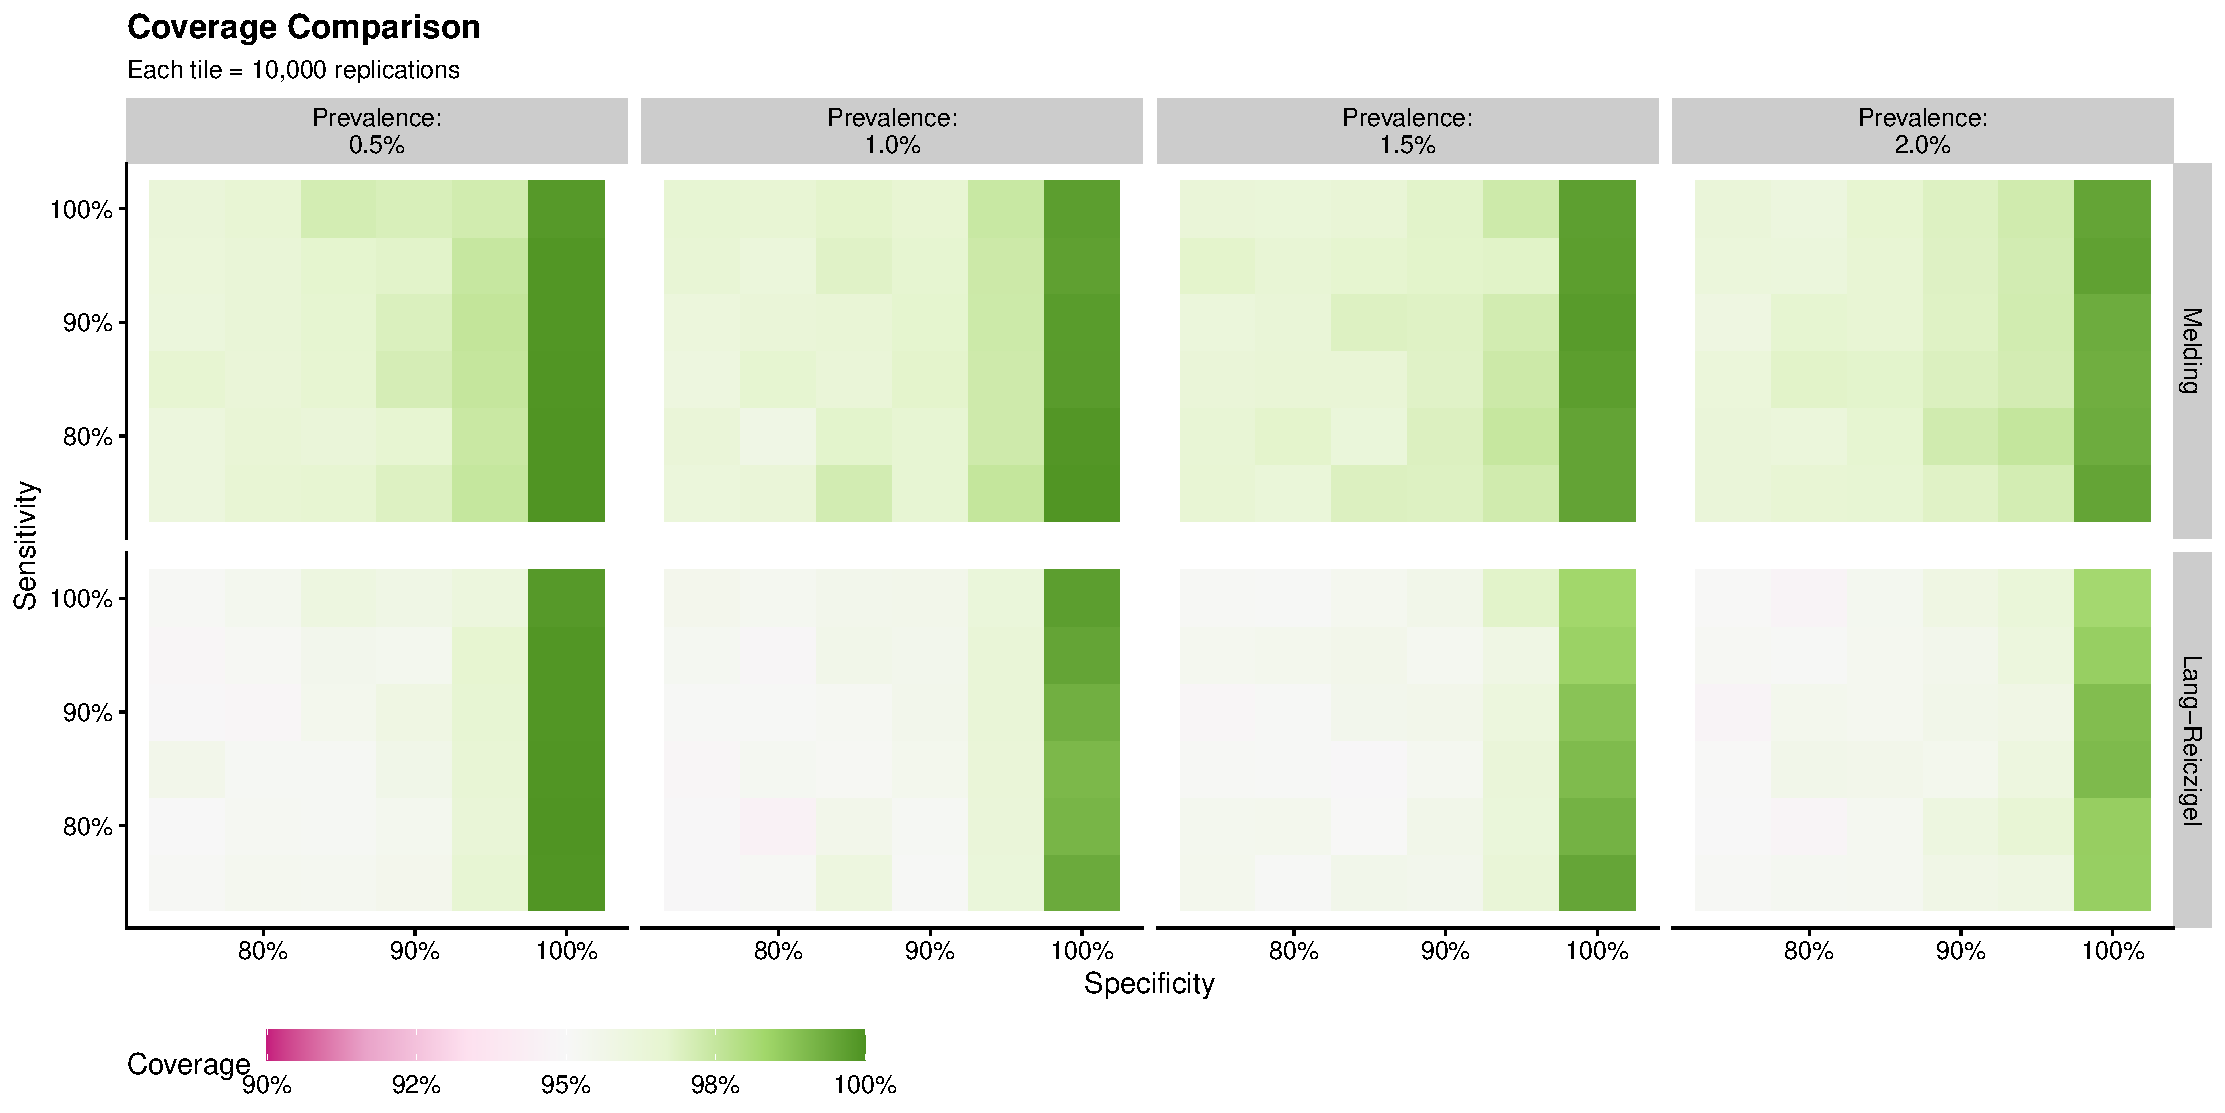
\includegraphics[width=0.8\textwidth]{figures/simple_coverage_comparison_plot.pdf}
    \caption{Coverage properties of 95\% confidence intervals for our new method (Melding) and the state of the art method (Lang-Reiczigel) in a variety of settings, each simulated 10,000 times.}
    \label{fig:coverage_comparison_plot}
\end{figure}

\begin{figure}
    \centering
    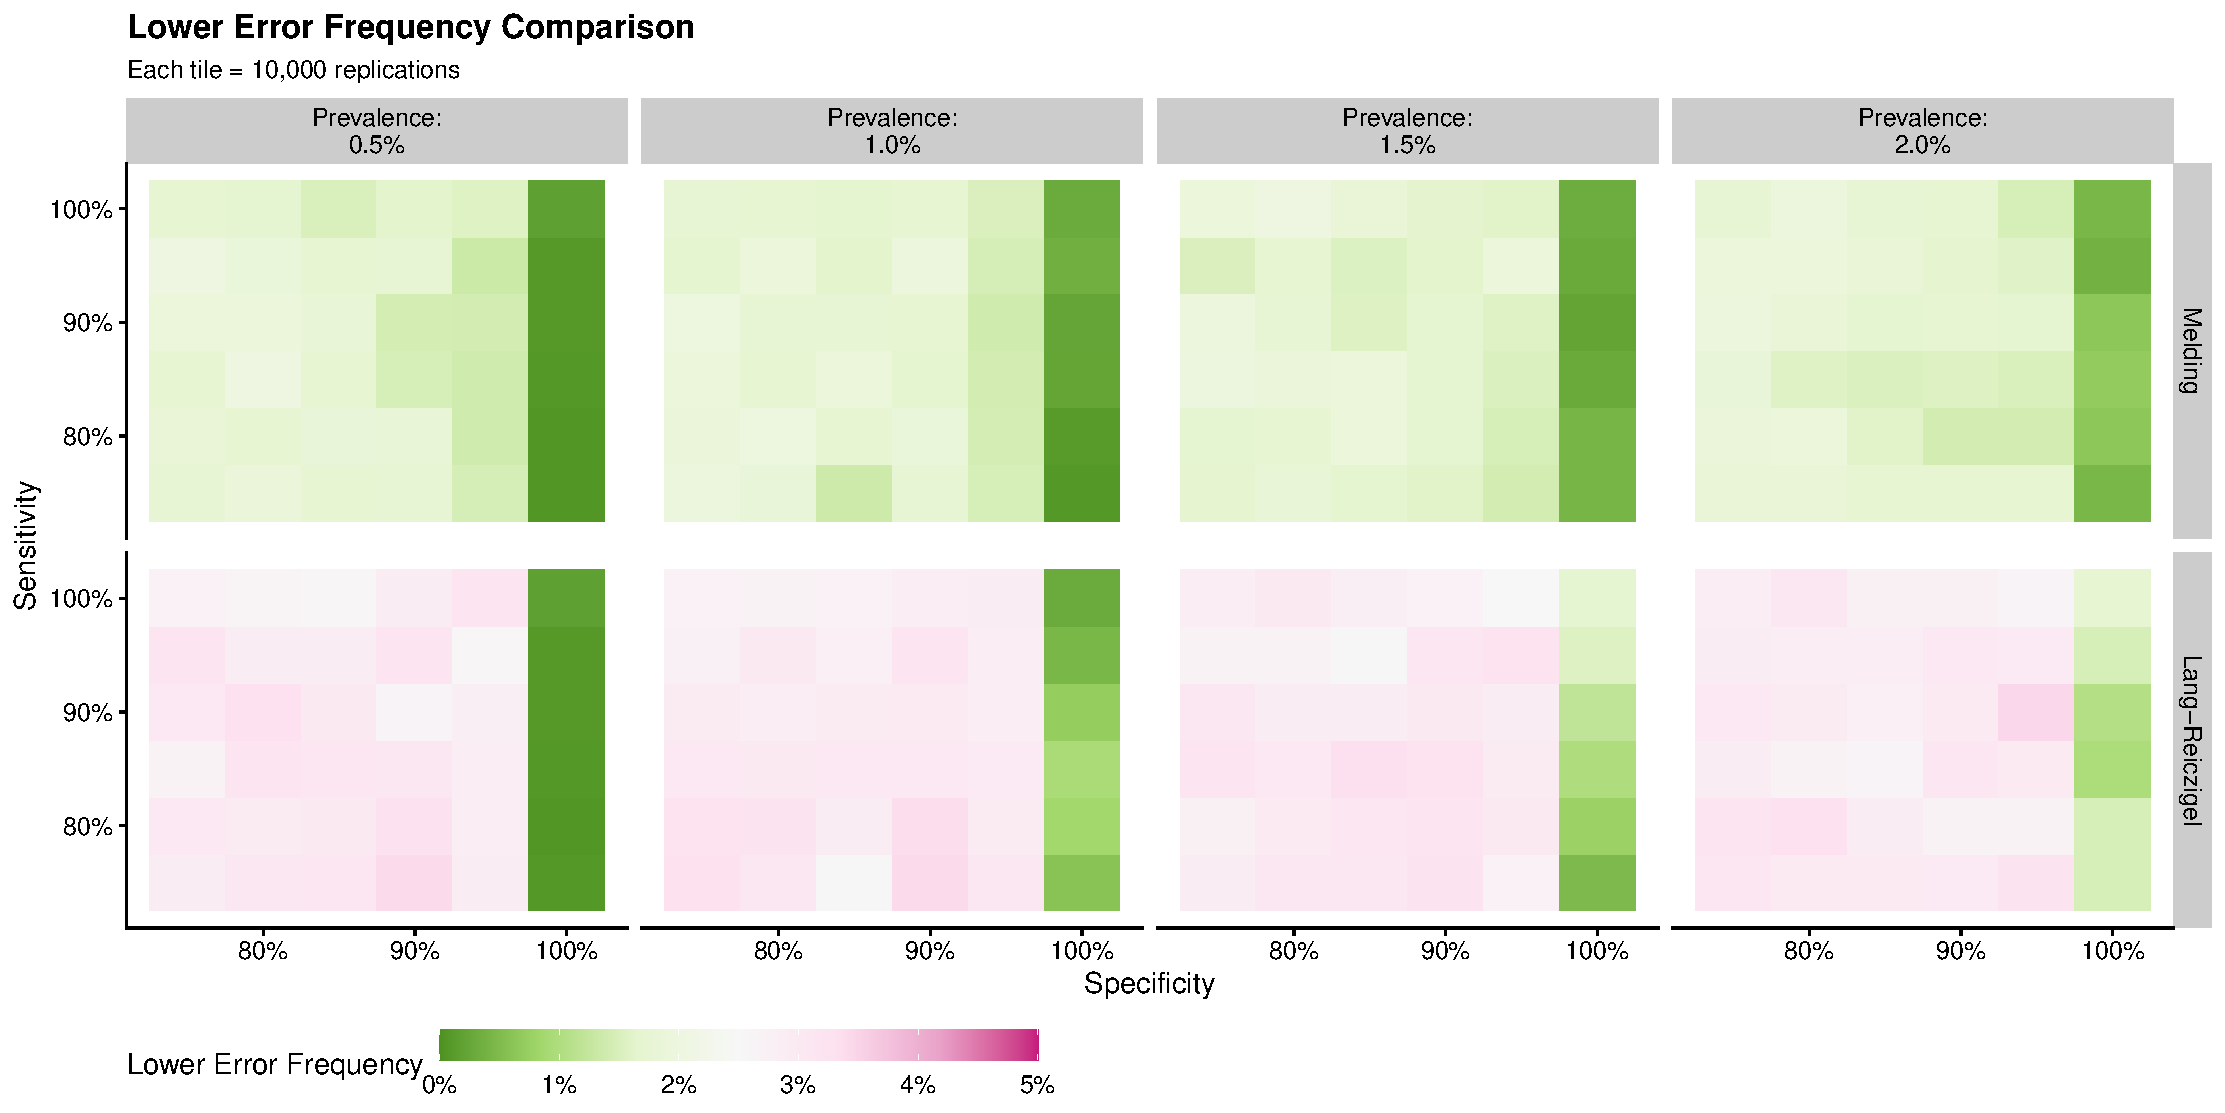
\includegraphics[width=0.8\textwidth]{figures/simple_lower_error_frequency_comparison_plot.pdf}
    \caption{Lower error properties of 95\% confidence intervals for our new method (Melding) and the state of the art method (Lang-Reiczigel) in a variety of settings, each simulated 10,000 times.}
    \label{fig:lower_error_frequency_comparison_plot}
\end{figure}

\begin{figure}
    \centering
    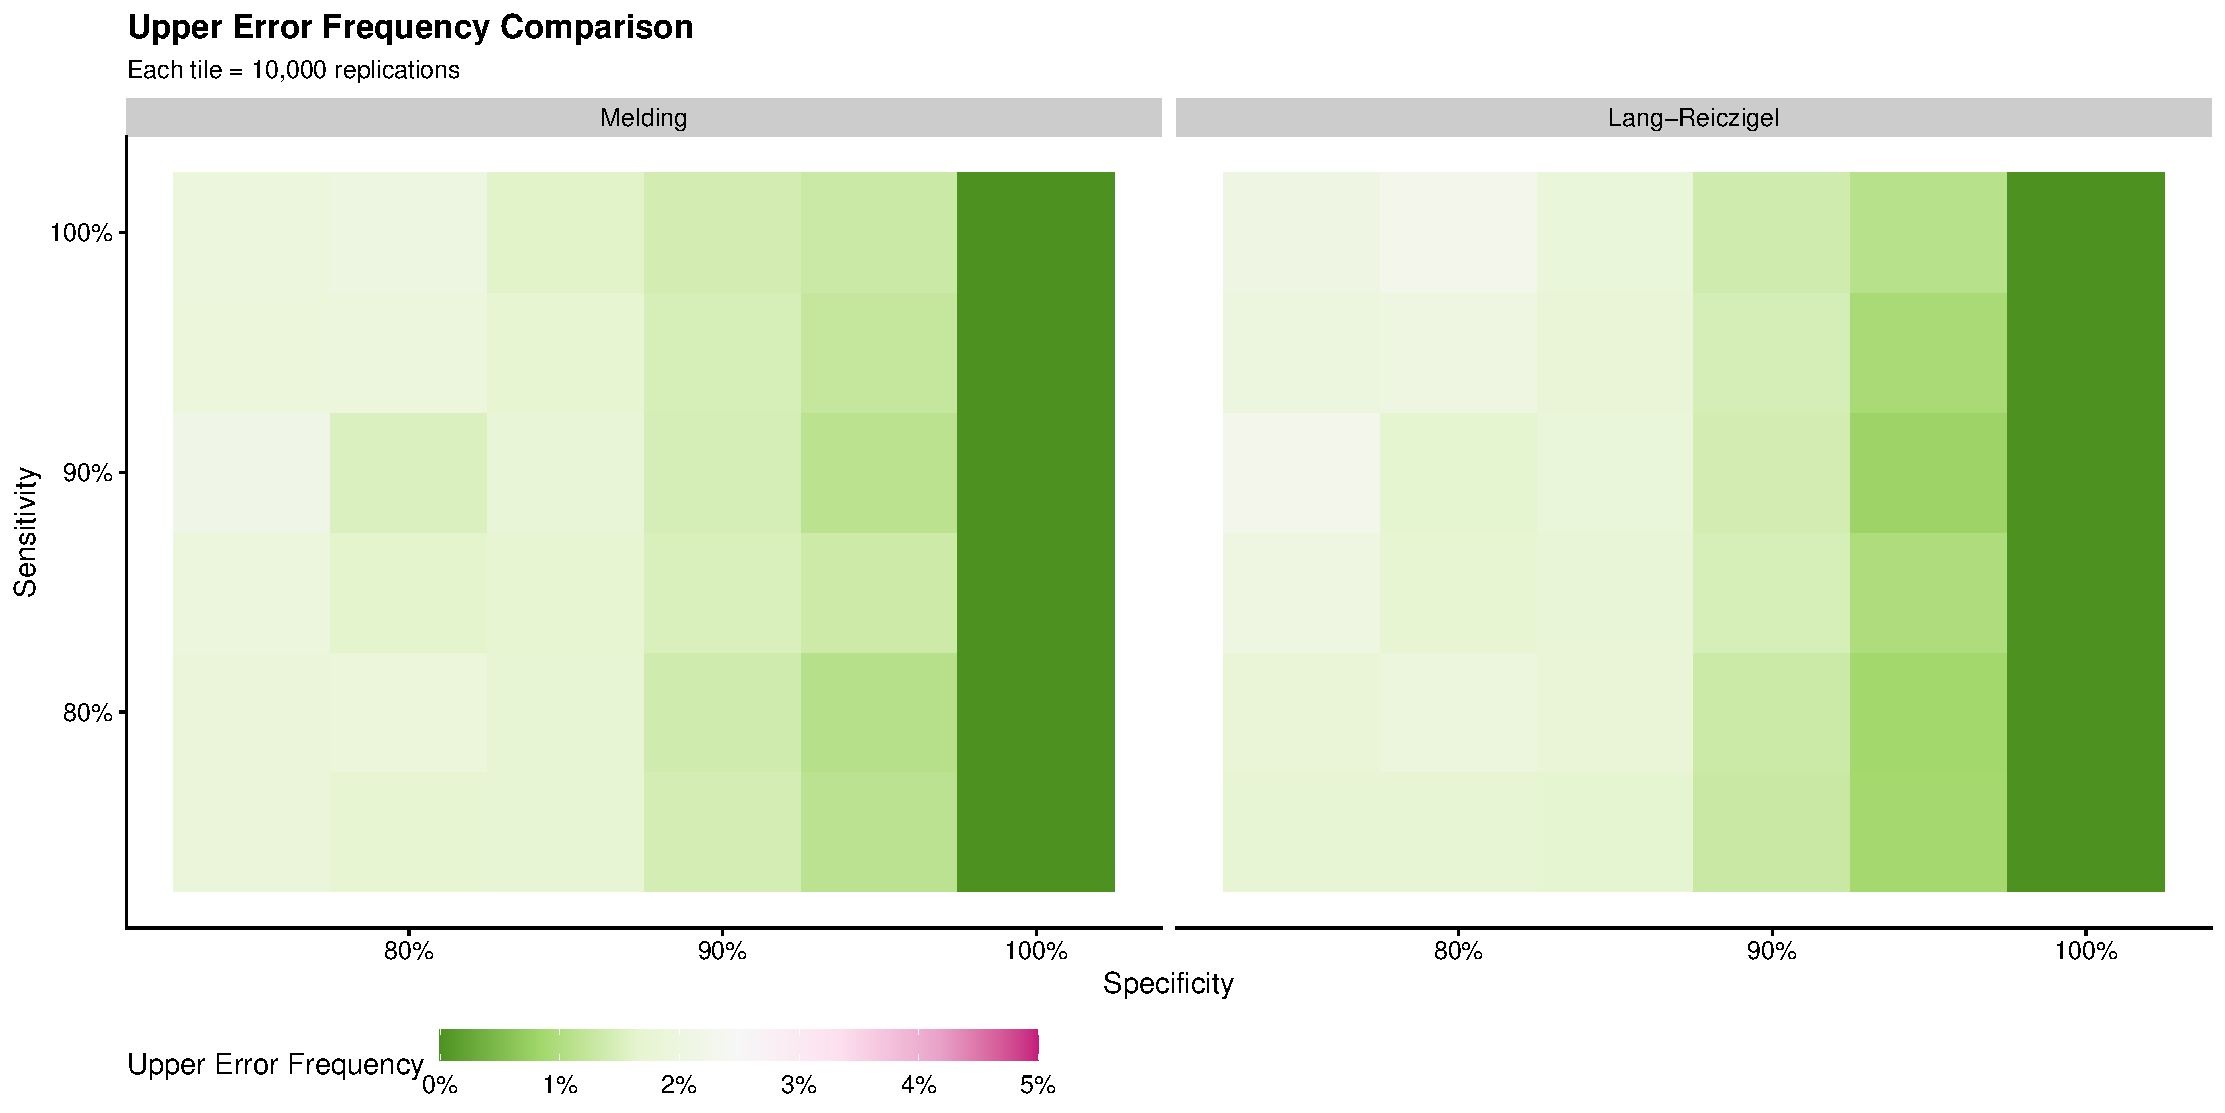
\includegraphics[width=0.8\textwidth]{figures/simple_upper_error_frequency_comparison_plot.pdf}
    \caption{Upper error properties of 95\% confidence intervals for our new method (Melding) and the state of the art method (Lang-Reiczigel) in a variety of settings, each simulated 10,000 times.}
    \label{fig:upper_error_frequency_comparison_plot}
\end{figure}

Figure~\ref{fig:coverage_comparison_plot} shows that, when specificity is less than perfect, both methods achieve approximately nominal coverage, with the melding method being somewhat more conservative.
When specificity is 100\%, both methods are conservative.
Figure~\ref{fig:upper_error_frequency_comparison_plot} shows that both methods make upper errors with roughly the same frequency.
Figure~\ref{fig:lower_error_frequency_comparison_plot} demonstrates that while the melding procedure leads bounds the lower error frequency below 2.5\%, the Lang-Reiczigel method is much more likely to lead to lower errors than it is to result in upper errors, which may be undesirable for applications that are particularly sensitive to making lower errors.


\subsection{Estimating Prevalence from a Weighted Sample with a Perfect Assay}

We compare the wsPoisson method to the more traditional Agresti-Coull and Korn-Graubard methods for survey proportions in a variety of settings.
Our simulations examine varying levels of disease prevalence (0.5\% or 5\%), types of groups surveyed (50 groups 200 subjects or 8000 groups of 1 subject), distributions of weights among the groups (coefficient of variation from approximately 0\% to nearly 6\%), the number of groups with non-zero prevalence, and the weights of the groups with non-zero prevalence.
For each scenario, 10,000 data sets are simulated and assessed.

\todo[inline]{Since our method is so conservative, I should look at the widths of the confidence intervals. Unfortunately, I have to re-reun simulations to do this.}

The coverage properties for these simulations are presented in Figures~\ref{fig:perfect_coverage_50_groups_0_005_prev}--\ref{fig:perfect_coverage_8000_groups_0_05_prev}.
Additional properties for these simulations are presented in Figures~\ref{fig:perfect_lower_error_frequency_50_groups_0_005_prev}--\ref{fig:perfect_upper_error_frequency_8000_groups_0_05_prev}.

From Figures~\ref{fig:perfect_coverage_50_groups_0_005_prev}--\ref{fig:perfect_coverage_8000_groups_0_05_prev}, we note that the two competitor methods generally exhibit lower coverage as the coefficient of variation among the weights increases.
In Figure~\ref{fig:perfect_coverage_50_groups_0_005_prev}, this coverage falls below 60\% when the prevalence very low and is concentrated among the highest weights, and the coefficient of variation among the weights exceeds 4.
Uniform distribution of prevalence among the weights, increased overall prevalence, and larger sample sizes among fewer groups all appear to lessen the severity of this problem.
In contrast, the wsPoisson method tends to become more conservative when the coefficient of variation among the weights increases.
In all cases, the wsPoisson method is more conservative than the competitor methods.
This is similar to the behavior observed in \cite{FayF:1997}, where, in simulations, the overall error rate decreased as the variance of the weights increased.

\begin{figure}
\centering
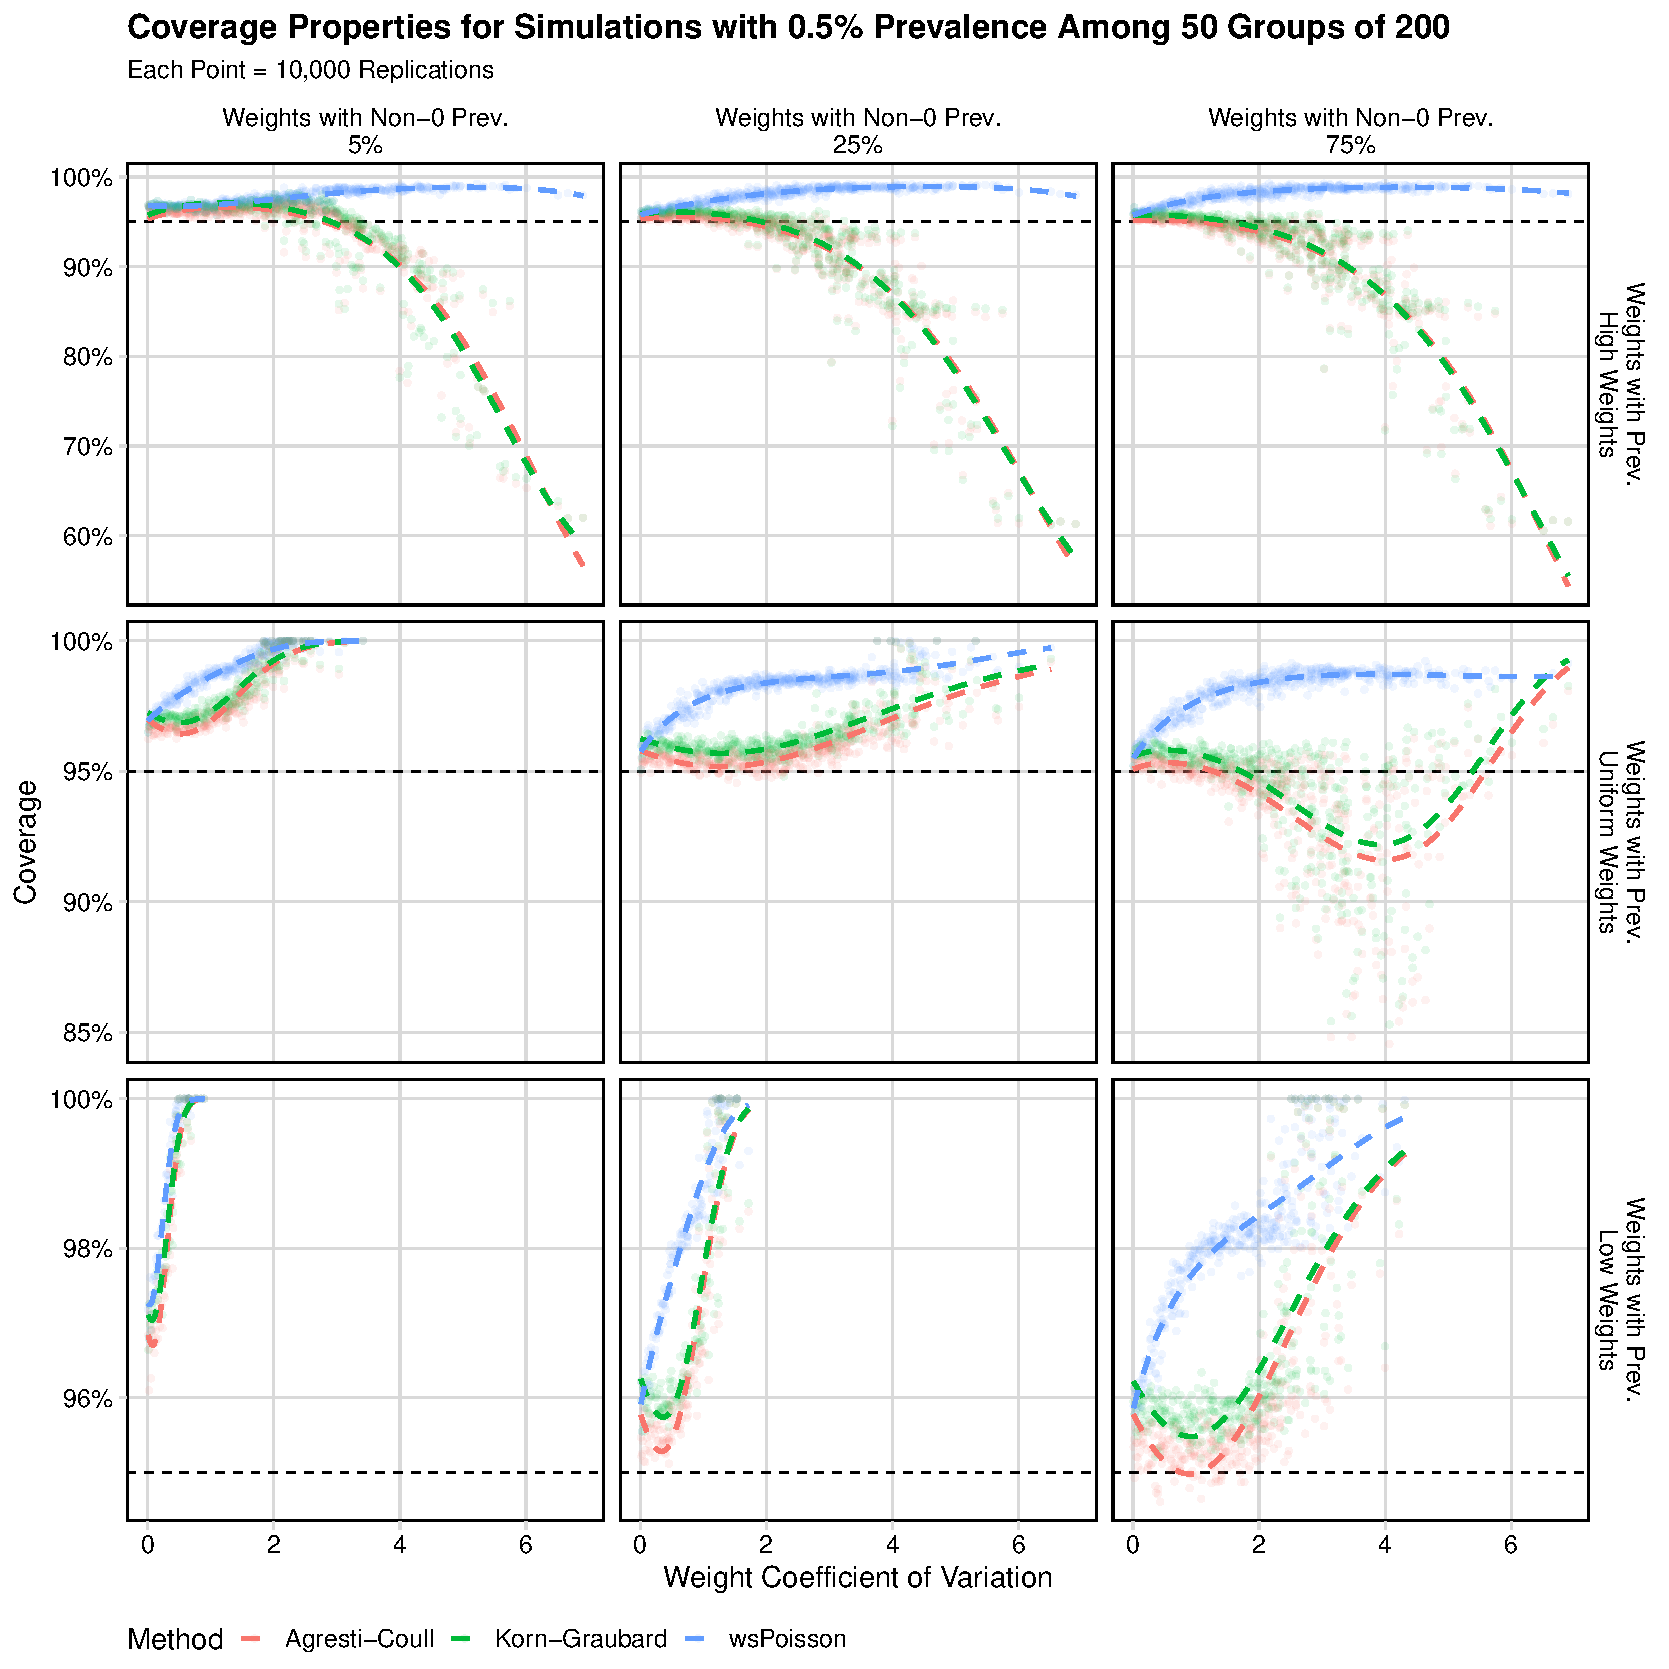
\includegraphics[width=0.8\textwidth]{figures/perfect_coverage_50_groups_0_005_prev.pdf}
\caption{Coverage properties for the wsPoisson model and two standard methods, Agresti-Coull and Clopper-Pearson.
Each point represents 10,000 simulations of datasets from a population with 0.5\% Prevalence where 50 groups of 200 people are sampled.
The horizontal dashed line indicates the nominal coverage, 95\%.
Colored dashed lines are estimates from a logistic regression model using cubic splines.}
\label{fig:perfect_coverage_50_groups_0_005_prev}
\end{figure}

\begin{figure}
\centering
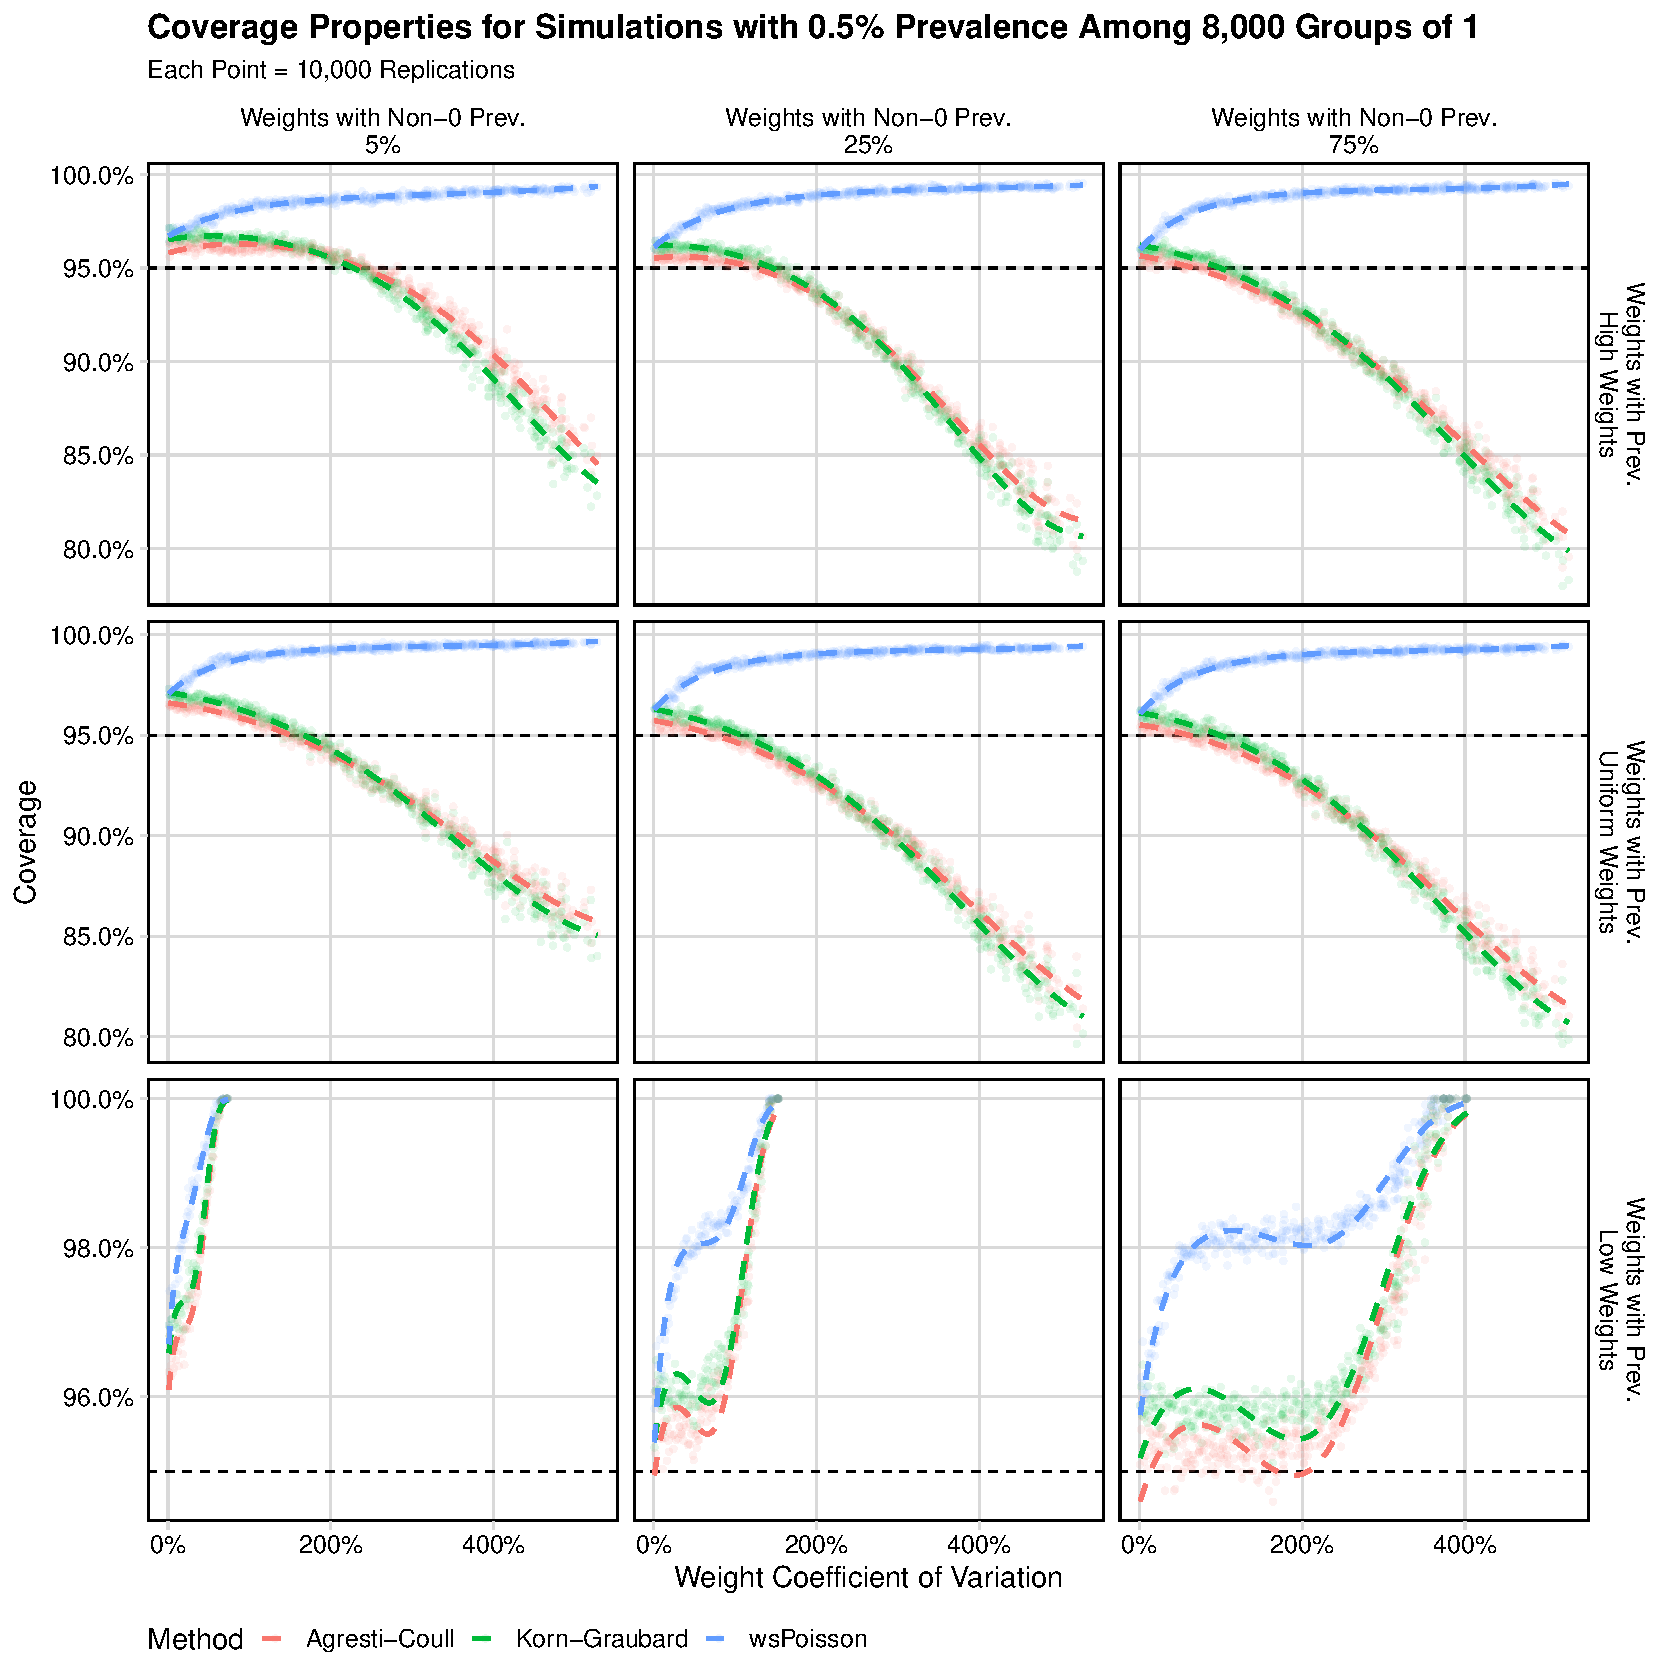
\includegraphics[width=0.8\textwidth]{figures/perfect_coverage_8000_groups_0_005_prev.pdf}
\caption{Coverage properties for the wsPoisson model and two standard methods, Agresti-Coull and Clopper-Pearson.
Each point represents 10,000 simulations of datasets from a population with 0.5\% Prevalence where 8000 individuals are sampled.
The horizontal dashed line indicates the nominal coverage, 95\%.
Colored dashed lines are estimates from a logistic regression model using cubic splines.}
\label{fig:perfect_coverage_8000_groups_0_005_prev}
\end{figure}

\begin{figure}
\centering
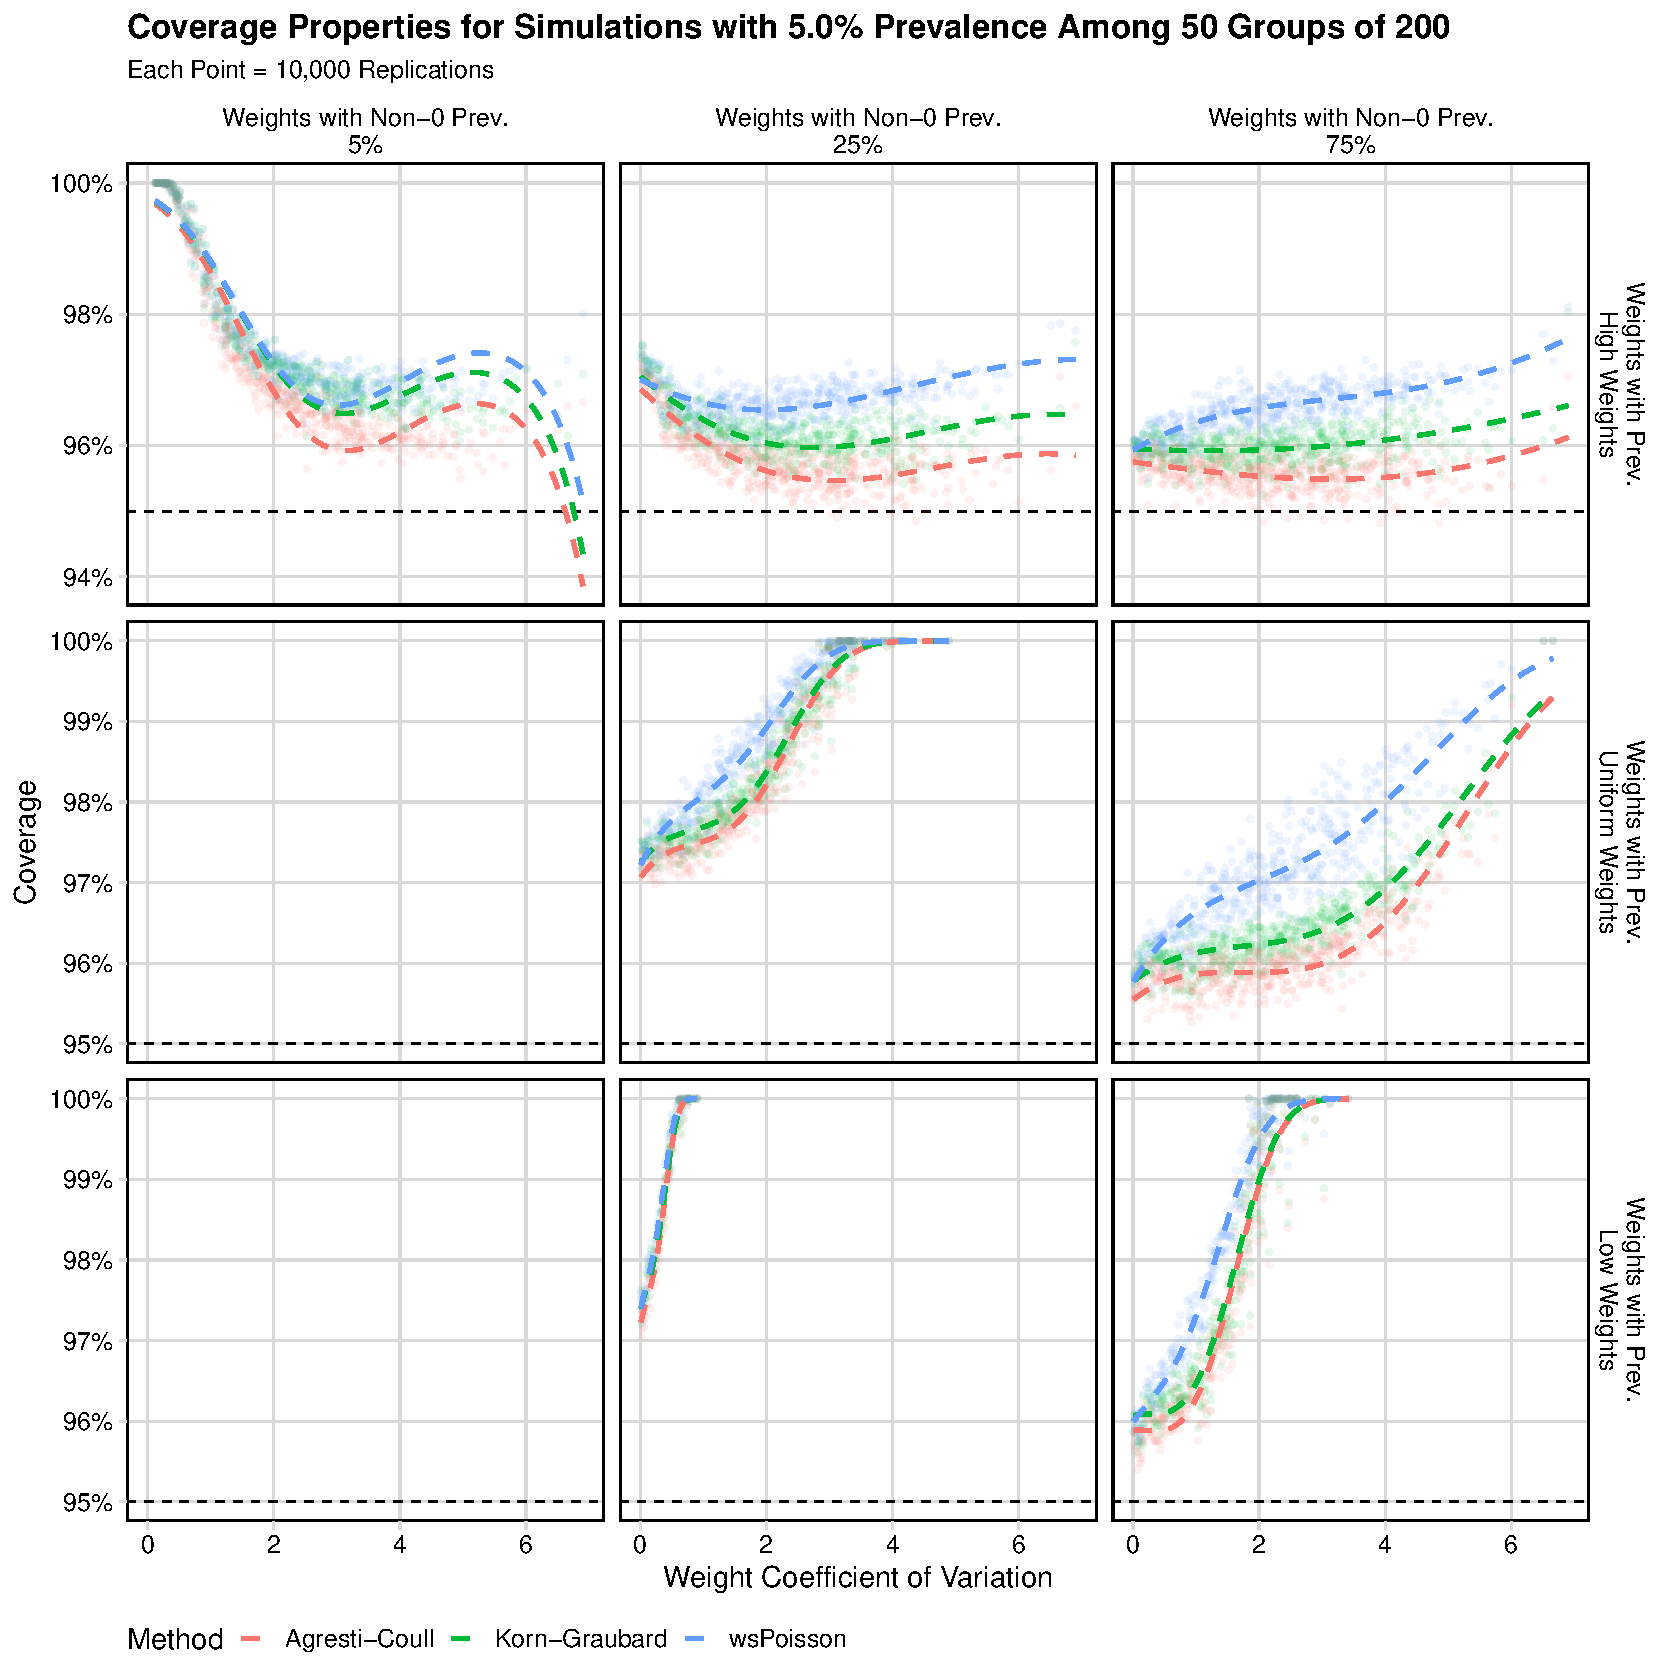
\includegraphics[width=0.8\textwidth]{figures/perfect_coverage_50_groups_0_05_prev.pdf}
\caption{Coverage properties for the wsPoisson model and two standard methods, Agresti-Coull and Clopper-Pearson.
Each point represents 10,000 simulations of datasets from a population with 5\% Prevalence where 50 groups of 200 people are sampled.
The horizontal dashed line indicates the nominal coverage, 95\%.
Colored dashed lines are estimates from a logistic regression model using cubic splines.}
\label{fig:perfect_coverage_50_groups_0_05_prev}
\end{figure}

\begin{figure}
\centering
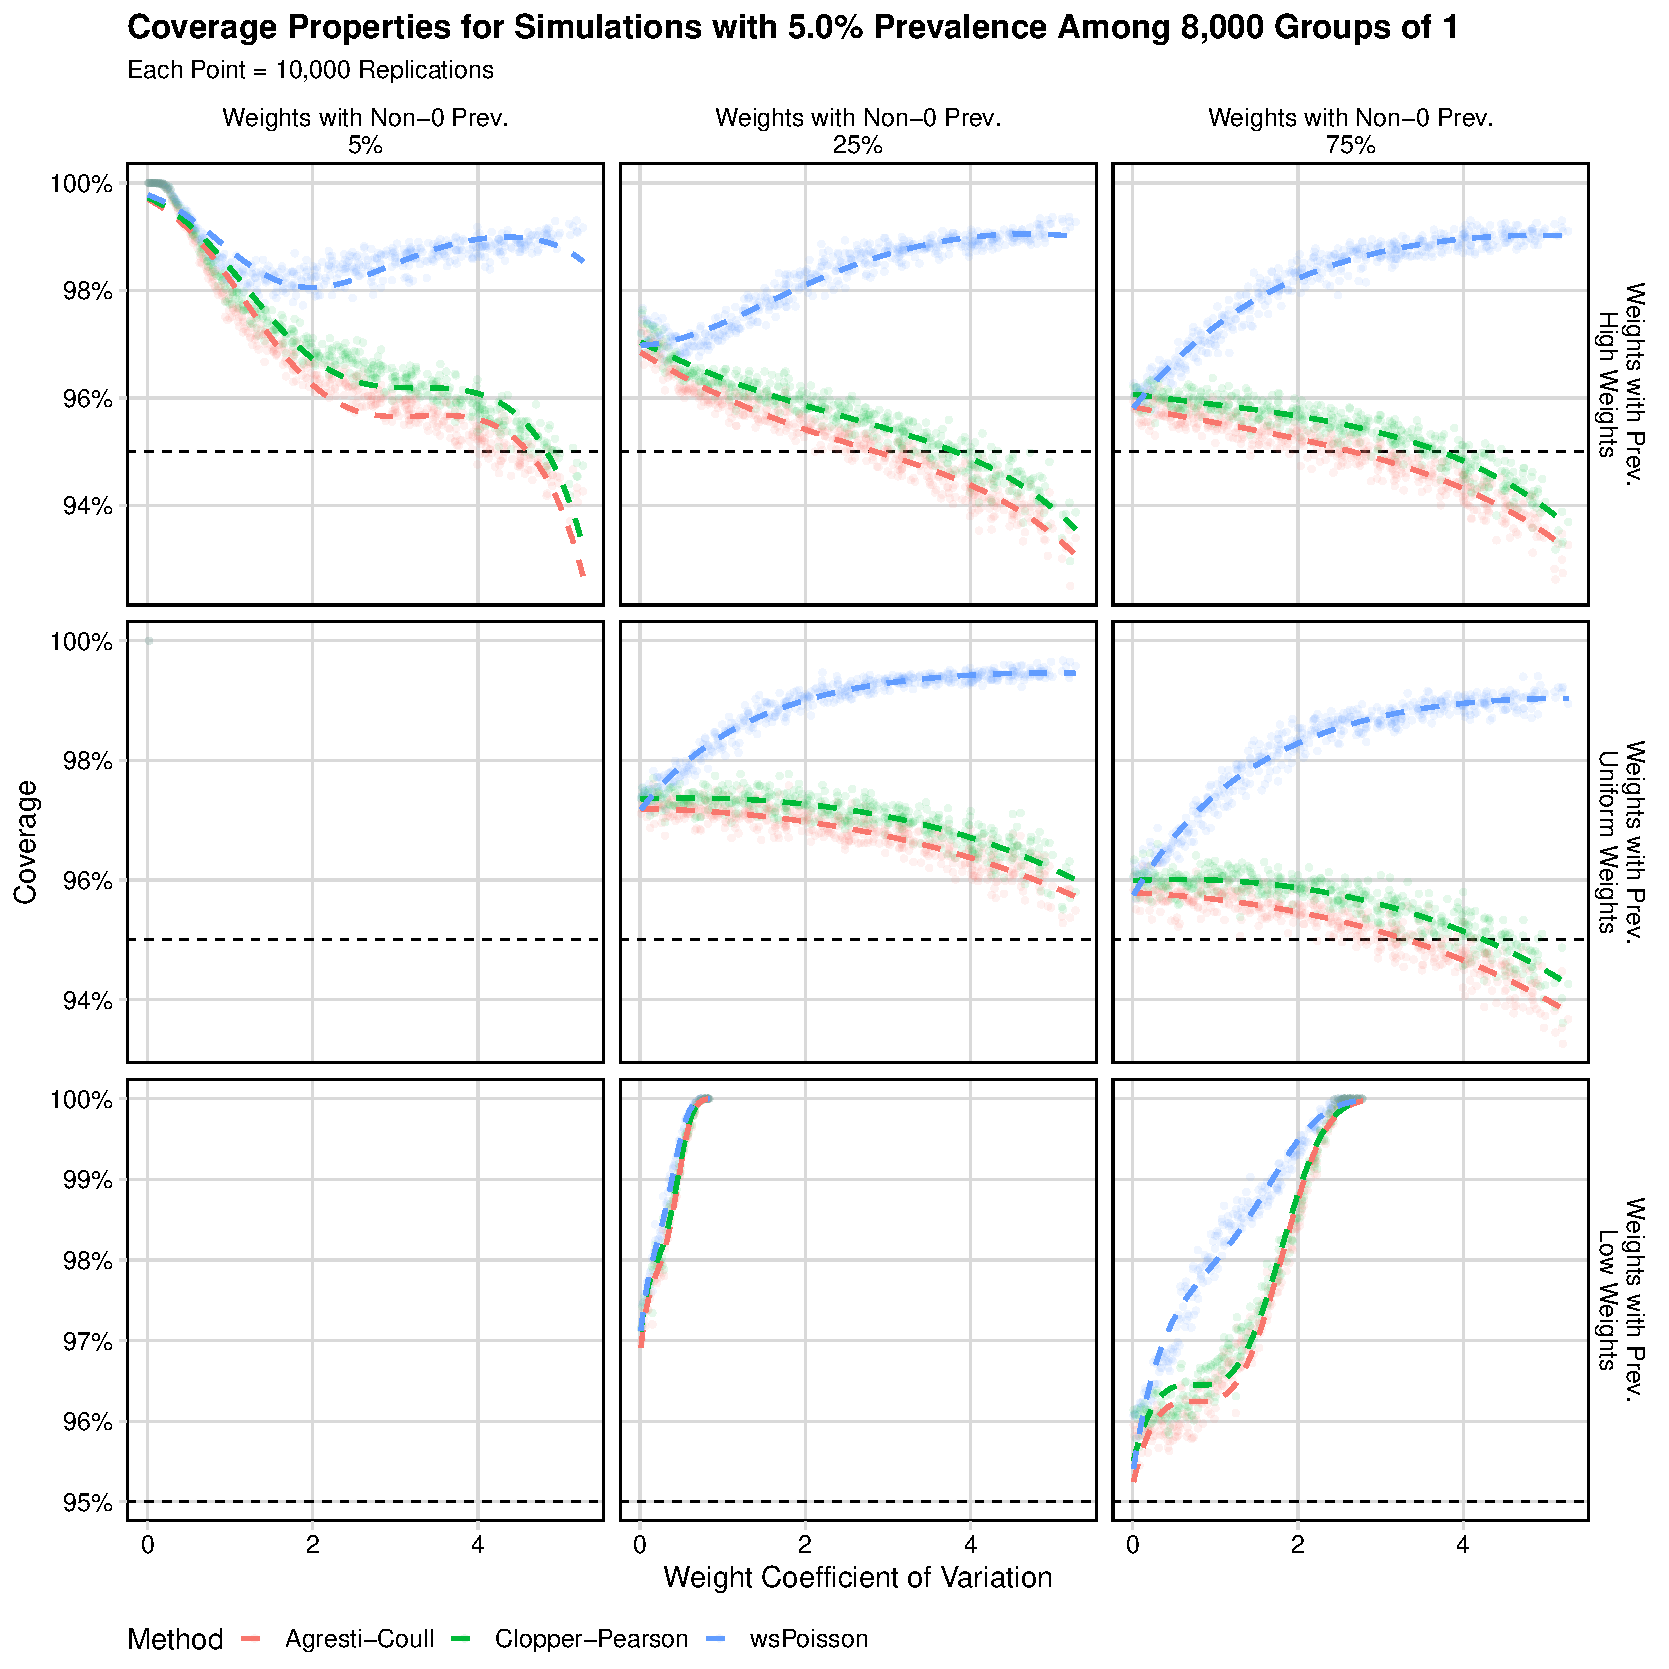
\includegraphics[width=0.8\textwidth]{figures/perfect_coverage_8000_groups_0_05_prev.pdf}
\caption{Coverage properties for the wsPoisson model and two standard methods, Agresti-Coull and Clopper-Pearson.
Each point represents 10,000 simulations of datasets from a population with 5\% Prevalence where 8000 individuals are sampled.
The horizontal dashed line indicates the nominal coverage, 95\%.
Colored dashed lines are estimates from a logistic regression model using cubic splines.}
\label{fig:perfect_coverage_8000_groups_0_05_prev}
\end{figure}


\subsection{Estimating Prevalence from a Weighted Sample with an Imperfect Assay}


We compare properties our melded confidence interval WprevSeSp Poisson, to anotother melded confidence interval method WprevSeSp Binomial, and one method, wspoissonTest, which does not account for the imperfect assay.
The methods are assessed in a several simulated scenarios with varying levels of disease prevalence (0.5\% or 5\%), types of groups surveyed (50 groups 200 subjects or 8000 groups of 1 subject), distributions of weights among the groups (coefficient of variation from approximately 0\% to nearly 6\%), the number of groups with non-zero prevalence, and the specificity of the assay (80\% - 100\%).
In each scenario, the assay has 95\% sensitivity.
Each scenario is simulated 10,000 times, with new prevalence, sensitivity, and specificity surveys generated and 95\% confidence intervals are created.
Simulated sensitivity is assessed based on 60 tests, while specificity is based on 300 tests.

\todo[inline]{Since our method is so conservative, I should look at the widths of the confidence intervals. Unfortunately, I have to re-reun simulations to do this.}

The coverage properties for these simulations are presented in Figures~\ref{fig:imperfect_coverage_50_groups_0_005_prev}--\ref{fig:imperfect_coverage_8000_groups_0_05_prev}.
Additional properties for these simulations are presented in Figures~\ref{fig:imperfect_lower_error_frequency_50_groups_0_05_prev}--\ref{fig:imperfect_upper_error_frequency_8000_groups_0_05_prev}.

\begin{figure}
\centering
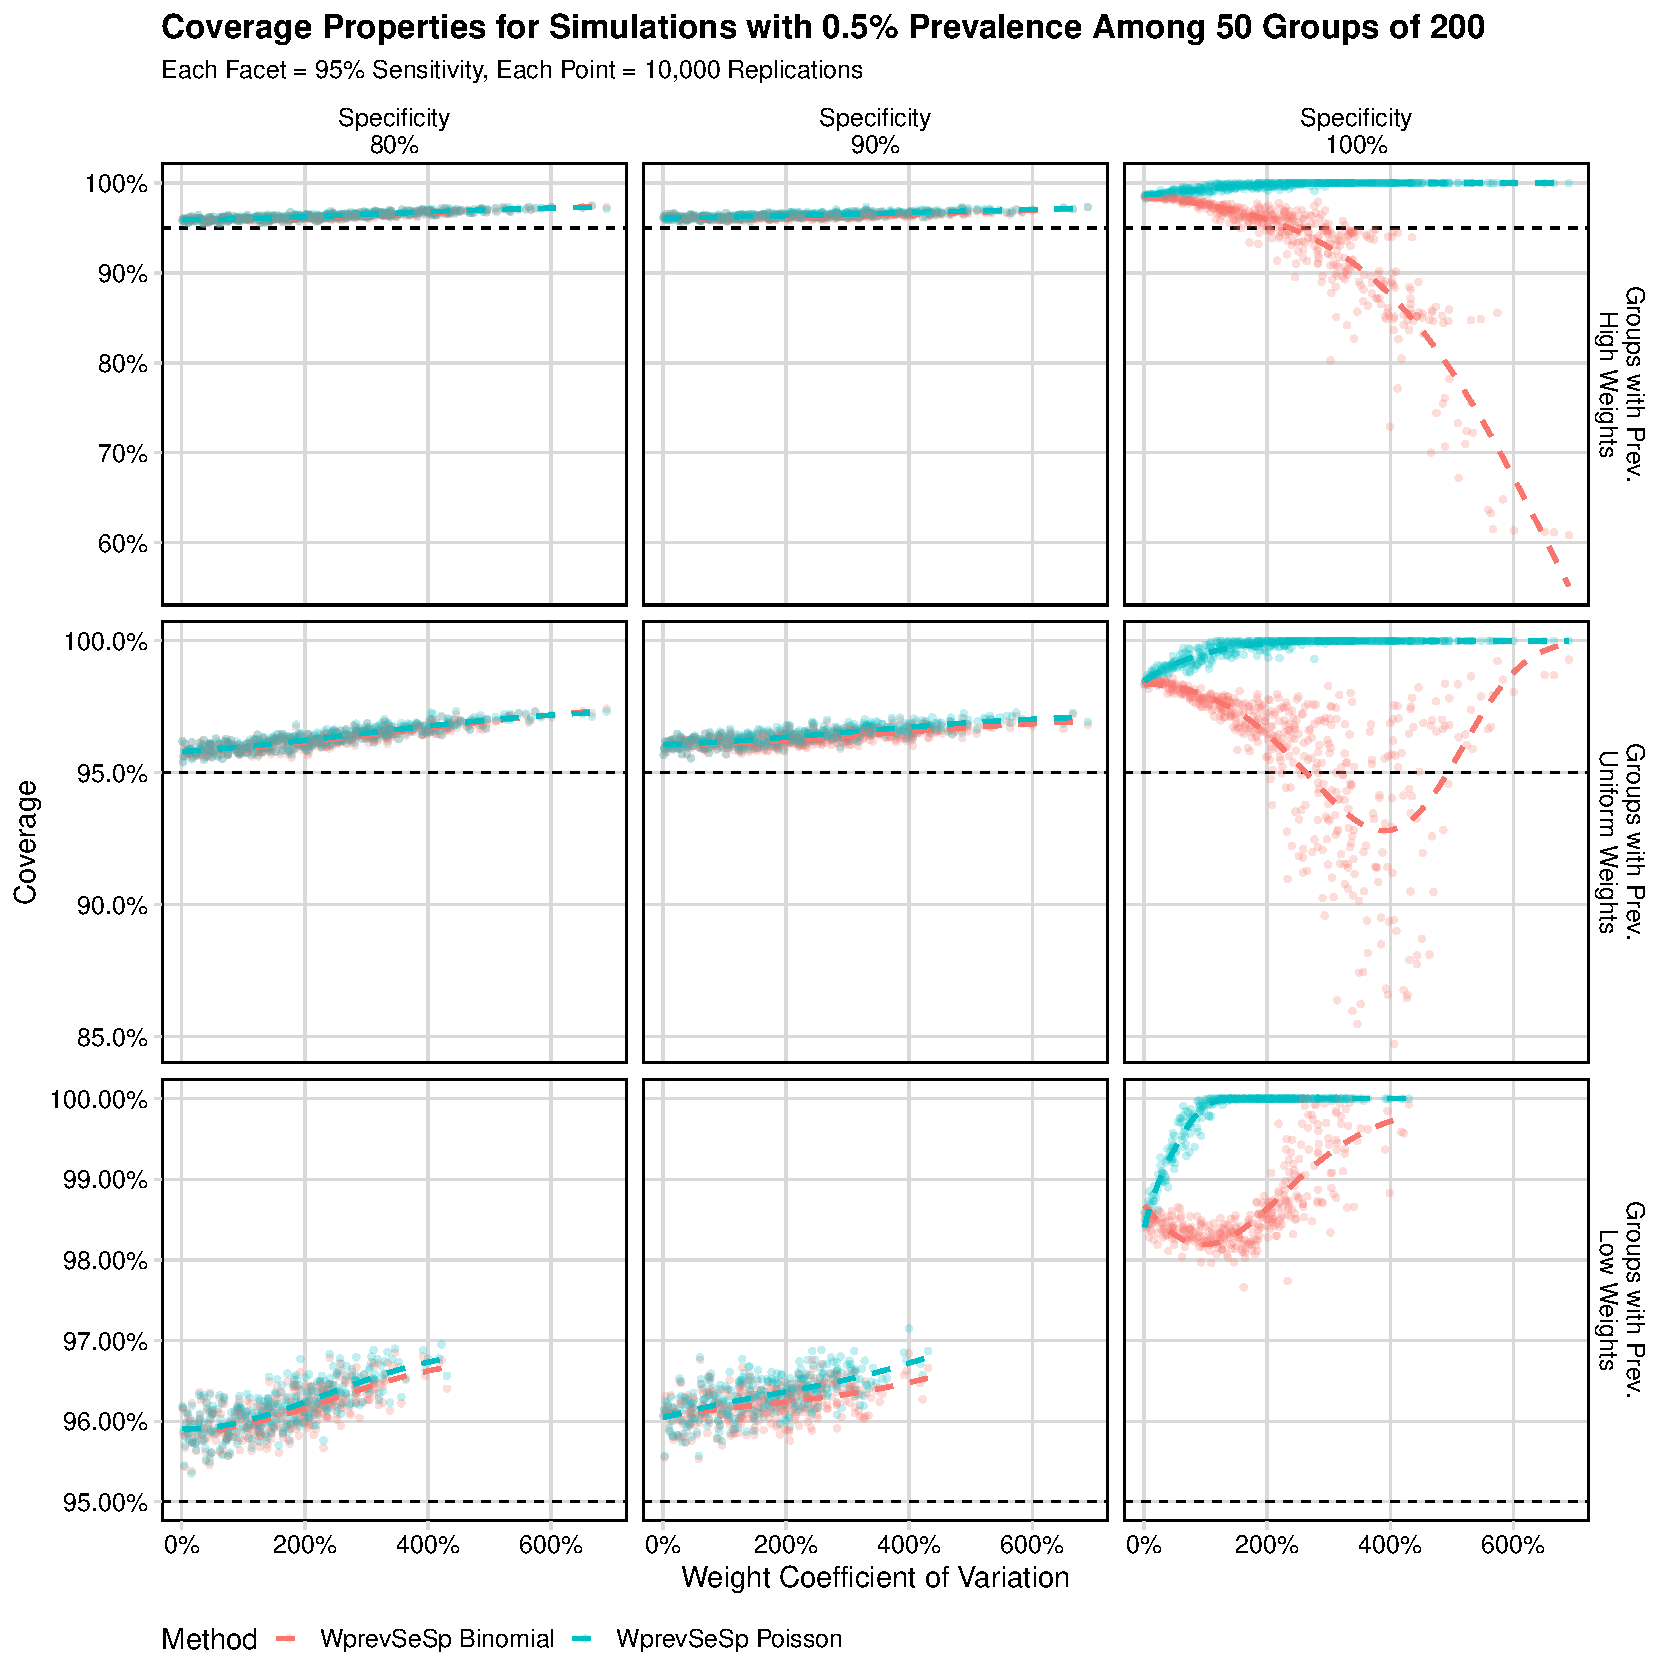
\includegraphics[width=0.8\textwidth]{figures/imperfect_coverage_50_groups_0_005_prev.pdf}
\caption{Coverage properties for the two melded confidence interval procedures, WprevSeSp Binomial and WprevSeSp Poisson, and one method, wspoissonTest, which does not account for the imperfect assay.
Each point represents 10,000 simulations of datasets from a population with 0.5\% Prevalence where 50 groups of 200 people are sampled.
Each datasets also includes simulated results of tests to evaluate the sensitivity and specificity of the assay performed on 60 and 300 individuals, respectively.
The horizontal dashed line indicates the nominal coverage, 95\%.
Colored dashed lines are estimates from a logistic regression model using cubic splines.}
\label{fig:imperfect_coverage_50_groups_0_005_prev}
\end{figure}

\begin{figure}
\centering
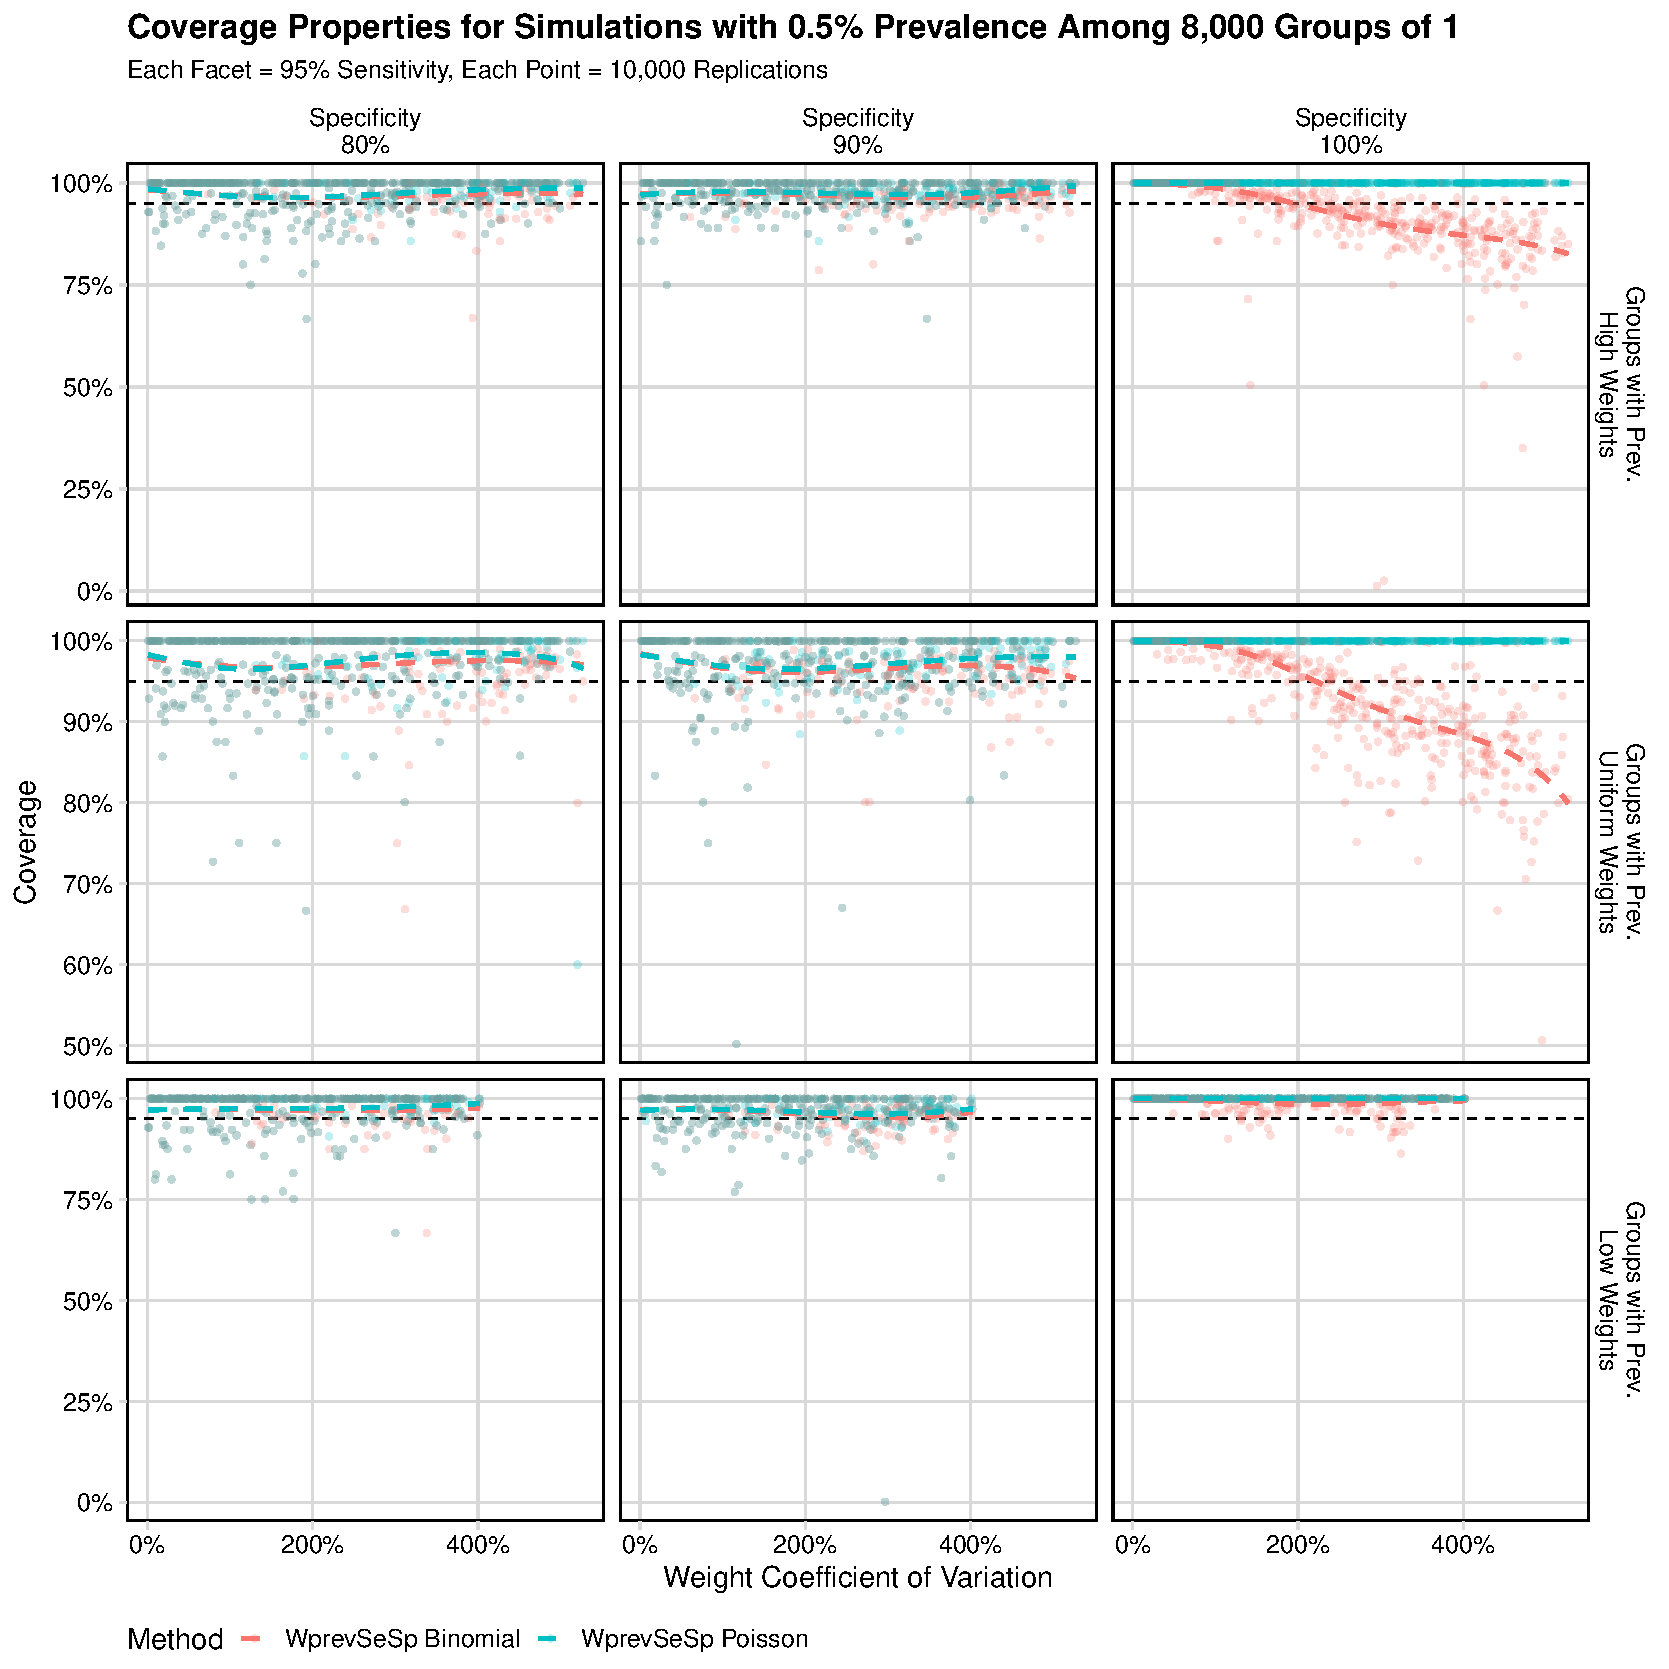
\includegraphics[width=0.8\textwidth]{figures/imperfect_coverage_8000_groups_0_005_prev.pdf}
\caption{Coverage properties for the two melded confidence interval procedures, WprevSeSp Binomial and WprevSeSp Poisson, and one method, wspoissonTest, which does not account for the imperfect assay.
Each point represents 10,000 simulations of datasets from a population with 0.5\% Prevalence where 8000 individuals are sampled.
Each datasets also includes simulated results of tests to evaluate the sensitivity and specificity of the assay performed on 60 and 300 individuals, respectively.
The horizontal dashed line indicates the nominal coverage, 95\%.
Colored dashed lines are estimates from a logistic regression model using cubic splines.}
\label{fig:imperfect_coverage_8000_groups_0_005_prev}
\end{figure}

\begin{figure}
\centering
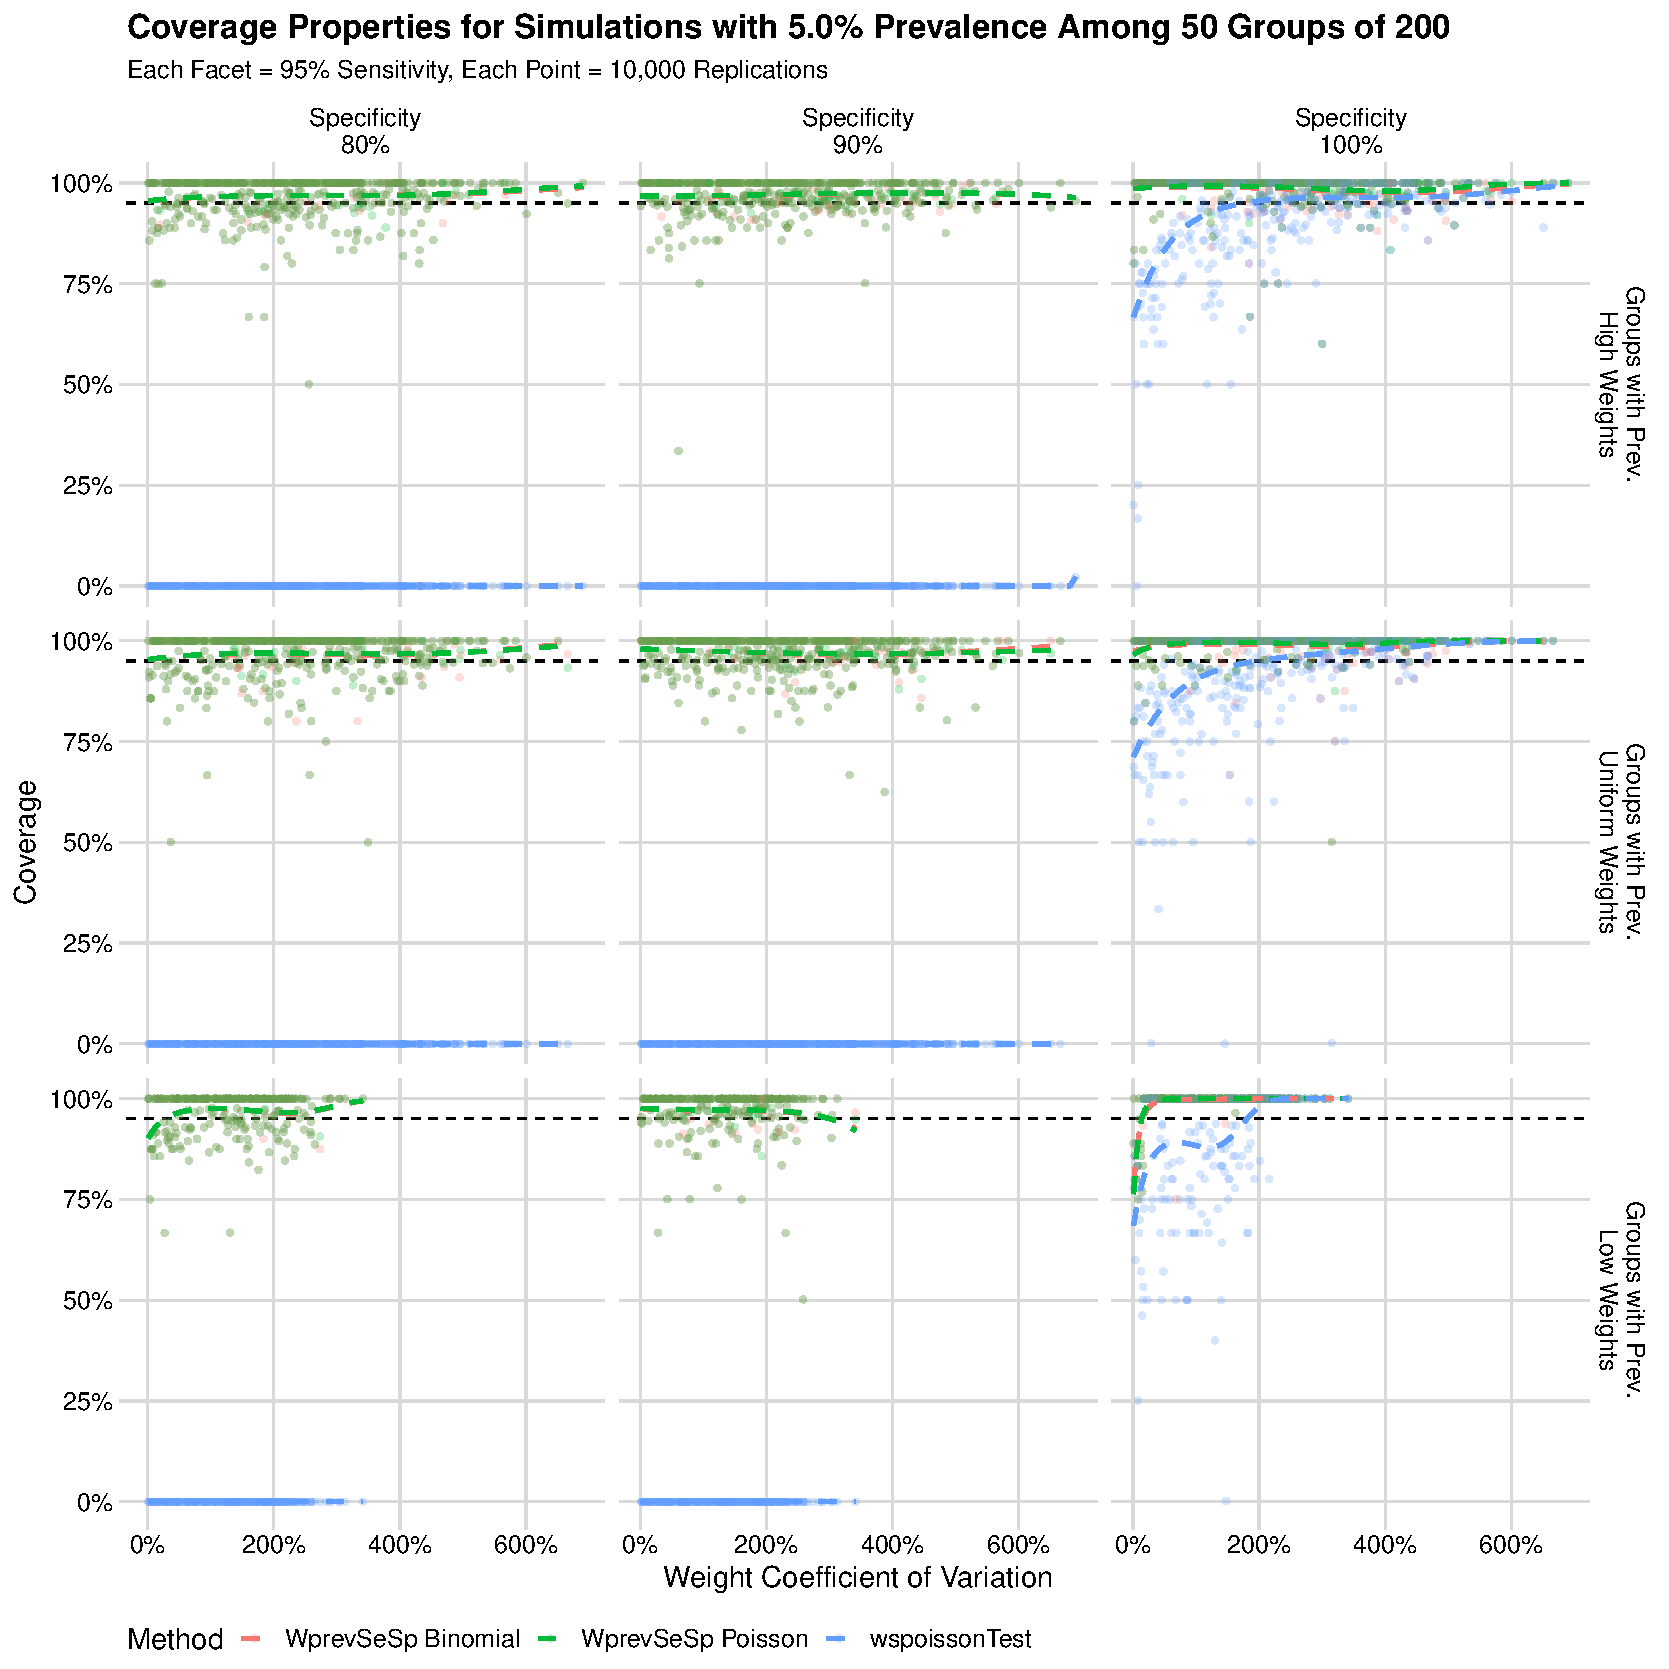
\includegraphics[width=0.8\textwidth]{figures/imperfect_coverage_50_groups_0_05_prev.pdf}
\caption{Coverage properties for the two melded confidence interval procedures, WprevSeSp Binomial and WprevSeSp Poisson, and one method, wspoissonTest, which does not account for the imperfect assay.
Each point represents 10,000 simulations of datasets from a population with 5\% Prevalence where 50 groups of 200 people are sampled.
Each datasets also includes simulated results of tests to evaluate the sensitivity and specificity of the assay performed on 60 and 300 individuals, respectively.
The horizontal dashed line indicates the nominal coverage, 95\%.
Colored dashed lines are estimates from a logistic regression model using cubic splines.}
\label{fig:imperfect_coverage_50_groups_0_05_prev}
\end{figure}

\begin{figure}
\centering
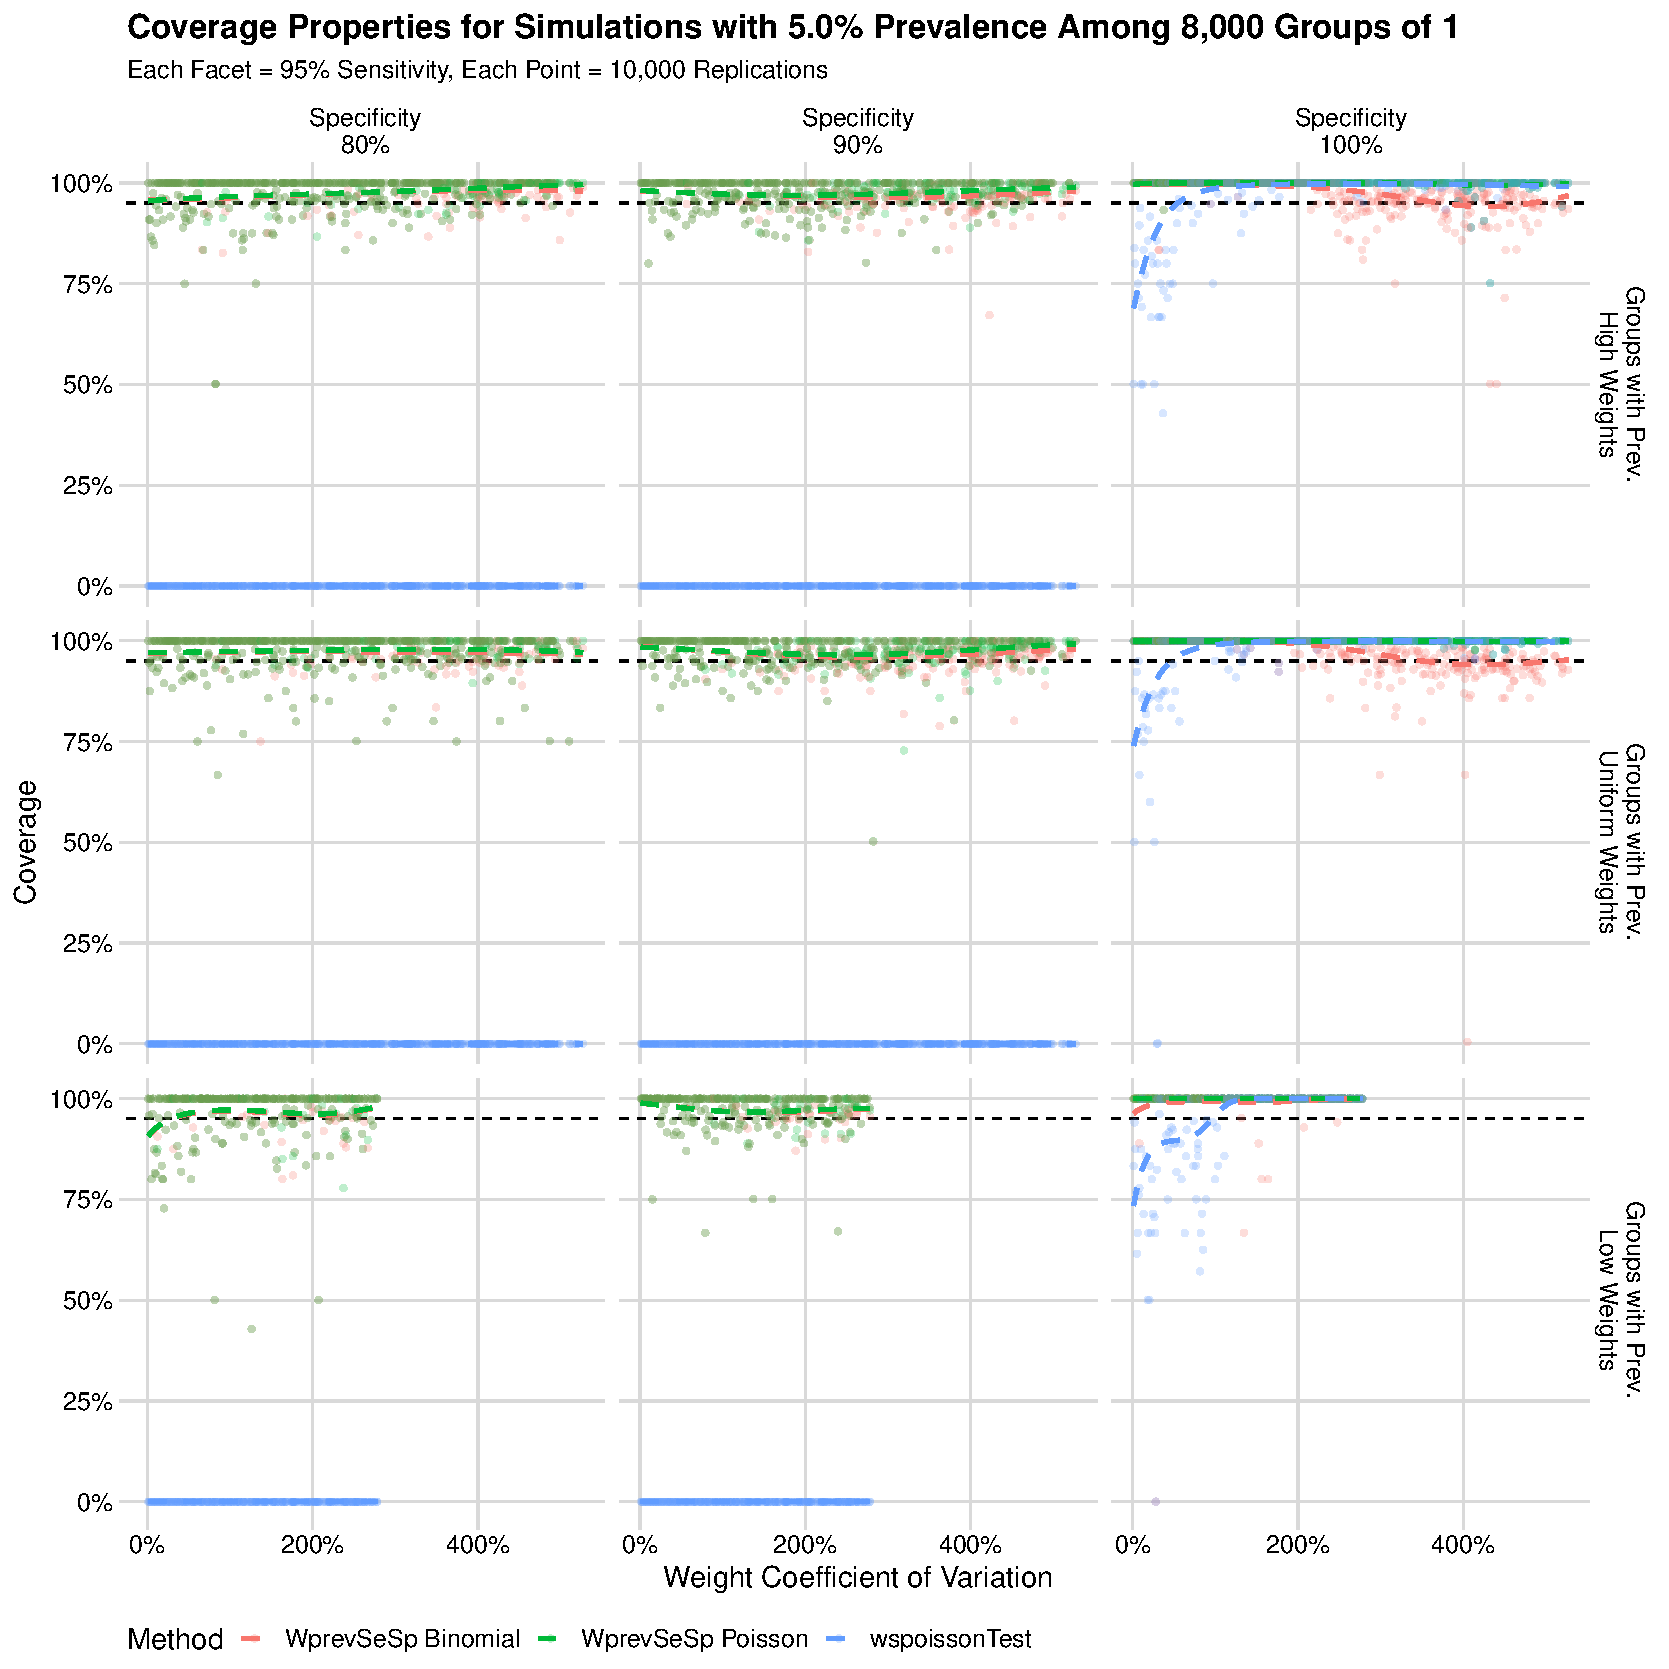
\includegraphics[width=0.8\textwidth]{figures/imperfect_coverage_8000_groups_0_05_prev.pdf}
\caption{Coverage properties for the two melded confidence interval procedures, WprevSeSp Binomial and WprevSeSp Poisson, and one method, wspoissonTest, which does not account for the imperfect assay.
Each point represents 10,000 simulations of datasets from a population with 5\% Prevalence where 8000 individuals are sampled.
Each datasets also includes simulated results of tests to evaluate the sensitivity and specificity of the assay performed on 60 and 300 individuals, respectively.
The horizontal dashed line indicates the nominal coverage, 95\%.
Colored dashed lines are estimates from a logistic regression model using cubic splines.}
\label{fig:imperfect_coverage_8000_groups_0_05_prev}
\end{figure}

Based on Figures~\ref{fig:imperfect_lower_error_frequency_50_groups_0_05_prev}--\ref{fig:imperfect_upper_error_frequency_8000_groups_0_05_prev}, we note that, in most settings, the naive wspoissonTest procedure results in extremely poor coverage, around 0\%, while the two melding procedures result in conservative confidence intervals, often nearing 100\% coverage.
With perfect specificity, the issue of poor coverage for the wspoissonTest procedure is less prominent, but the WprevSeSp Binomial method fails to maintain nominal coverage when the coefficient of variation among the weights is high.
Only our proposed WprevSeSp Poisson method maintains or exceed the desired coverage in all scenarios.

We also apply these two methods to a real data set from \cite{Kali:2021}.
This data set was collected to estimate seroprevalence of SARS-CoV-2 in the United States between May and July 2020.
This test used in this data is estimated to have perfect sensitivity, based on 56 tests on individuals with confirmed SARS-CoV-2 and perfect specificity based on 300 tests on individuals confirmed to not have SARS-CoV-2.
First we apply the methods to the full data set (\( n =  8058, \text{weight coefficient of variation} = 252\%\)).
The Korn and Graubard type melded confidence interval (WprevSeSp Binomial) produced the 95\% confidence interval for population prevalence (2.53\%, 6.68\%), while the wsPoisson type melded confidence interval (WprevSeSp Poisson) produce the 95\% confidence interval (2.56\%, 7.54\%).
We also apply the wspoissonTest method from Section~\ref{sec:weight-perfect}, which does not account for imperfections in the assay, resulting in a 95\% confidence interval of (3.04\%, 7.39\%).
While all three intervals overlap to a large degree, the wsPoisson type melded confidence interval is the widest.
Our simulations show that the three procdures have similar coverage when specificity and weight coefficient of variation are both high, so this is unsurprising.


We also apply the methods to the subset of only Hispanic participants (\( n = 1281, \text{weight coefficient of variation} = 306\% \)).
The Korn and Graubard type confidence distributions (WprevSeSp Binomial) produce the 95\% confidence interval for population prevalence (2.35\%, 11.75\%), while the wsPoisson type confidence distributions (WprevSeSp Poisson) produce the 95\% confidence interval (2.40\%, 20.02\%).
The wspoissonTest method produces a 95\% confidence interval of (2.80\%, 19.63\%).
In this case, the two melded confidence intervals are much wider than the naive interval, as expected.
This is somewhat unexpected, but may be because prevalence is concentrated among respondents with lower weights, or be related to the smaller sample size used to measure prevalence, which is not reflected in our simulations.

\pagebreak

% Misc quotes from Mike to incorporate:

% \begin{itemize}
%     \item The last time we met, you mentioned that it would be nice to report the weights in terms of coefficient of variation. I went back to the data from the COVID seroprevalence paper in undiagnosed adults, and I calculated a coefficient of variation  of 2.52 = 252\% for all 8058 individuals, and looking at subsets, I found that the Hispanics had a CV=306\%.  
%     \item For some weighting for surveys to adjust for selection bias, the coefficient of variation may be large.  For example, the coefficient of variation of the weights (CVW) for the main estimate of seroprevalence in Kalish, et al (2021) had CVW=252\%, and it could be even larger for subsets of the population (e.g., Hispanics had CVW=306\%). 
% \end{itemize}



\section{Discussion}

We presented several methods for creating confidence to assess disease prevalence in variety of settings, including simple random samples with imperfect tests, weighted sampling with perfect tests, and weighted sampling with imperfect tests.
As a general theme, these confidence intervals tend to demonstrate higher coverage than competitor methods.
In the case of the simple random sample with an imperfect test, we are able to bound the lower error rate for a 95\% confidence interval at 2.5\%, while the state-of-the-art method maintains 95\% coverage by allowing a higher lower error rate.
Our methods' conservative properties are especially advantageous in settings where the competitor methods exhibit much lower than nominal coverage.
For example, there is high variance among the sample weights and prevalence is concentrated among the highest-weighted samples competitor coverage of 95\% confidence intervals can fall to 60\% for competitor methods, while our method exhibits > 95\% coverage.
Thus, we suggest that our melding methods be employed when working with survey settings which involve high variance among the weights or lower errors are particularly undesirable.

% \acks
% \begin{acks}
\section{Acknowledgements}
For sharing the data from the Kalish, et al study, we thank Matthew Memoli and the LID Clinical Studies Unit of the National Institute of Allergy and Infectious Diseases, NIH,  Kaitlyn Sadtler from the National Institute of Biomedical Imaging and Bioengineering, NIH,   Matthew Hall from the National Center for Advancing Translational Sciences, NIH, and Dominic Esposito from the Fredrick National Laboratory for Cancer Research, NCI, NIH.
% \end{acks}

\section{Bibliography}
\nocite{*}% Show all bib entries - both cited and uncited; comment this line to view only cited bib entries;
\bibliography{refs}%

\appendix
\section{Additional Figures}

\begin{figure}
\centering
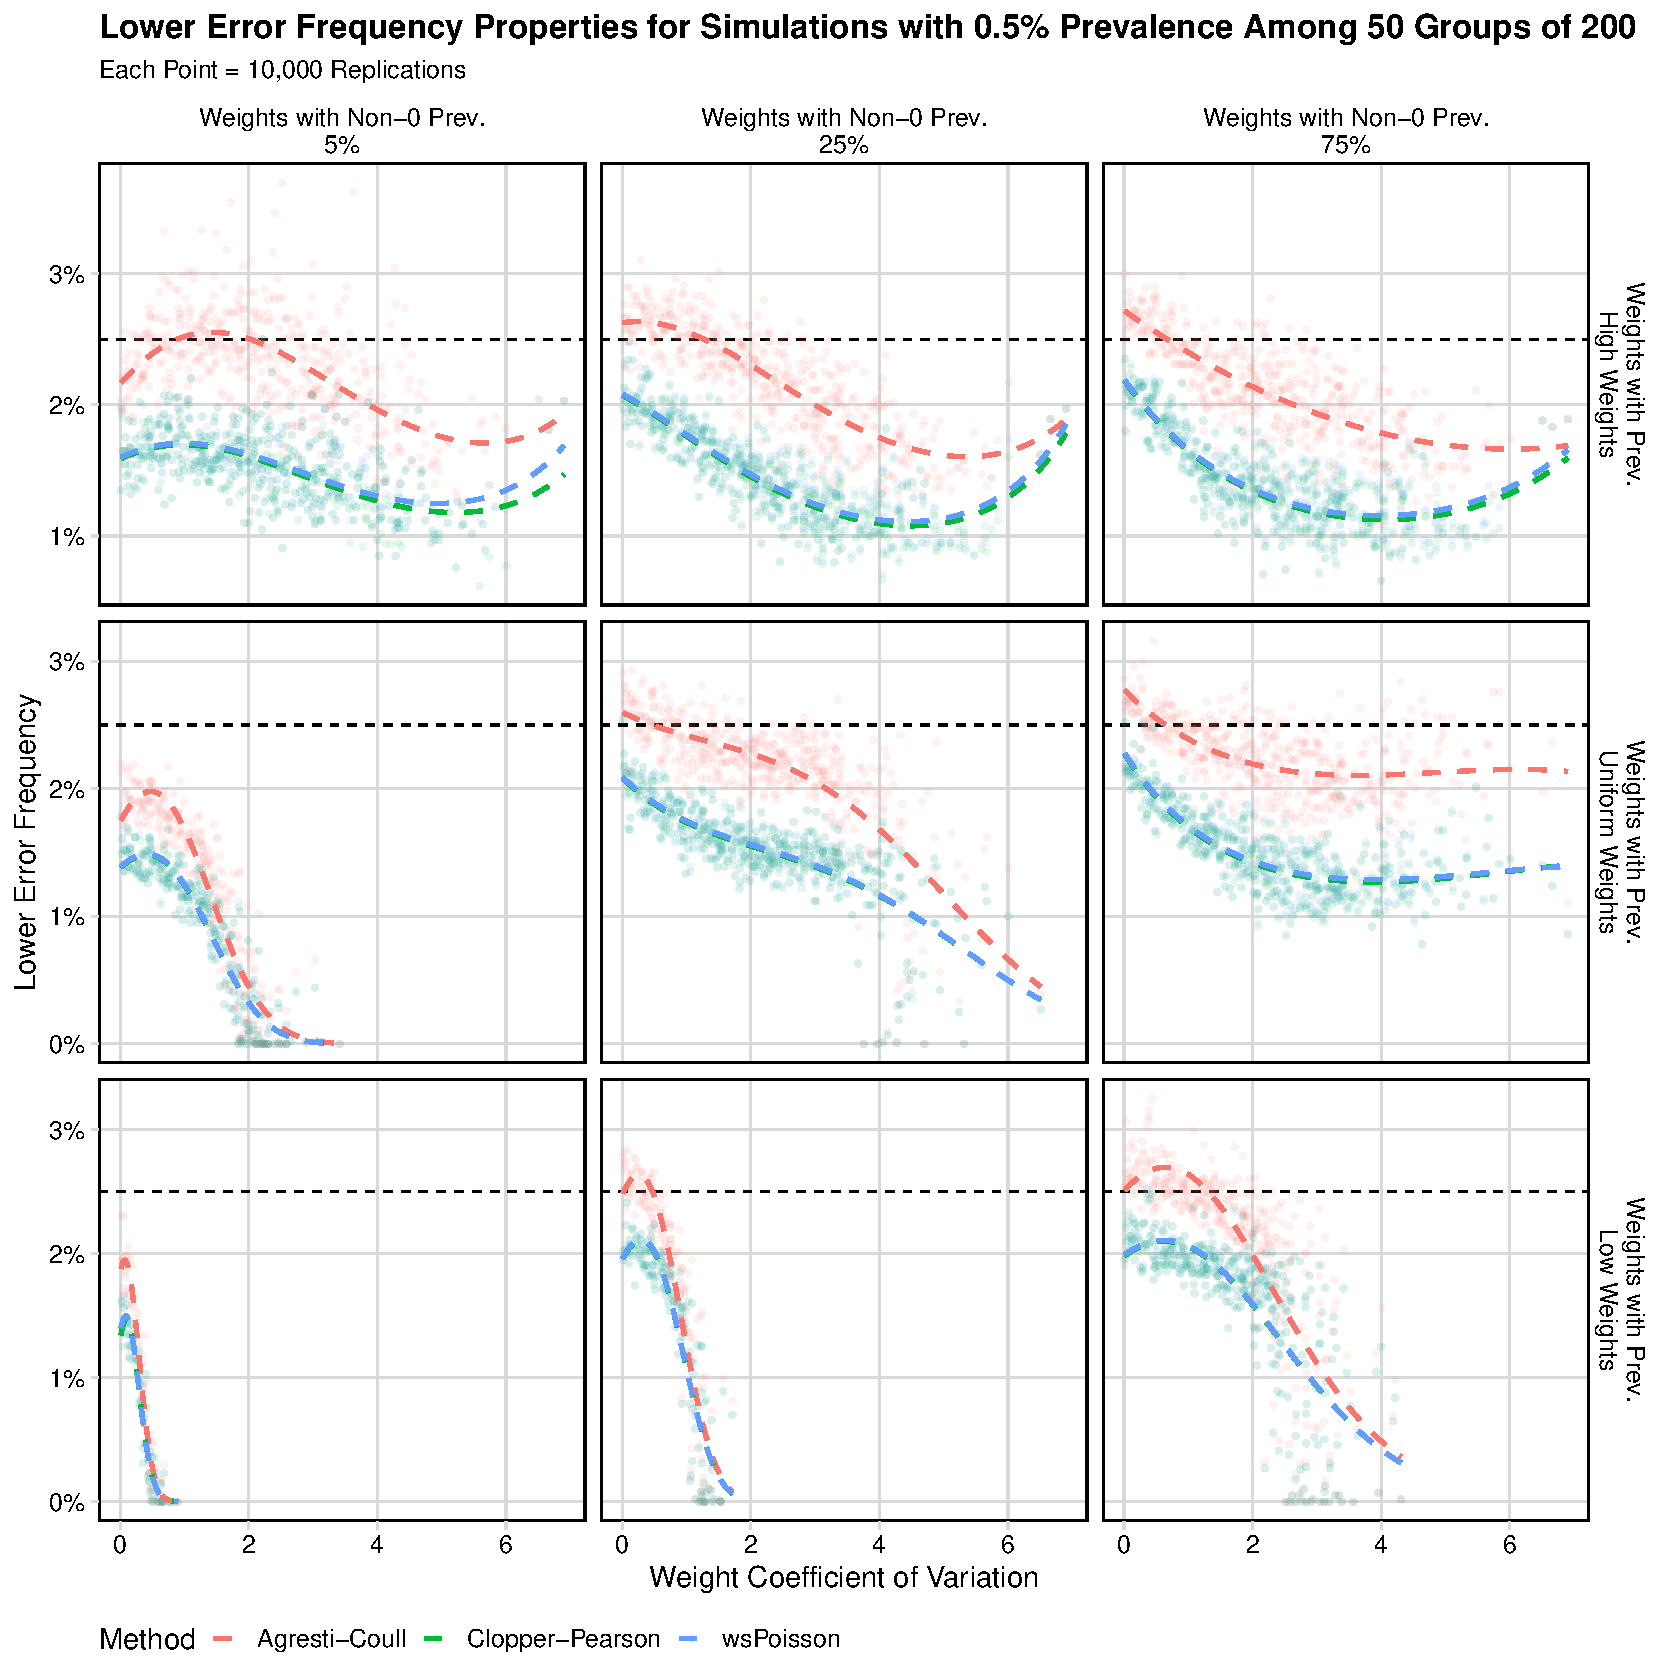
\includegraphics[width=0.8\textwidth]{figures/perfect_lower_error_frequency_50_groups_0_005_prev.pdf}
\caption{Lower error properties for the wsPoisson model and two standard methods, Agresti-Coull and Clopper-Pearson.
Each point represents 10,000 simulations of datasets from a population with 0.5\% Prevalence where 50 groups of 200 people are sampled.
The horizontal dashed line indicates the nominal lower error rate, 2.5\%.
Colored dashed lines are estimates from a logistic regression model using cubic splines.}
\label{fig:perfect_lower_error_frequency_50_groups_0_005_prev}
\end{figure}

\begin{figure}
\centering
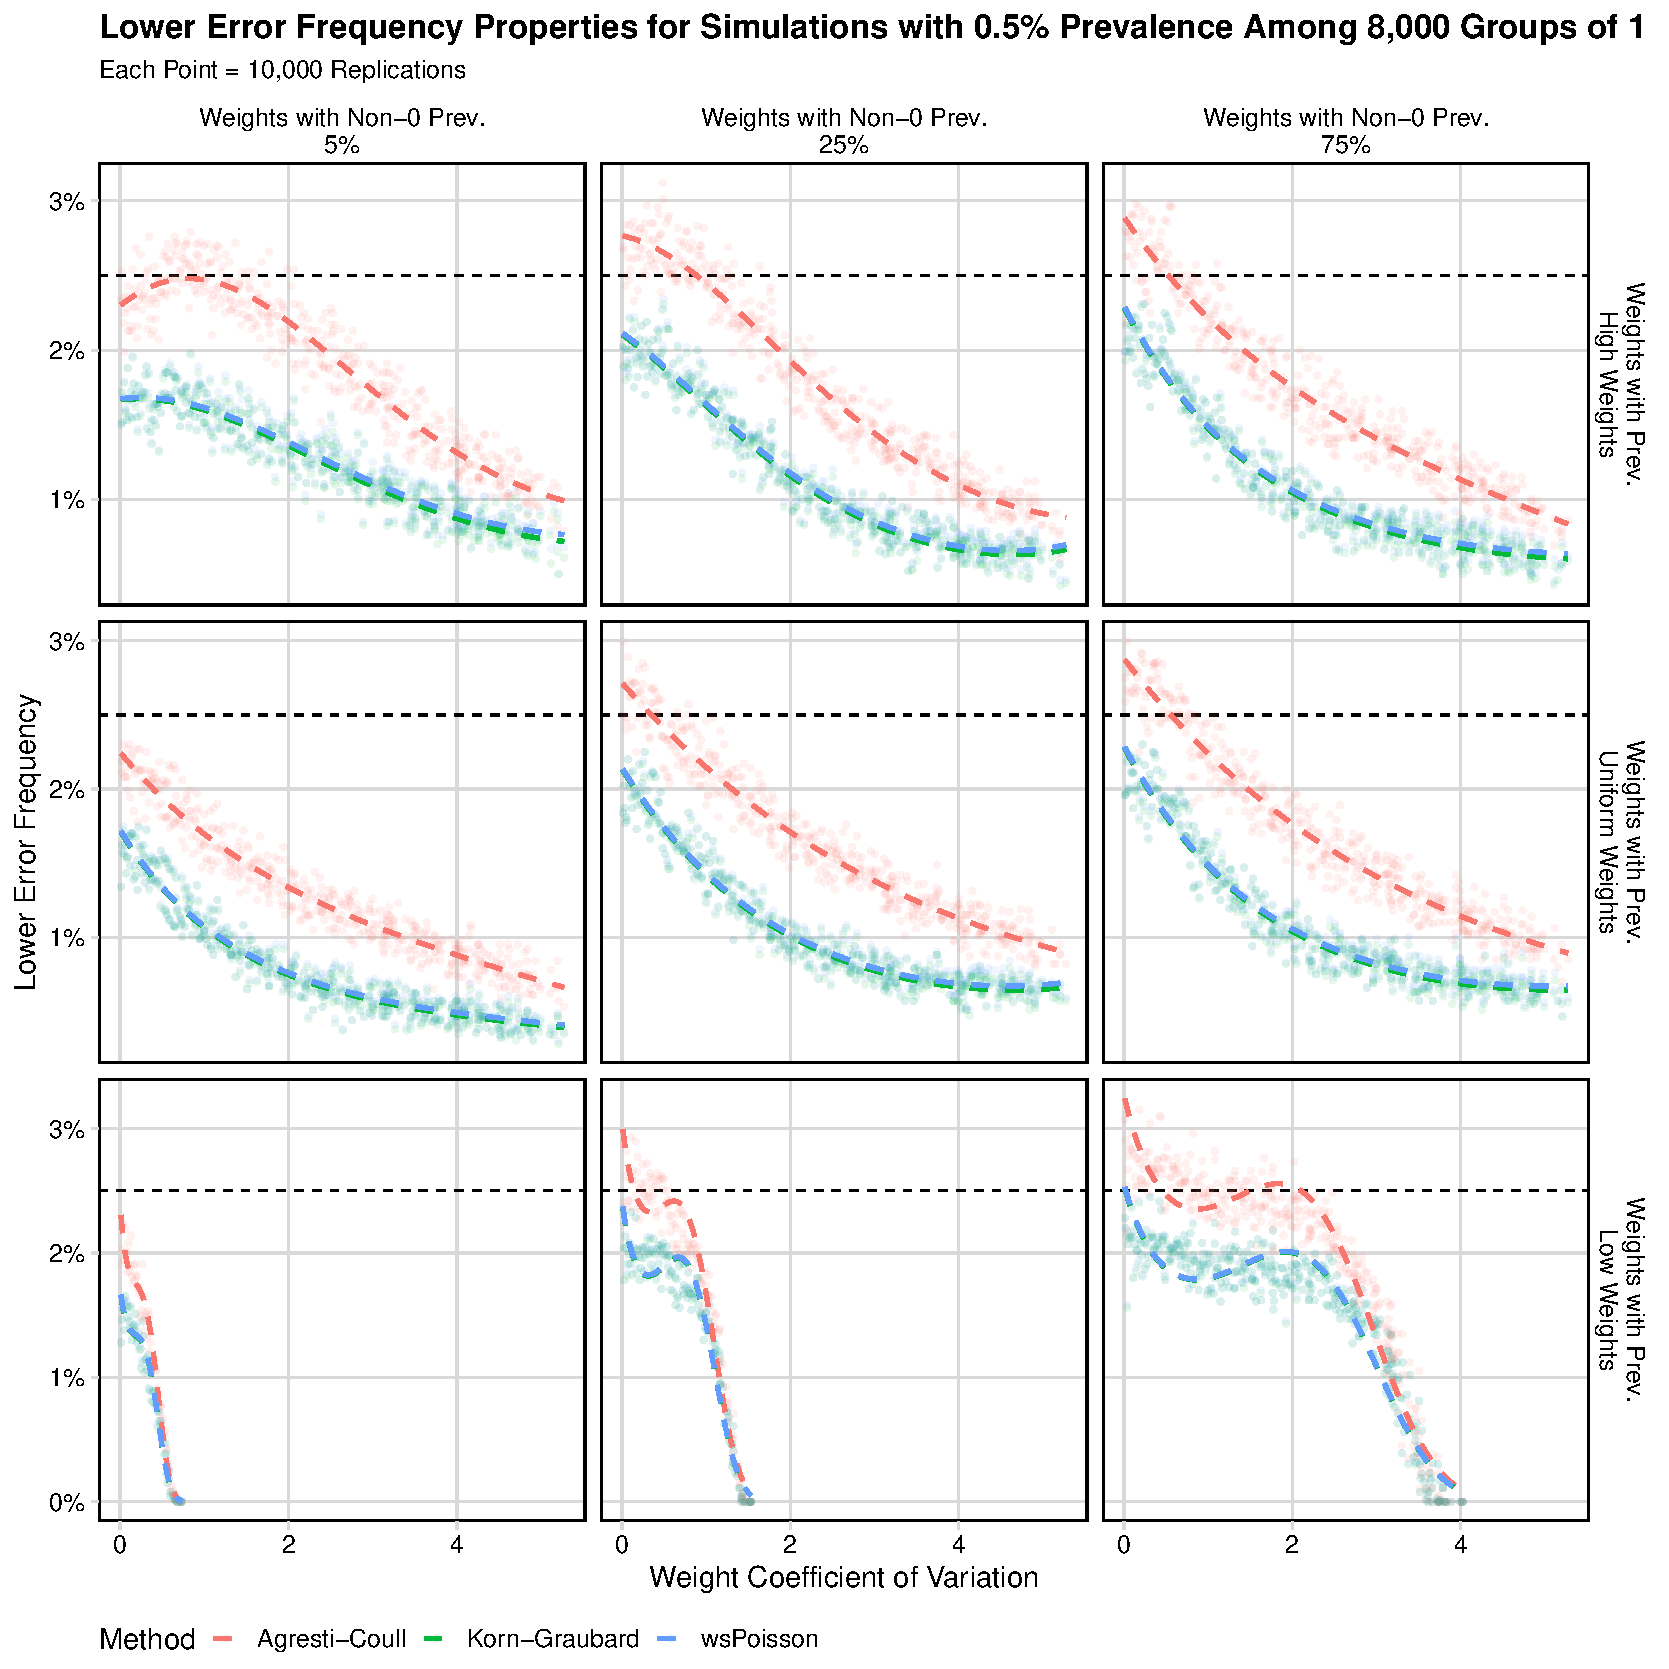
\includegraphics[width=0.8\textwidth]{figures/perfect_lower_error_frequency_8000_groups_0_005_prev.pdf}
\caption{Lower error properties for the wsPoisson model and two standard methods, Agresti-Coull and Clopper-Pearson.
Each point represents 10,000 simulations of datasets from a population with 0.5\% Prevalence where 8000 individuals are sampled.
The horizontal dashed line indicates the nominal lower error rate, 2.5\%.
Colored dashed lines are estimates from a logistic regression model using cubic splines.}
\label{fig:perfect_lower_error_frequency_8000_groups_0_005_prev}
\end{figure}

\begin{figure}
\centering
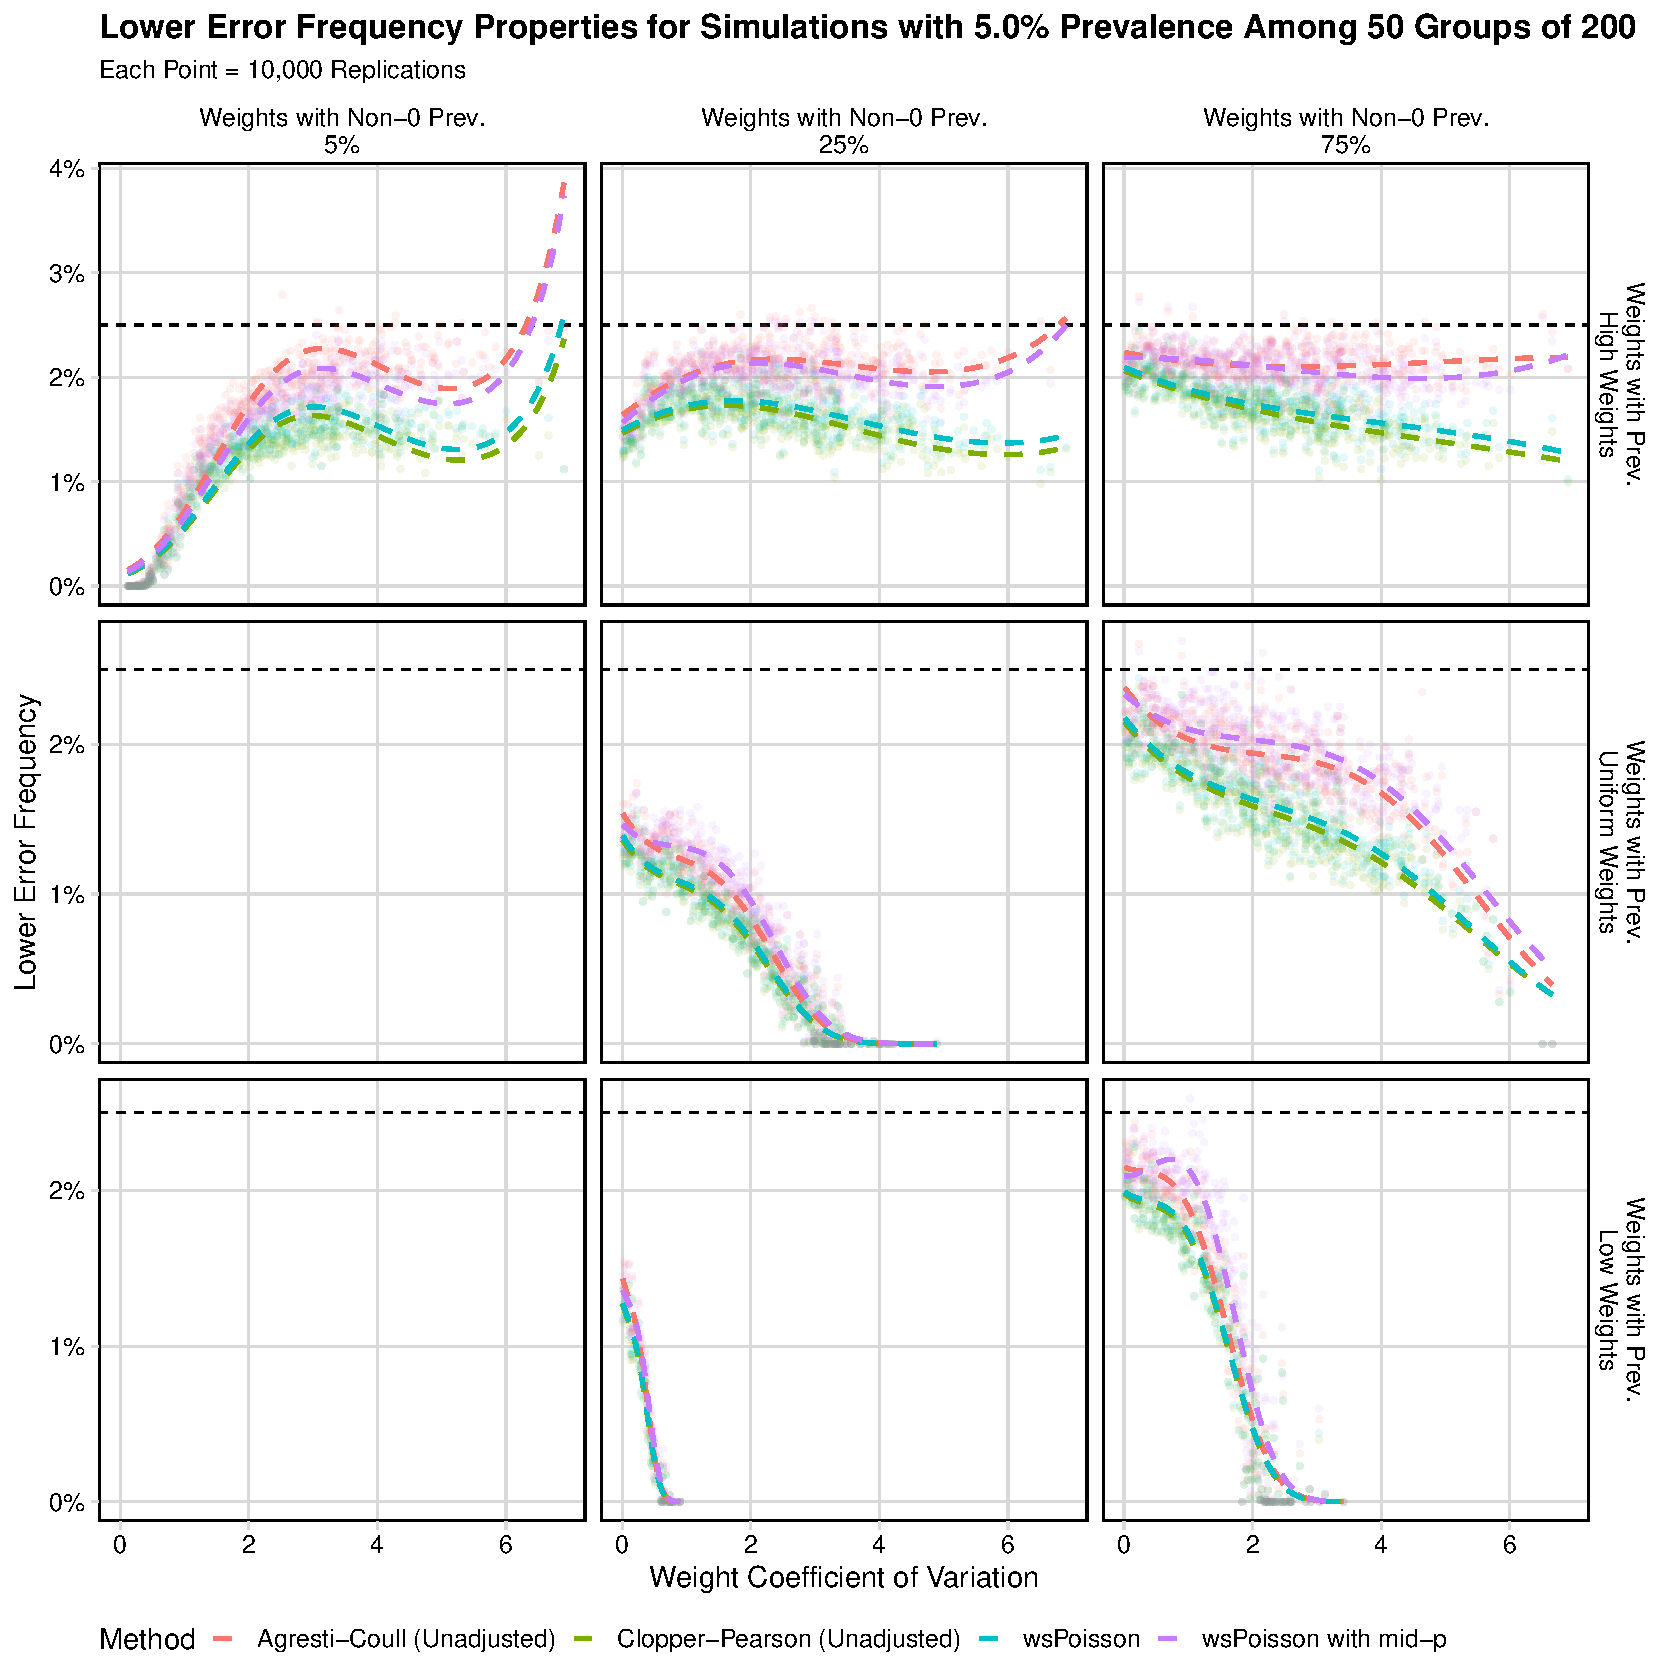
\includegraphics[width=0.8\textwidth]{figures/perfect_lower_error_frequency_50_groups_0_05_prev.pdf}
\caption{Lower error properties for the wsPoisson model and two standard methods, Agresti-Coull and Clopper-Pearson.
Each point represents 10,000 simulations of datasets from a population with 5\% Prevalence where 50 groups of 200 people are sampled.
The horizontal dashed line indicates the nominal lower error rate, 2.5\%.
Colored dashed lines are estimates from a logistic regression model using cubic splines.}
\label{fig:perfect_lower_error_frequency_50_groups_0_05_prev}
\end{figure}

\begin{figure}
\centering
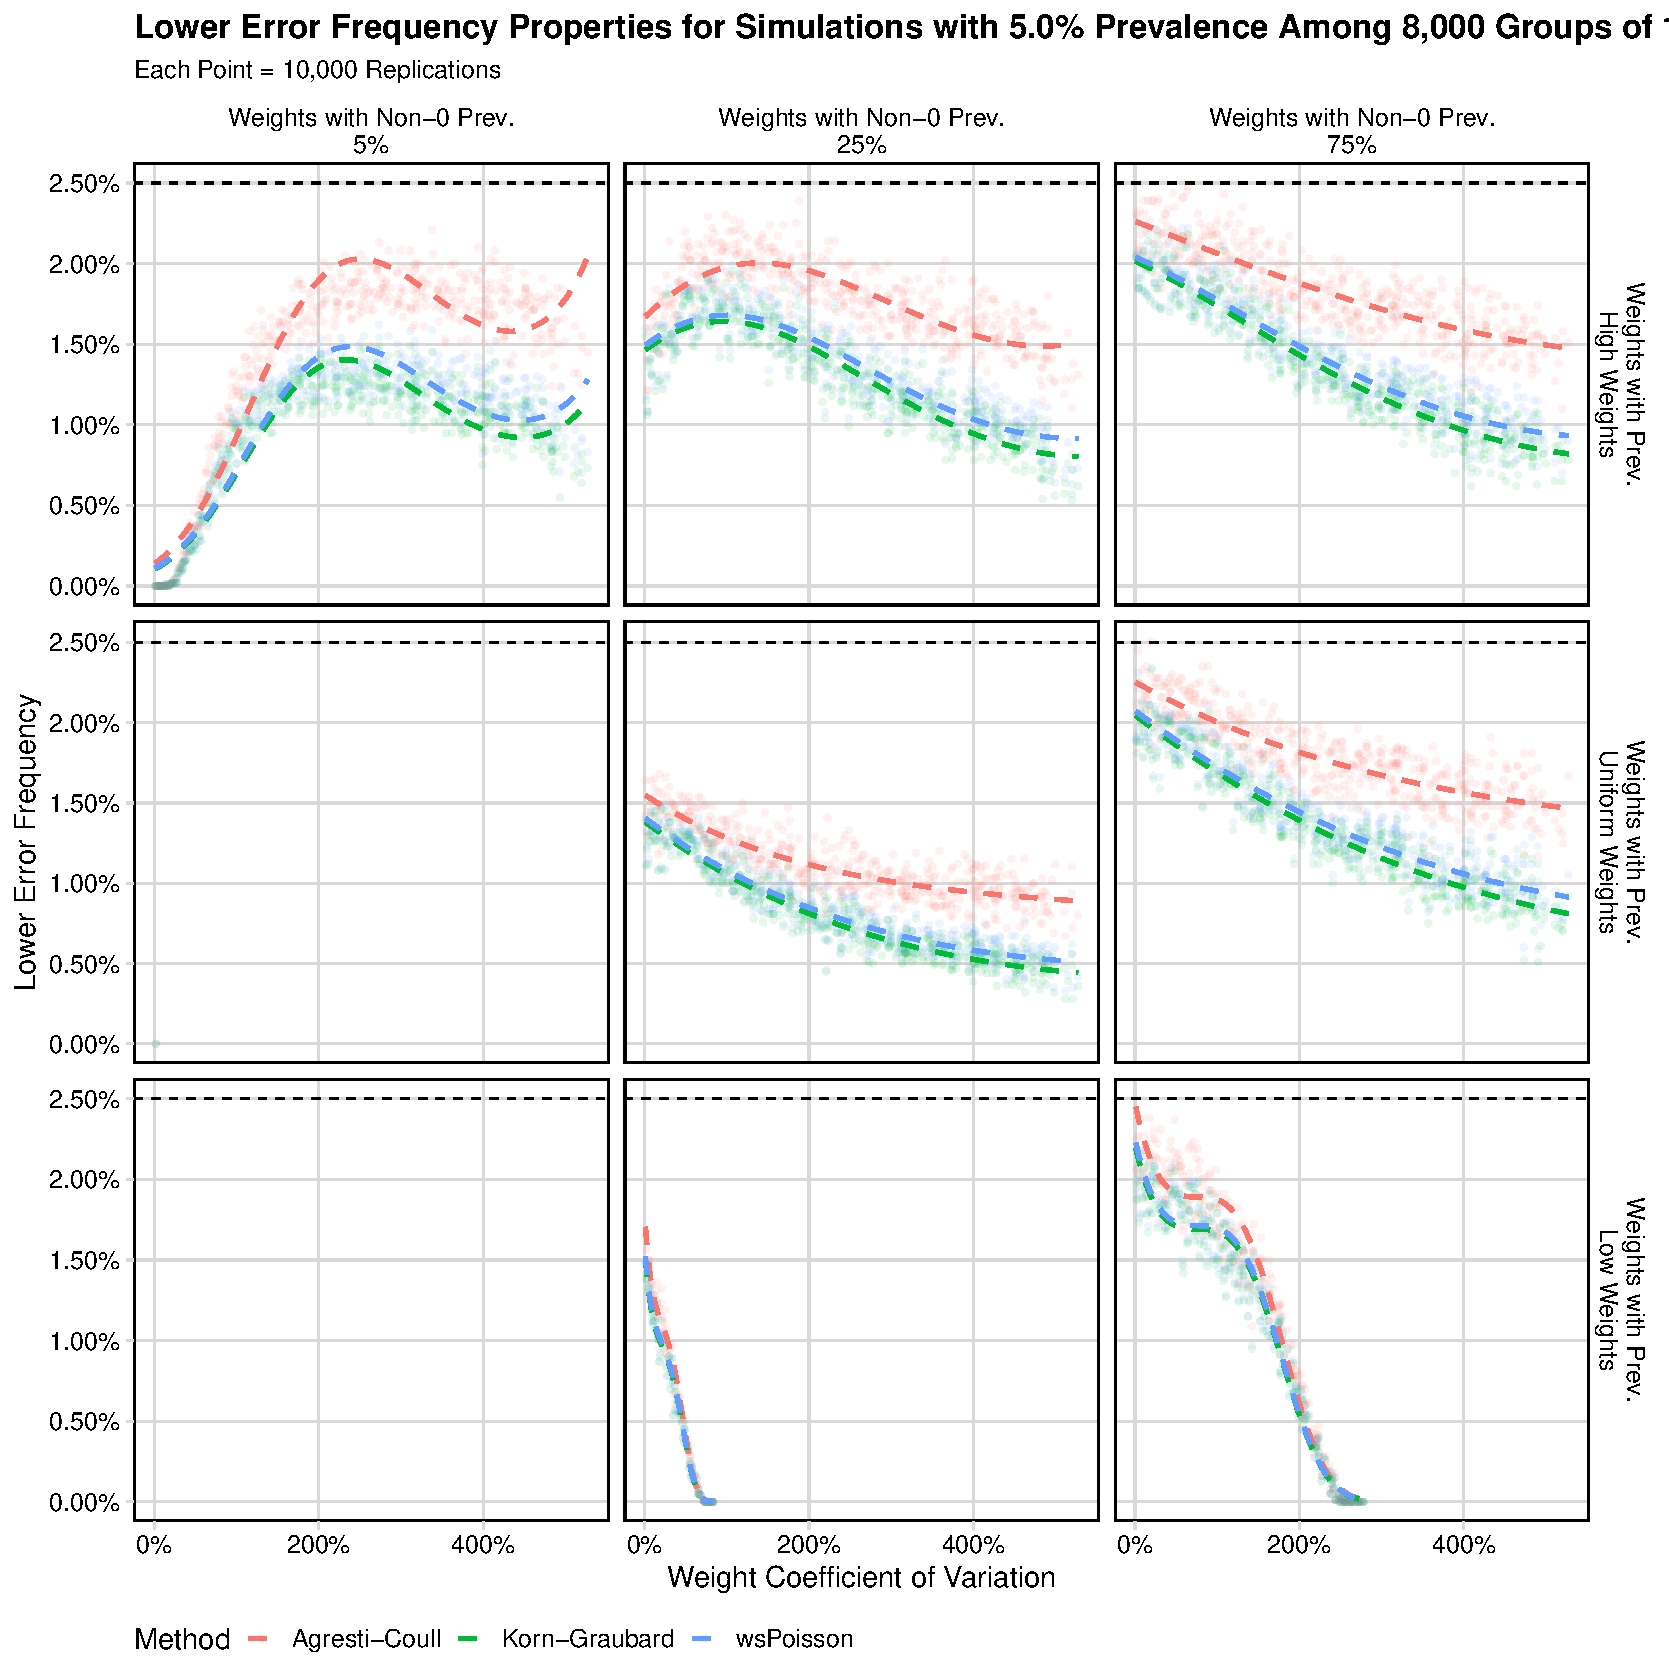
\includegraphics[width=0.8\textwidth]{figures/perfect_lower_error_frequency_8000_groups_0_05_prev.pdf}
\caption{Lower error properties for the wsPoisson model and two standard methods, Agresti-Coull and Clopper-Pearson.
Each point represents 10,000 simulations of datasets from a population with 5\% Prevalence where 8000 individuals are sampled.
The horizontal dashed line indicates the nominal lower error rate, 2.5\%.
Colored dashed lines are estimates from a logistic regression model using cubic splines.}
\label{fig:perfect_lower_error_frequency_8000_groups_0_05_prev}
\end{figure}

\begin{figure}
\centering
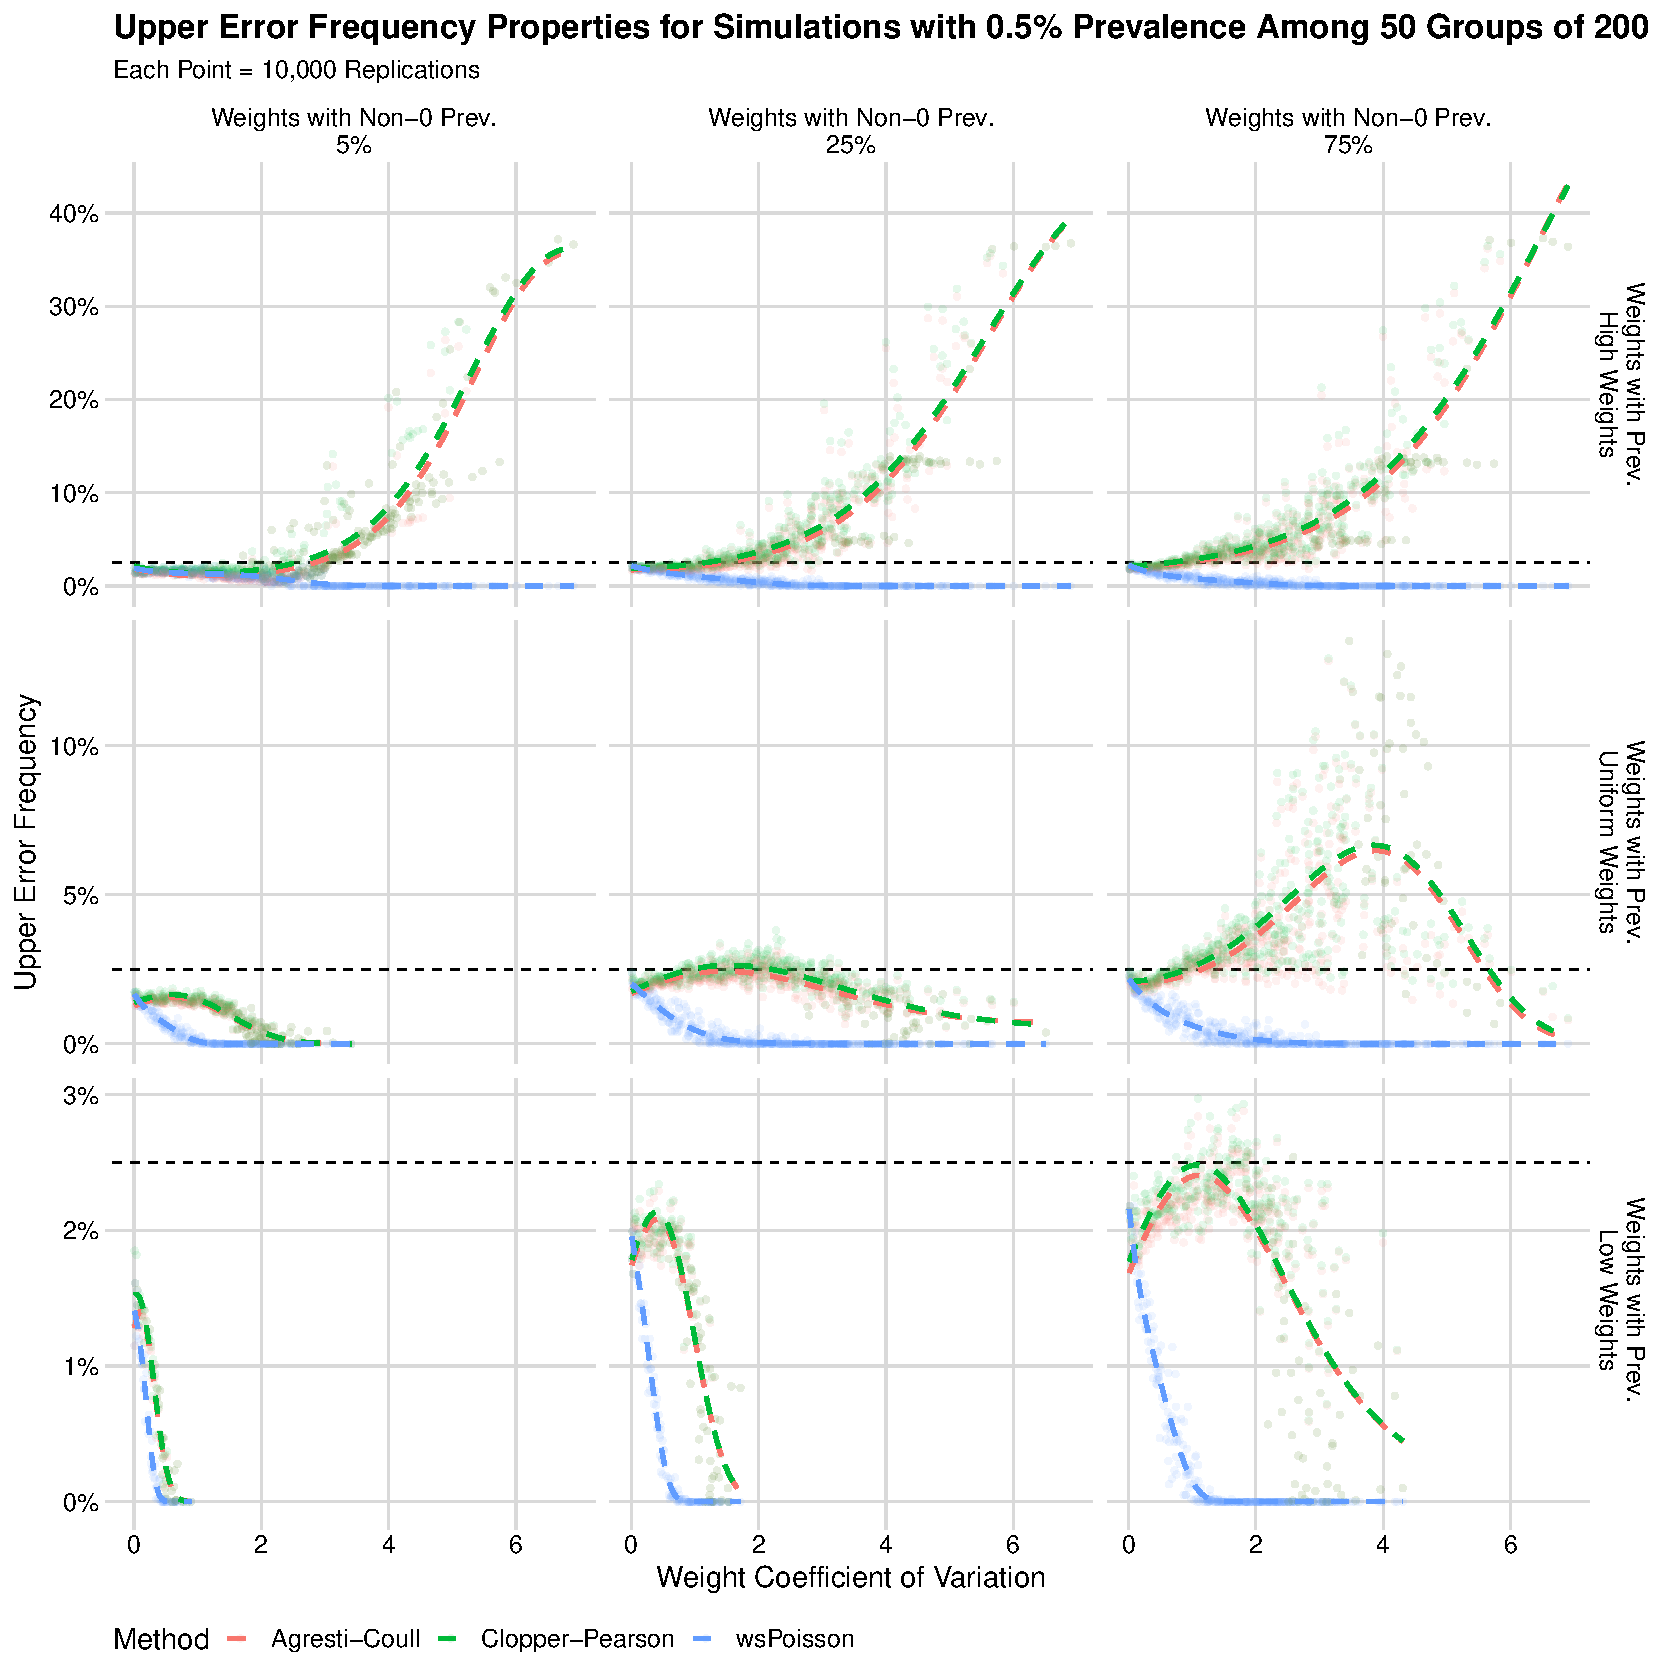
\includegraphics[width=0.8\textwidth]{figures/perfect_upper_error_frequency_50_groups_0_005_prev.pdf}
\caption{Upper error properties for the wsPoisson model and two standard methods, Agresti-Coull and Clopper-Pearson.
Each point represents 10,000 simulations of datasets from a population with 0.5\% Prevalence where 50 groups of 200 people are sampled.
The horizontal dashed line indicates the nominal upper error rate, 2.5\%.
Colored dashed lines are estimates from a logistic regression model using cubic splines.}
\label{fig:perfect_upper_error_frequency_50_groups_0_005_prev}
\end{figure}

\begin{figure}
\centering
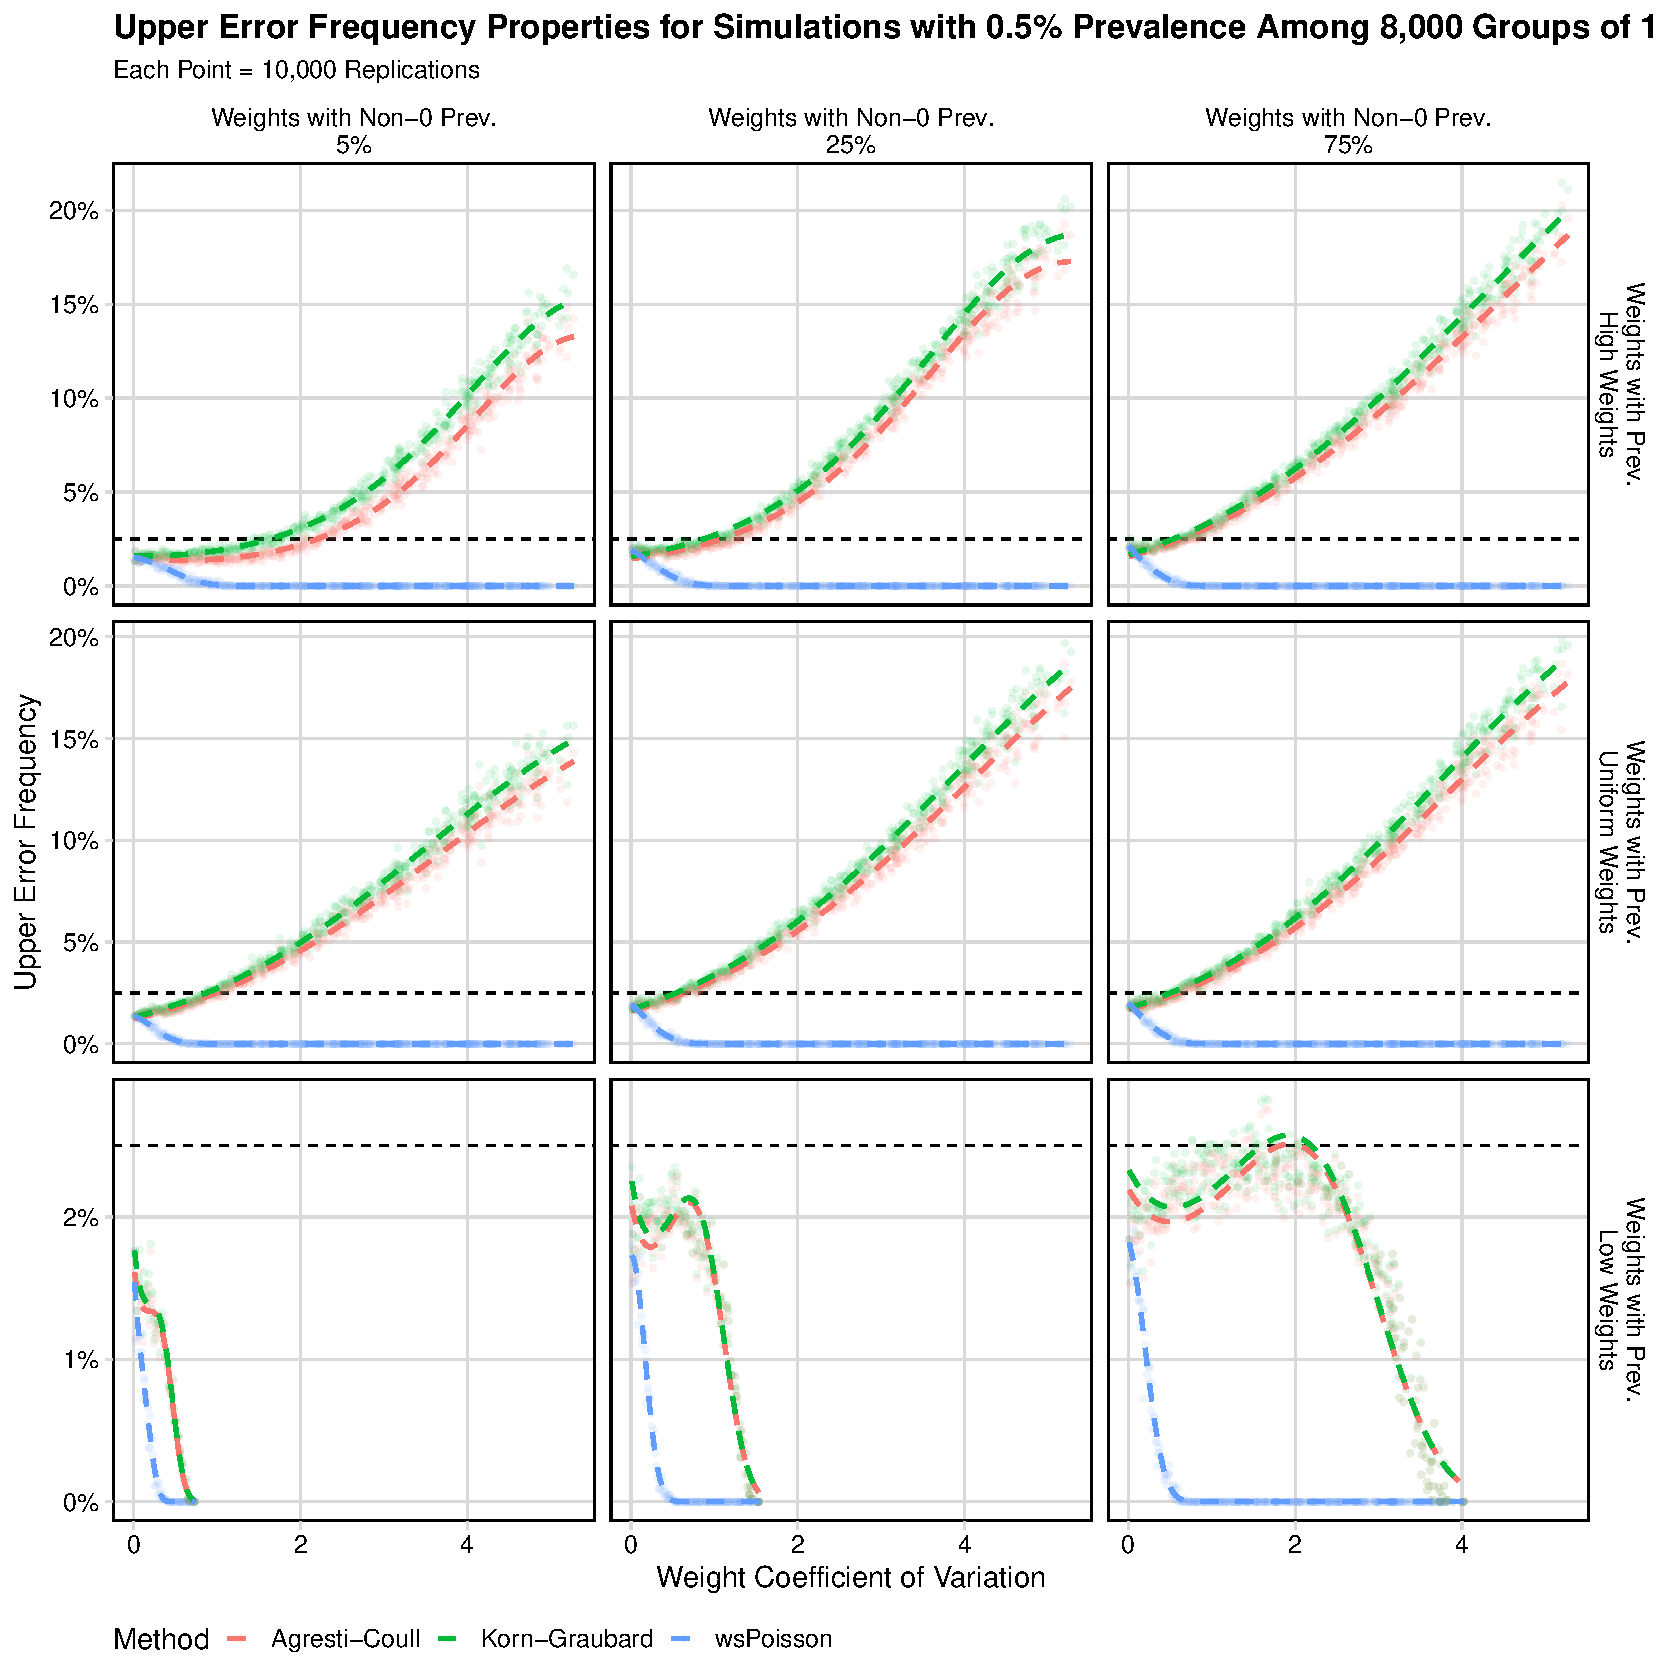
\includegraphics[width=0.8\textwidth]{figures/perfect_upper_error_frequency_8000_groups_0_005_prev.pdf}
\caption{Upper error properties for the wsPoisson model and two standard methods, Agresti-Coull and Clopper-Pearson.
Each point represents 10,000 simulations of datasets from a population with 0.5\% Prevalence where 8000 individuals are sampled.
The horizontal dashed line indicates the nominal upper error rate, 2.5\%.
Colored dashed lines are estimates from a logistic regression model using cubic splines.}
\label{fig:perfect_upper_error_frequency_8000_groups_0_005_prev}
\end{figure}

\begin{figure}
\centering
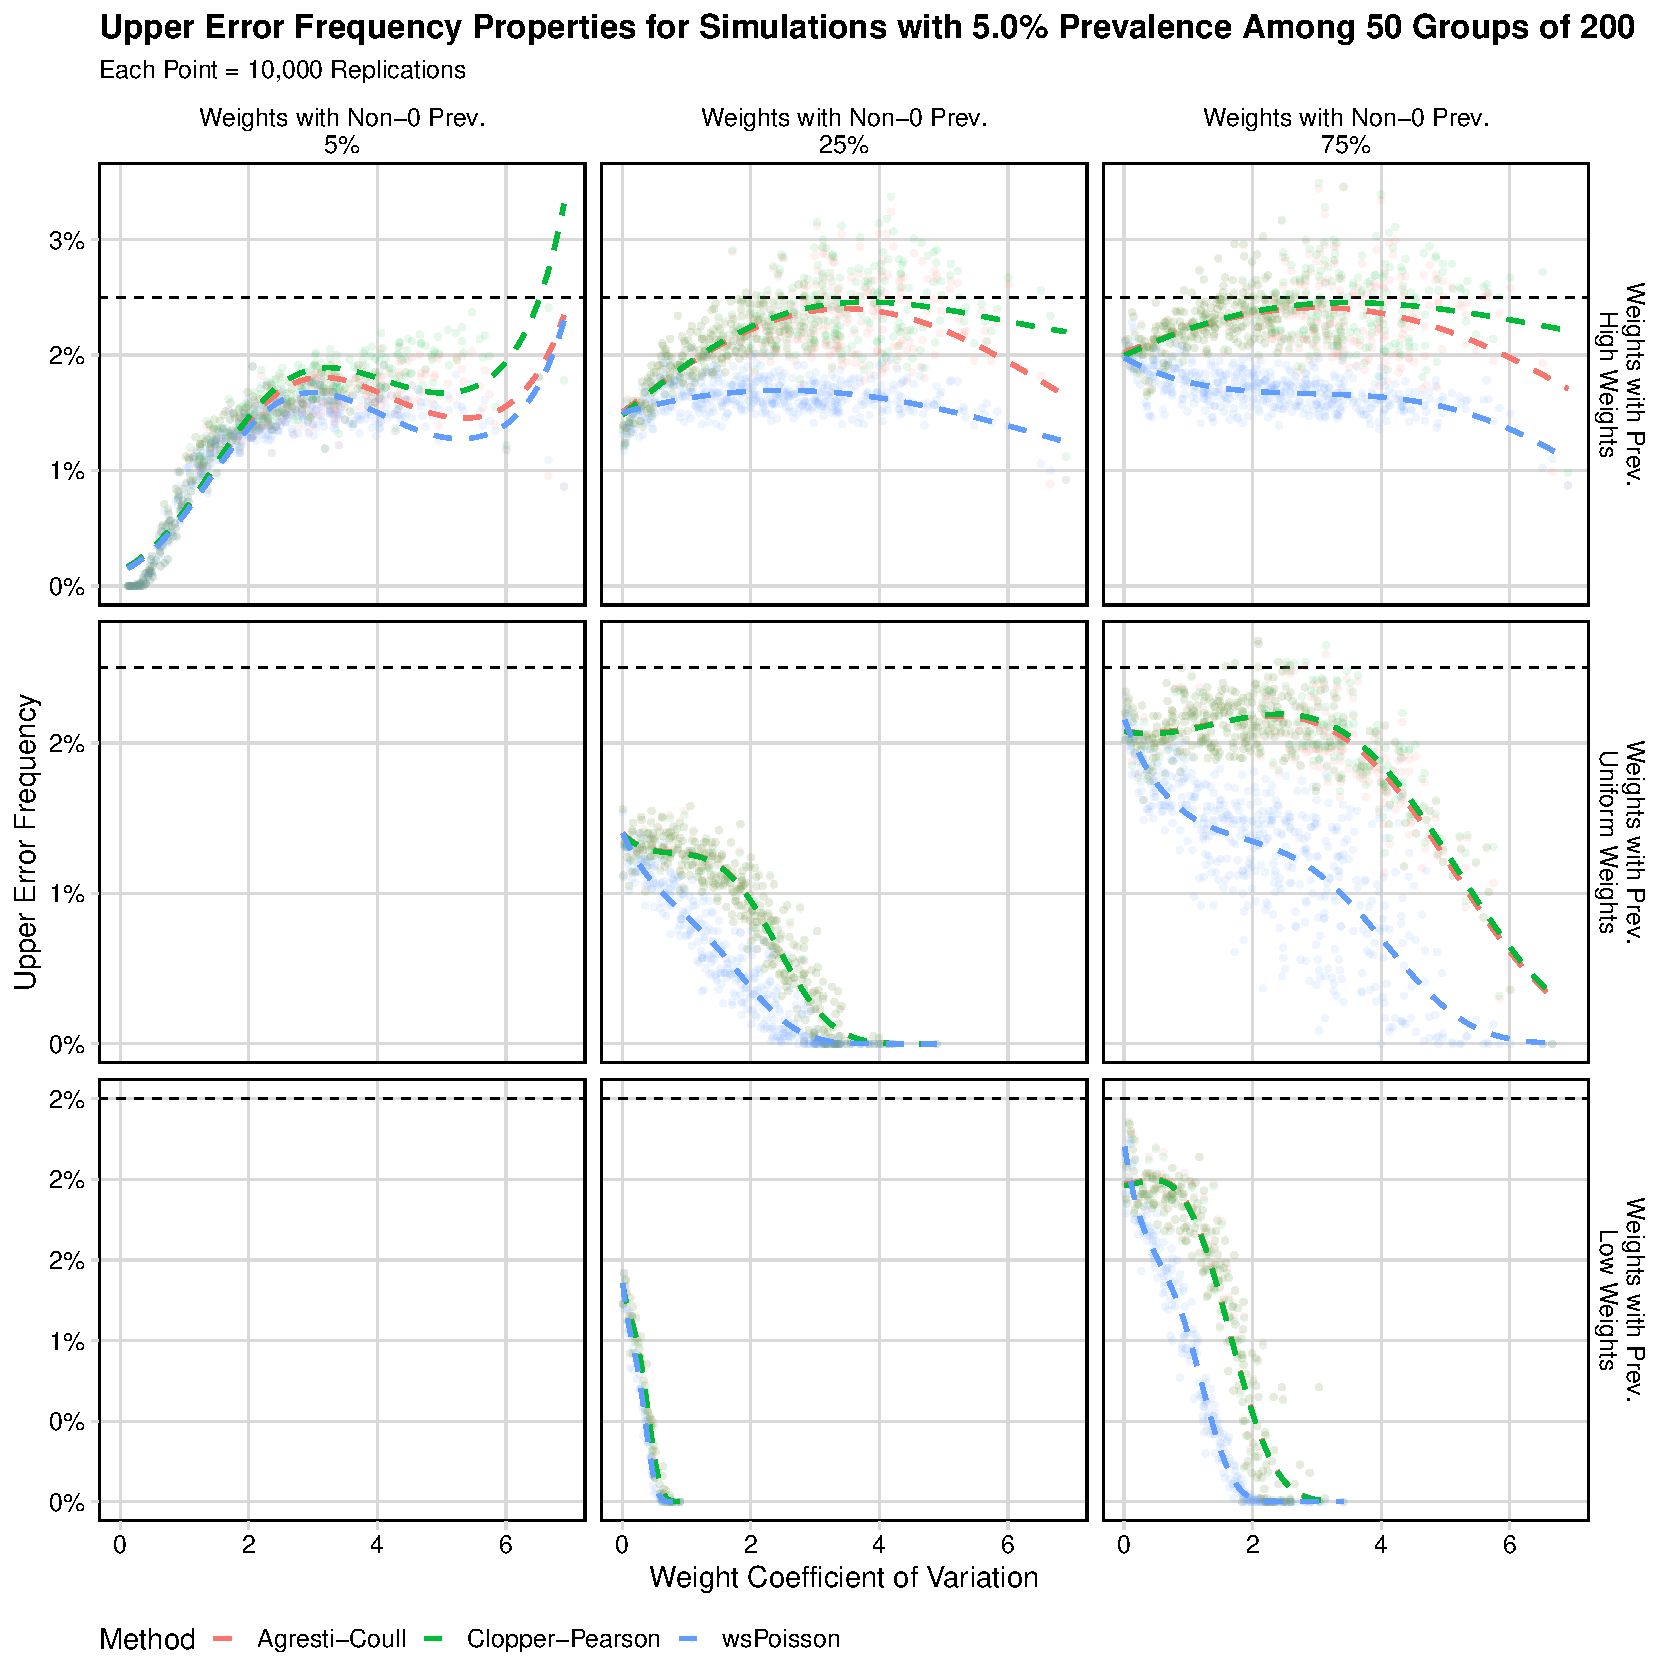
\includegraphics[width=0.8\textwidth]{figures/perfect_upper_error_frequency_50_groups_0_05_prev.pdf}
\caption{Upper error properties for the wsPoisson model and two standard methods, Agresti-Coull and Clopper-Pearson.
Each point represents 10,000 simulations of datasets from a population with 5\% Prevalence where 50 groups of 200 people are sampled.
The horizontal dashed line indicates the nominal upper error rate, 2.5\%.
Colored dashed lines are estimates from a logistic regression model using cubic splines.}
\label{fig:perfect_upper_error_frequency_50_groups_0_05_prev}
\end{figure}

\begin{figure}
\centering
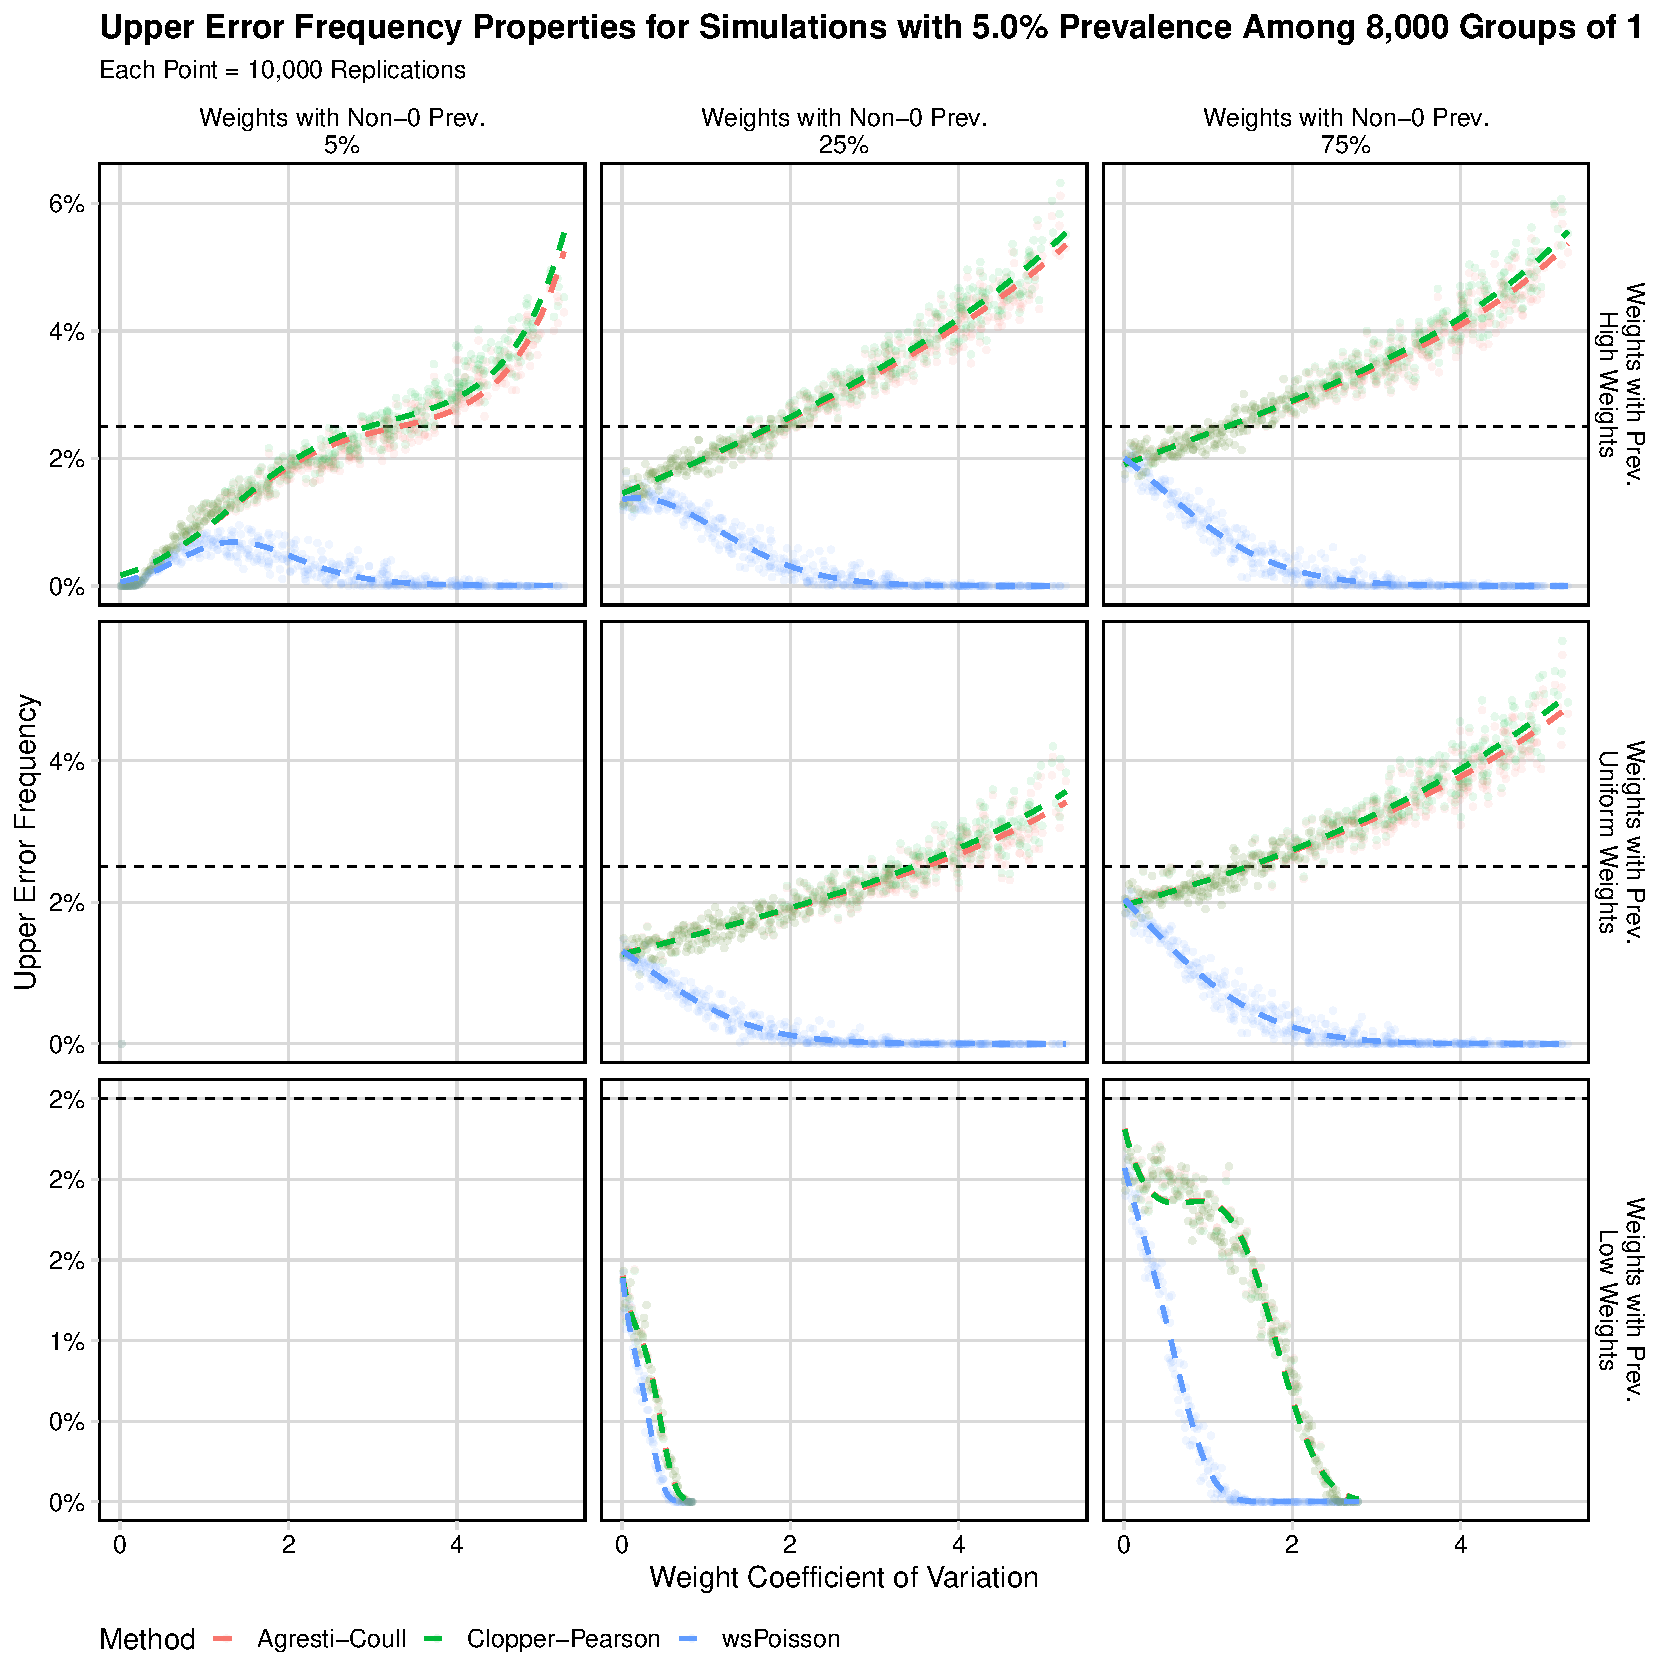
\includegraphics[width=0.8\textwidth]{figures/perfect_upper_error_frequency_8000_groups_0_05_prev.pdf}
\caption{Upper error properties for the wsPoisson model and two standard methods, Agresti-Coull and Clopper-Pearson.
Each point represents 10,000 simulations of datasets from a population with 5\% Prevalence where 8000 individuals are sampled.
The horizontal dashed line indicates the nominal upper error rate, 2.5\%.
Colored dashed lines are estimates from a logistic regression model using cubic splines.}
\label{fig:perfect_upper_error_frequency_8000_groups_0_05_prev}
\end{figure}

% Start of Imperfect

\begin{figure}
\centering
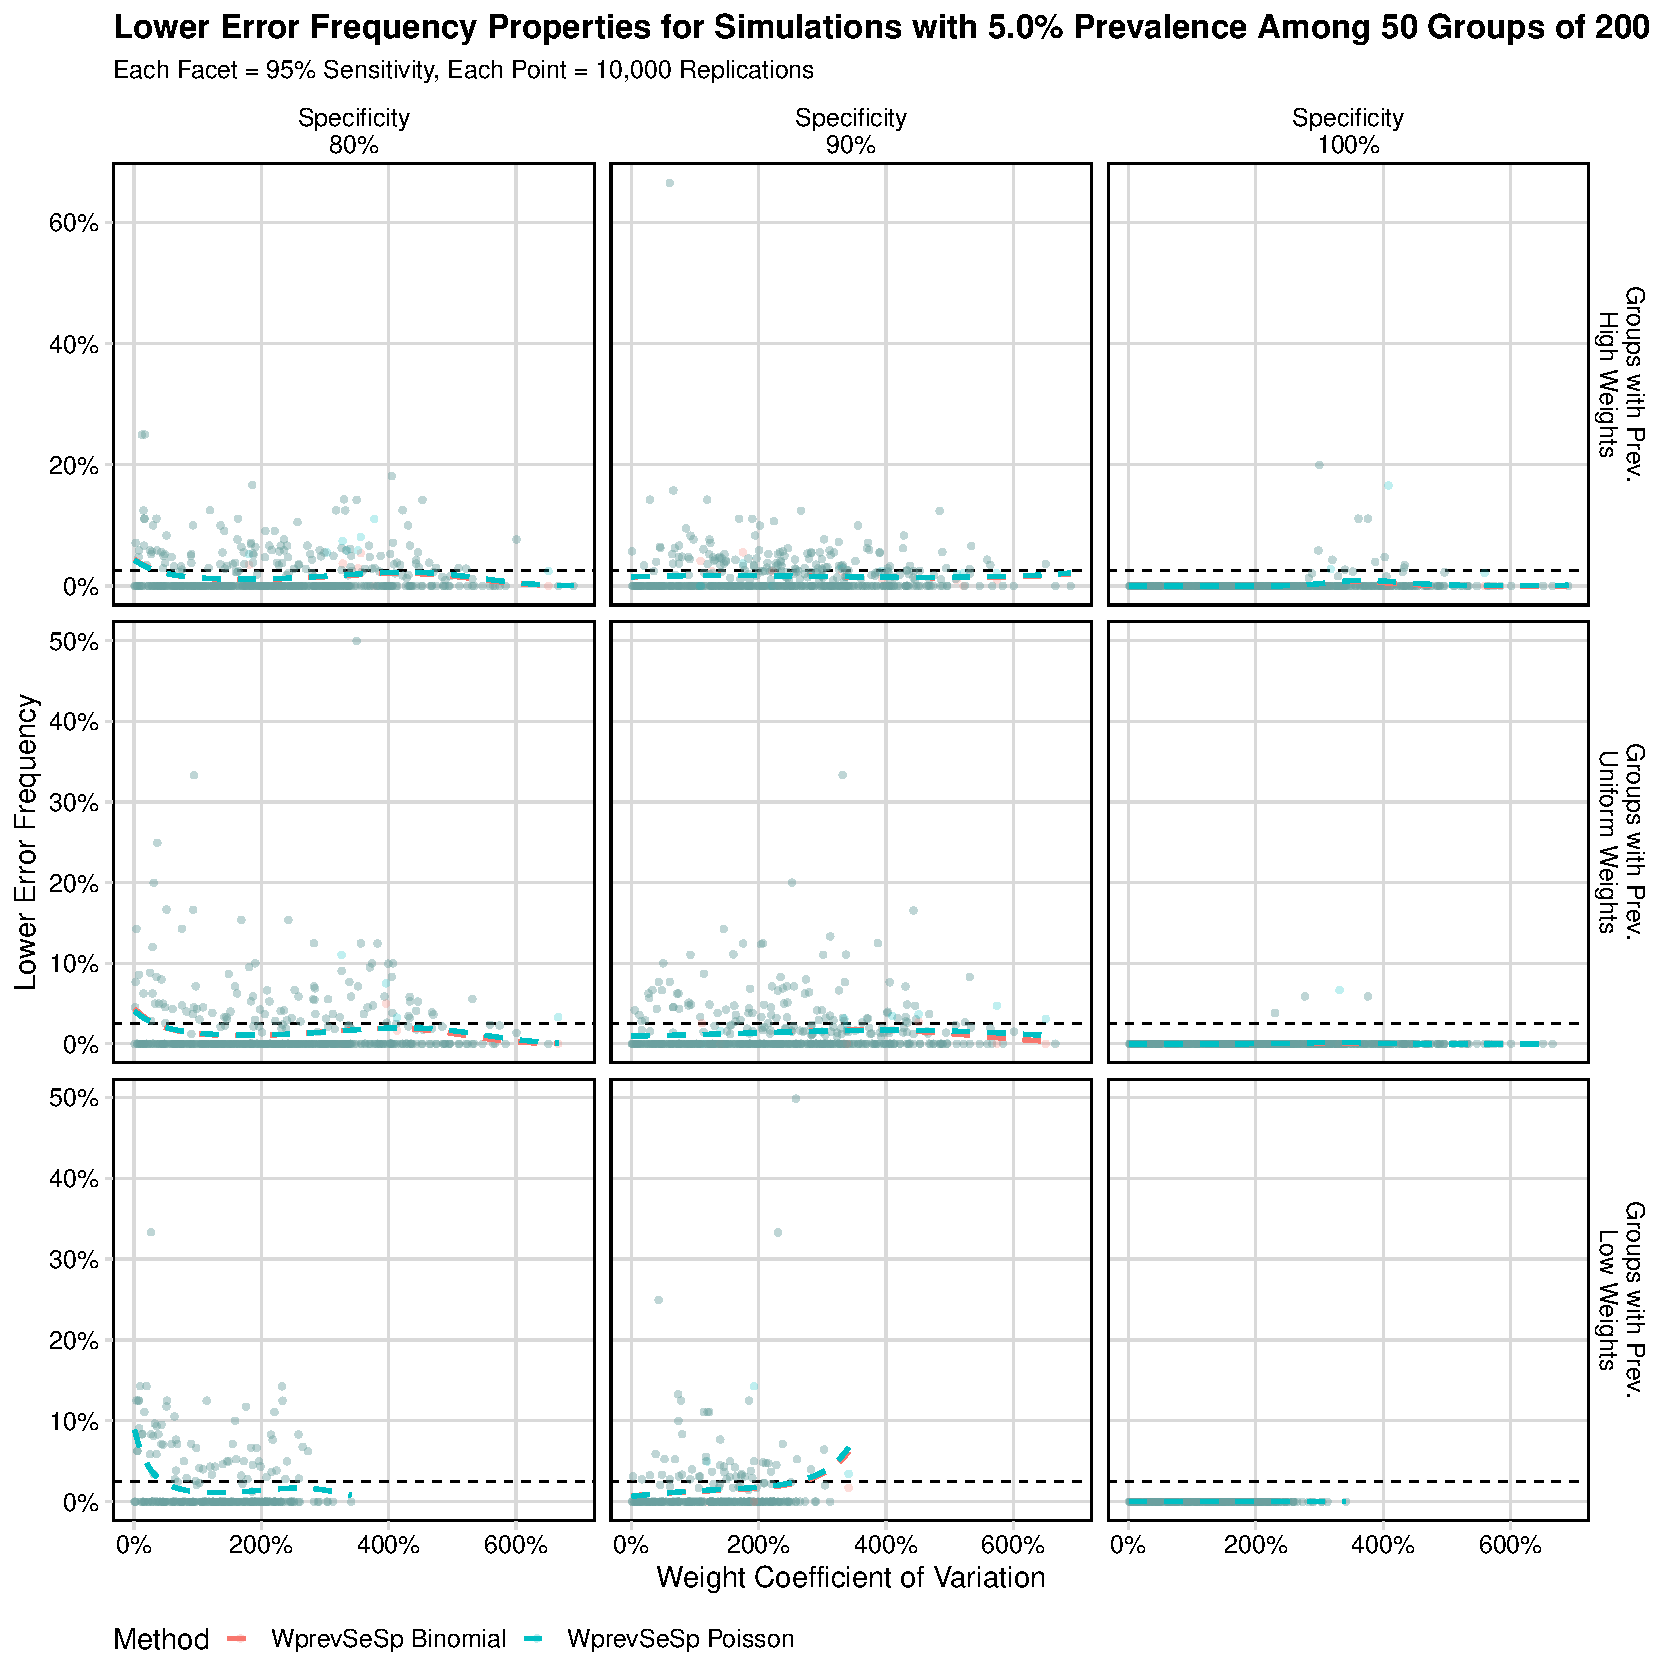
\includegraphics[width=0.8\textwidth]{figures/imperfect_lower_error_frequency_50_groups_0_05_prev.pdf}
\caption{Lower error properties for the two melded confidence interval procedures, WprevSeSp Binomial and WprevSeSp Poisson, and one method, wspoissonTest, which does not account for the imperfect assay.
Each point represents 10,000 simulations of datasets from a population with 0.5\% Prevalence where 50 groups of 200 people are sampled.
Each datasets also includes simulated results of tests to evaluate the sensitivity and specificity of the assay performed on 60 and 300 individuals, respectively.
The horizontal dashed line indicates the nominal lower error rate, 2.5\%.
Colored dashed lines are estimates from a logistic regression model using cubic splines.}
\label{fig:imperfect_lower_error_frequency_50_groups_0_05_prev}
\end{figure}

\begin{figure}
\centering
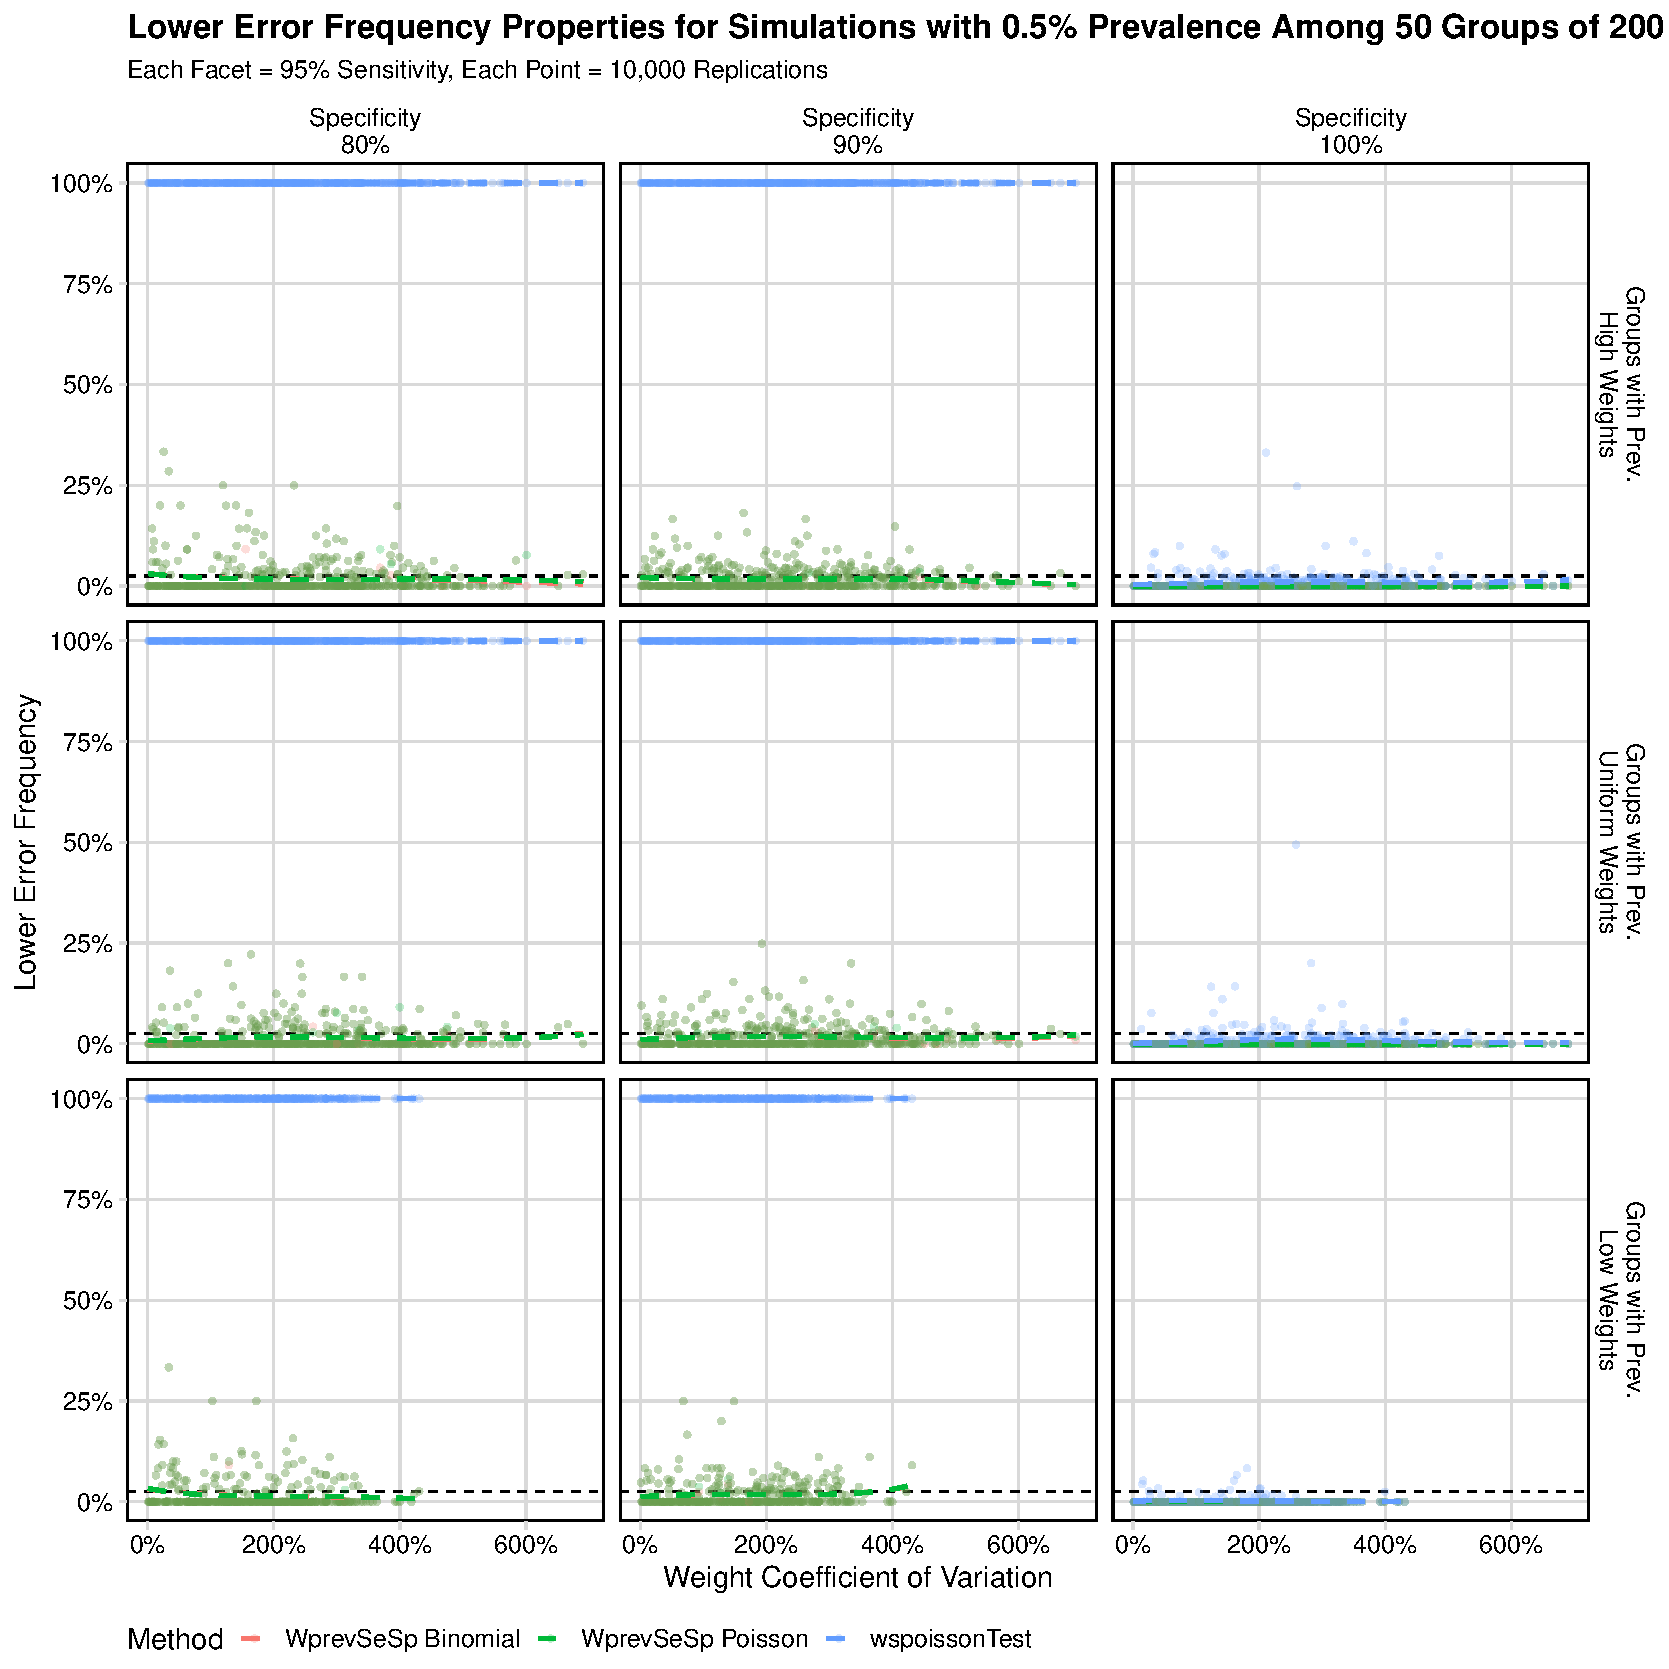
\includegraphics[width=0.8\textwidth]{figures/imperfect_lower_error_frequency_50_groups_0_005_prev.pdf}
\caption{Lower error properties for the two melded confidence interval procedures, WprevSeSp Binomial and WprevSeSp Poisson, and one method, wspoissonTest, which does not account for the imperfect assay.
Each point represents 10,000 simulations of datasets from a population with 0.5\% Prevalence where 8000 individuals are sampled.
Each datasets also includes simulated results of tests to evaluate the sensitivity and specificity of the assay performed on 60 and 300 individuals, respectively.
The horizontal dashed line indicates the nominal lower error rate, 2.5\%.
Colored dashed lines are estimates from a logistic regression model using cubic splines.}
\label{fig:imperfect_lower_error_frequency_50_groups_0_005_prev}
\end{figure}

\begin{figure}
\centering
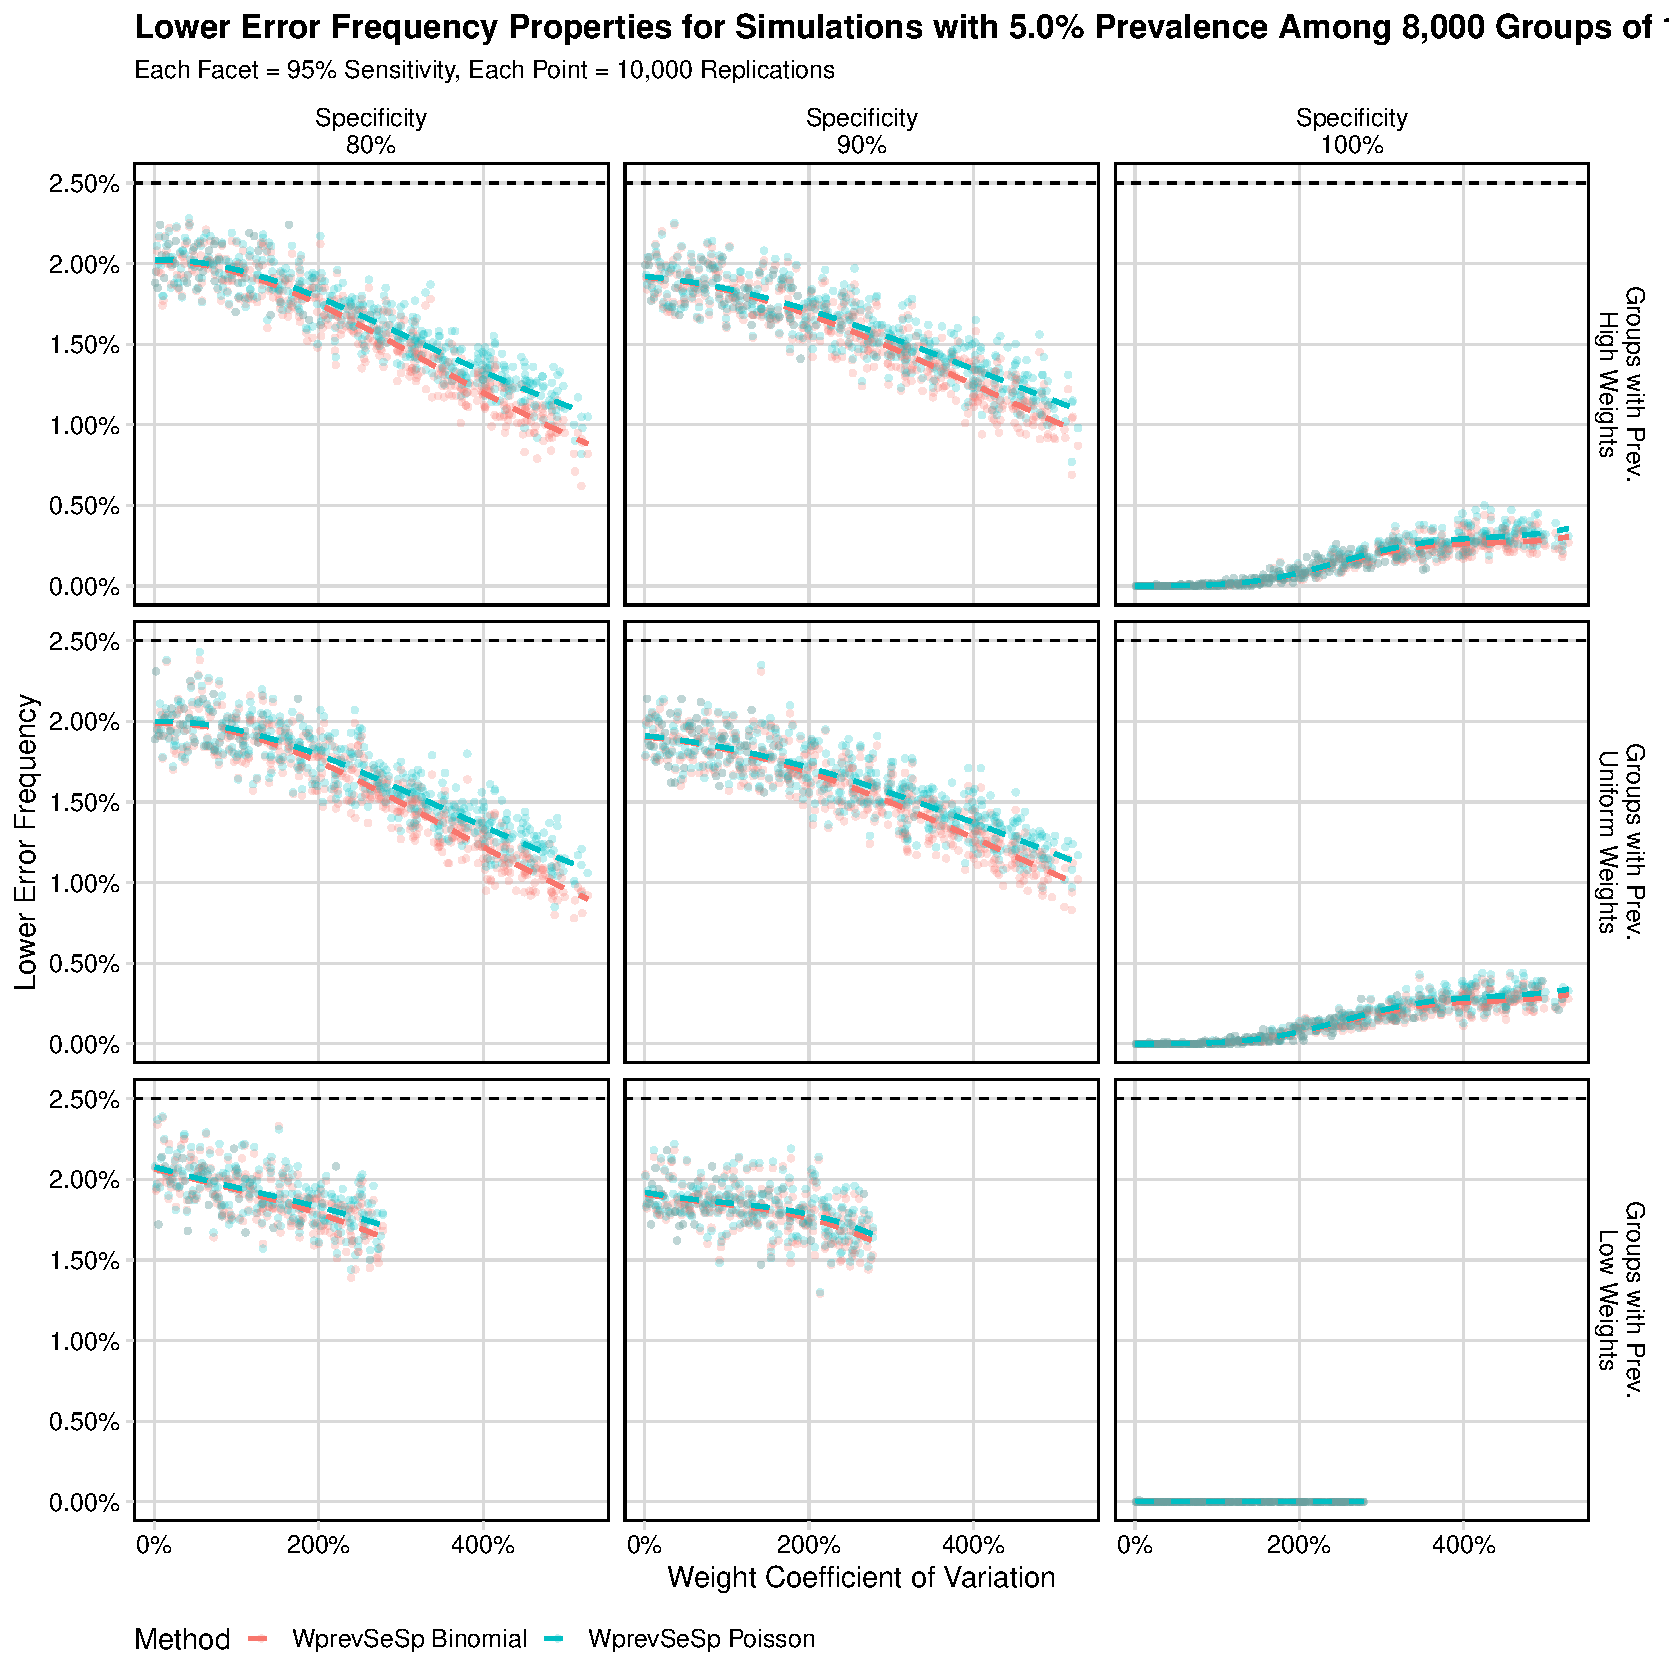
\includegraphics[width=0.8\textwidth]{figures/imperfect_lower_error_frequency_8000_groups_0_05_prev.pdf}
\caption{Lower error properties for the two melded confidence interval procedures, WprevSeSp Binomial and WprevSeSp Poisson, and one method, wspoissonTest, which does not account for the imperfect assay.
Each point represents 10,000 simulations of datasets from a population with 5\% Prevalence where 50 groups of 200 people are sampled.
Each datasets also includes simulated results of tests to evaluate the sensitivity and specificity of the assay performed on 60 and 300 individuals, respectively.
The horizontal dashed line indicates the nominal lower error rate, 2.5\%.
Colored dashed lines are estimates from a logistic regression model using cubic splines.}
\label{fig:imperfect_lower_error_frequency_8000_groups_0_05_prev}
\end{figure}

\begin{figure}
\centering
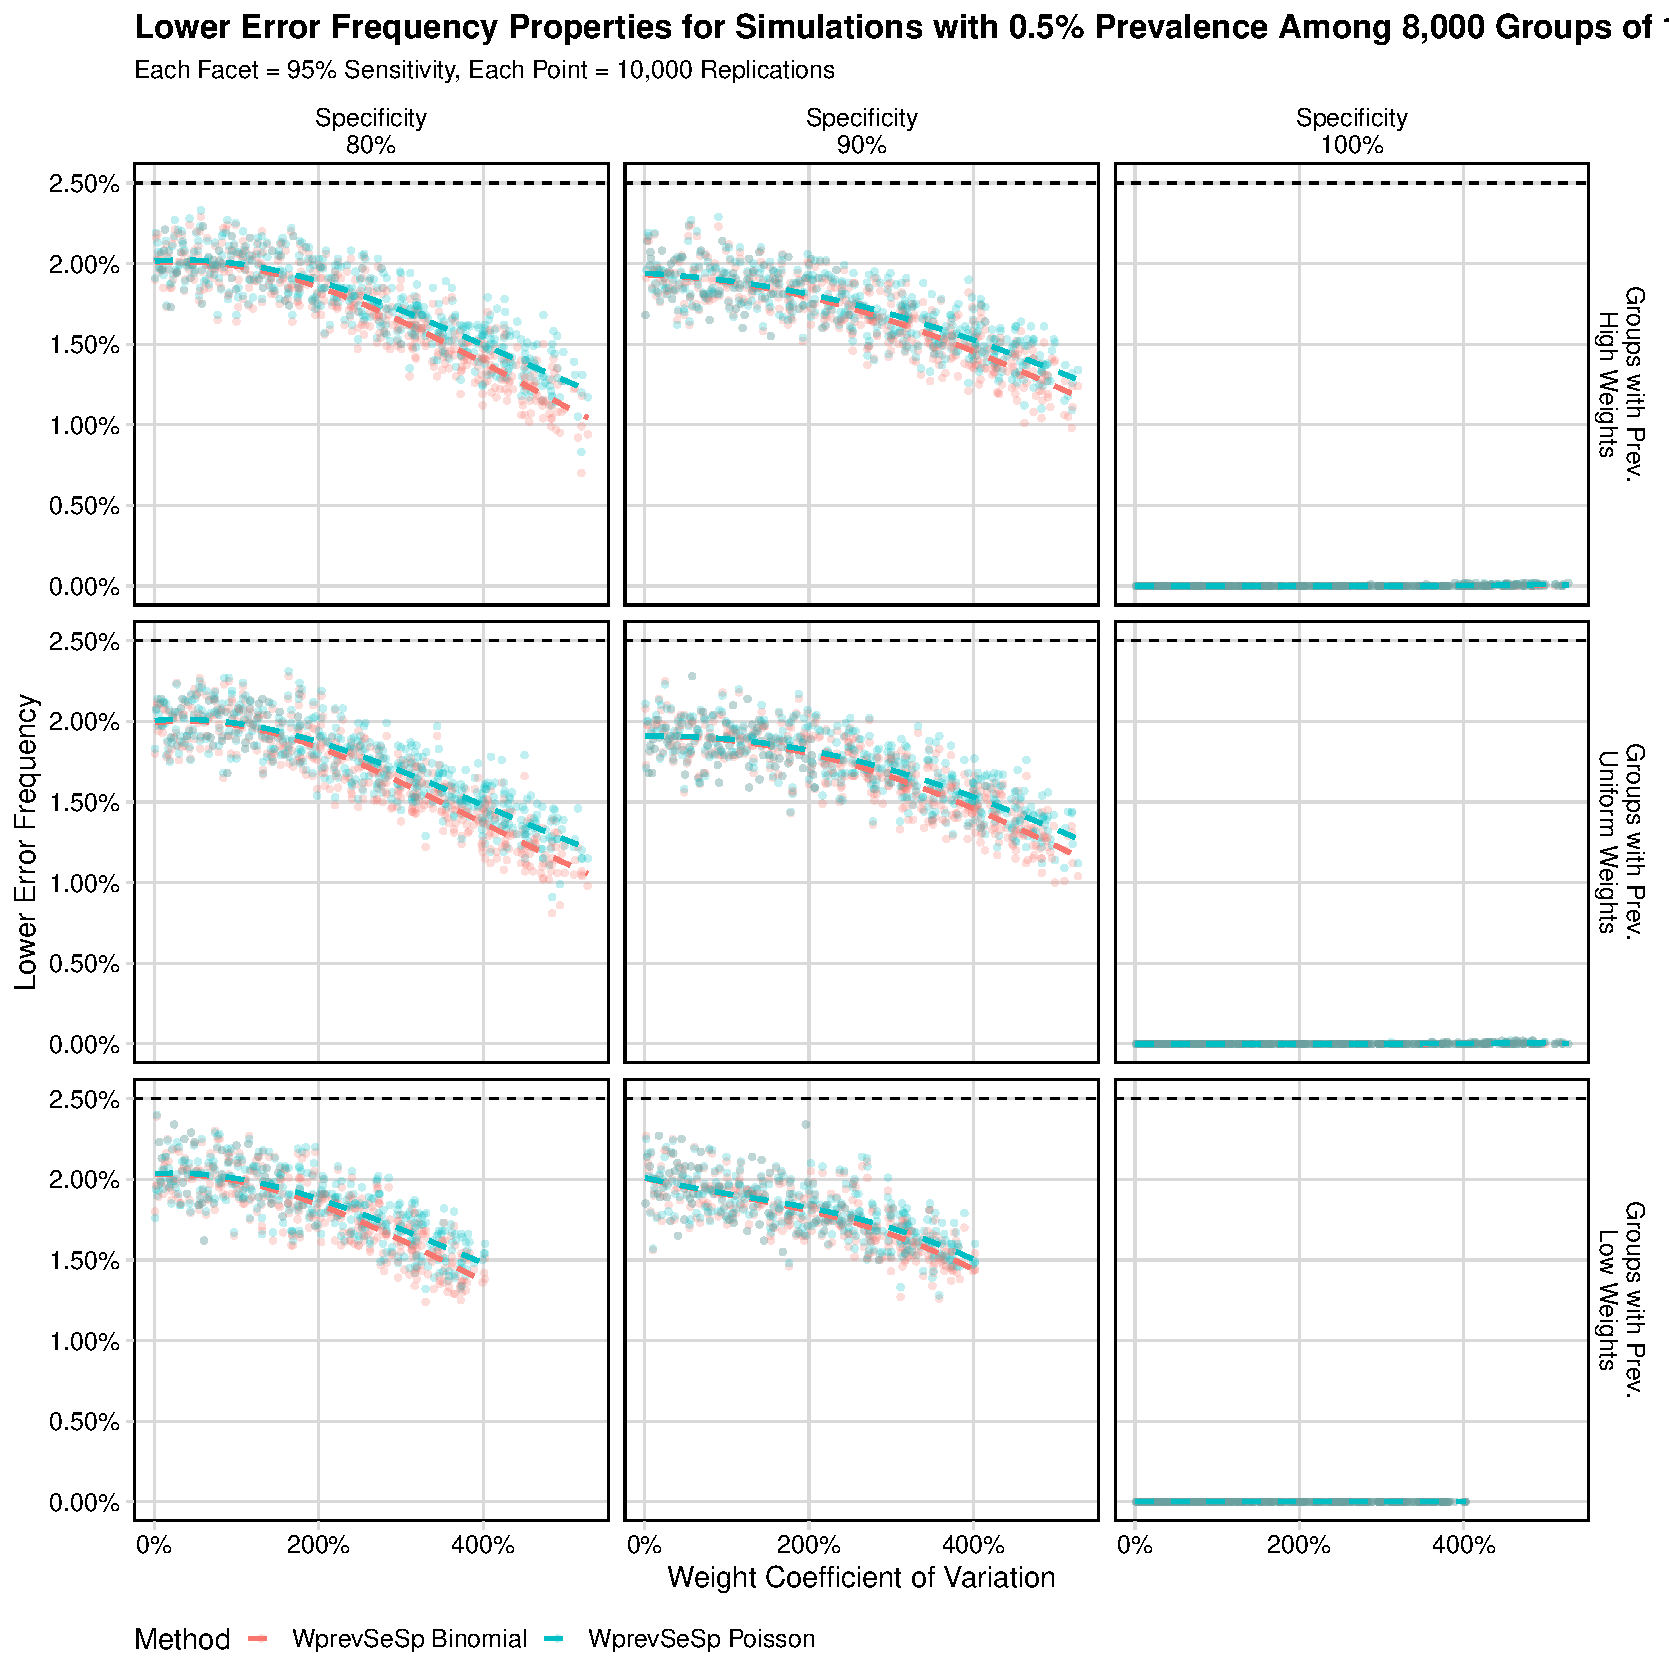
\includegraphics[width=0.8\textwidth]{figures/imperfect_lower_error_frequency_8000_groups_0_005_prev.pdf}
\caption{Lower error properties for the two melded confidence interval procedures, WprevSeSp Binomial and WprevSeSp Poisson, and one method, wspoissonTest, which does not account for the imperfect assay.
Each point represents 10,000 simulations of datasets from a population with 5\% Prevalence where 8000 individuals are sampled.
Each datasets also includes simulated results of tests to evaluate the sensitivity and specificity of the assay performed on 60 and 300 individuals, respectively.
The horizontal dashed line indicates the nominal lower error rate, 2.5\%.
Colored dashed lines are estimates from a logistic regression model using cubic splines.}
\label{fig:imperfect_lower_error_frequency_8000_groups_0_005_prev}
\end{figure}

\begin{figure}
\centering
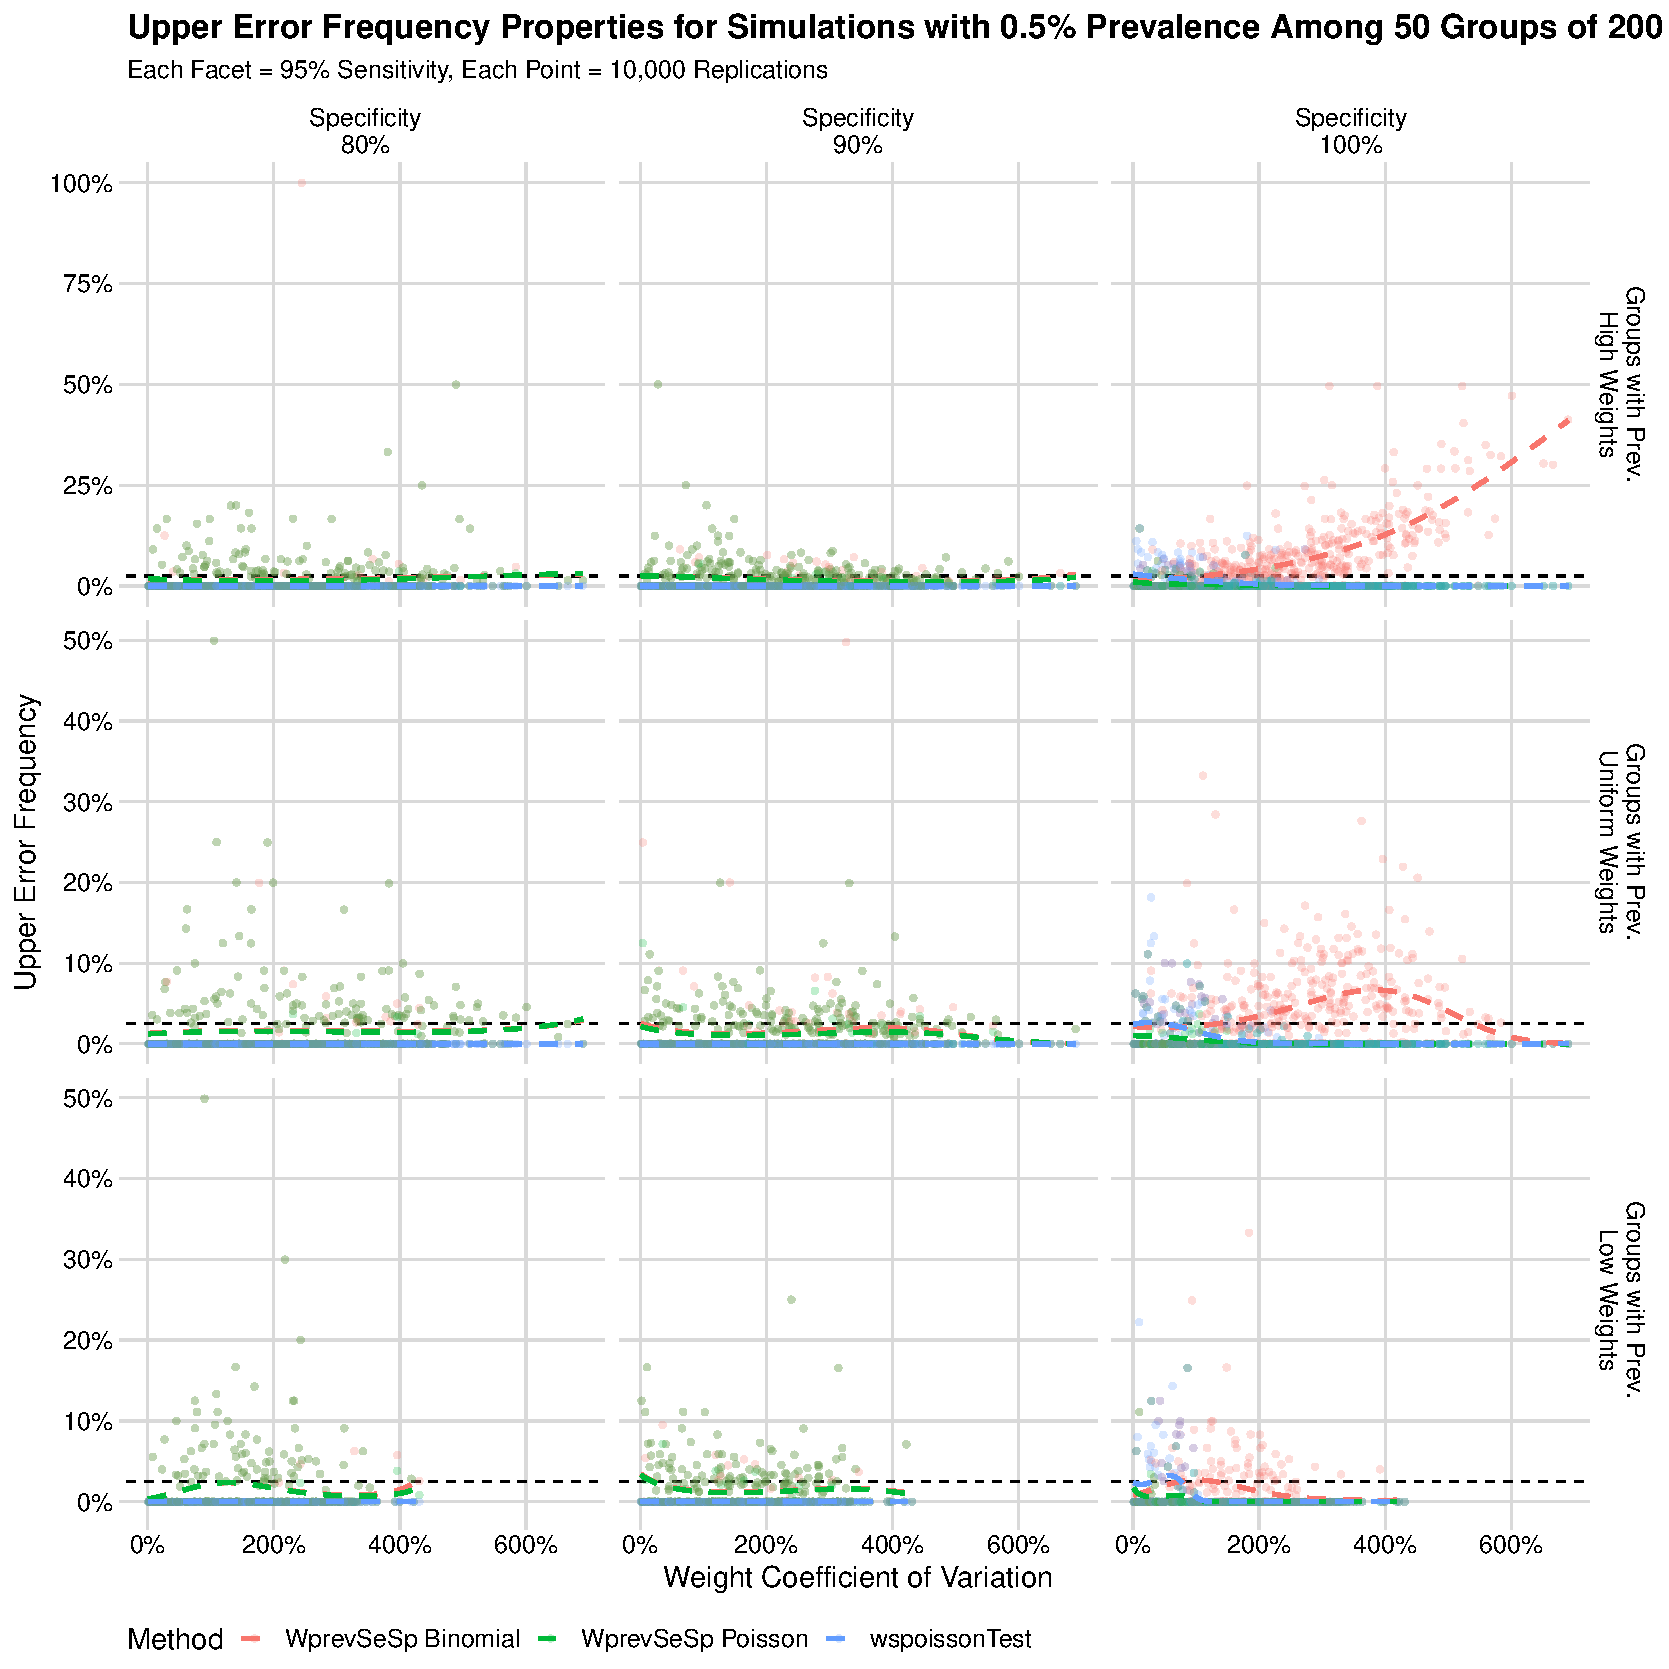
\includegraphics[width=0.8\textwidth]{figures/imperfect_upper_error_frequency_50_groups_0_005_prev.pdf}
\caption{Upper error properties for the two melded confidence interval procedures, WprevSeSp Binomial and WprevSeSp Poisson, and one method, wspoissonTest, which does not account for the imperfect assay.
Each point represents 10,000 simulations of datasets from a population with 0.5\% Prevalence where 50 groups of 200 people are sampled.
Each datasets also includes simulated results of tests to evaluate the sensitivity and specificity of the assay performed on 60 and 300 individuals, respectively.
The horizontal dashed line indicates the nominal upper error rate, 2.5\%.
Colored dashed lines are estimates from a logistic regression model using cubic splines.}
\label{fig:imperfect_upper_error_frequency_50_groups_0_005_prev}
\end{figure}

\begin{figure}
\centering
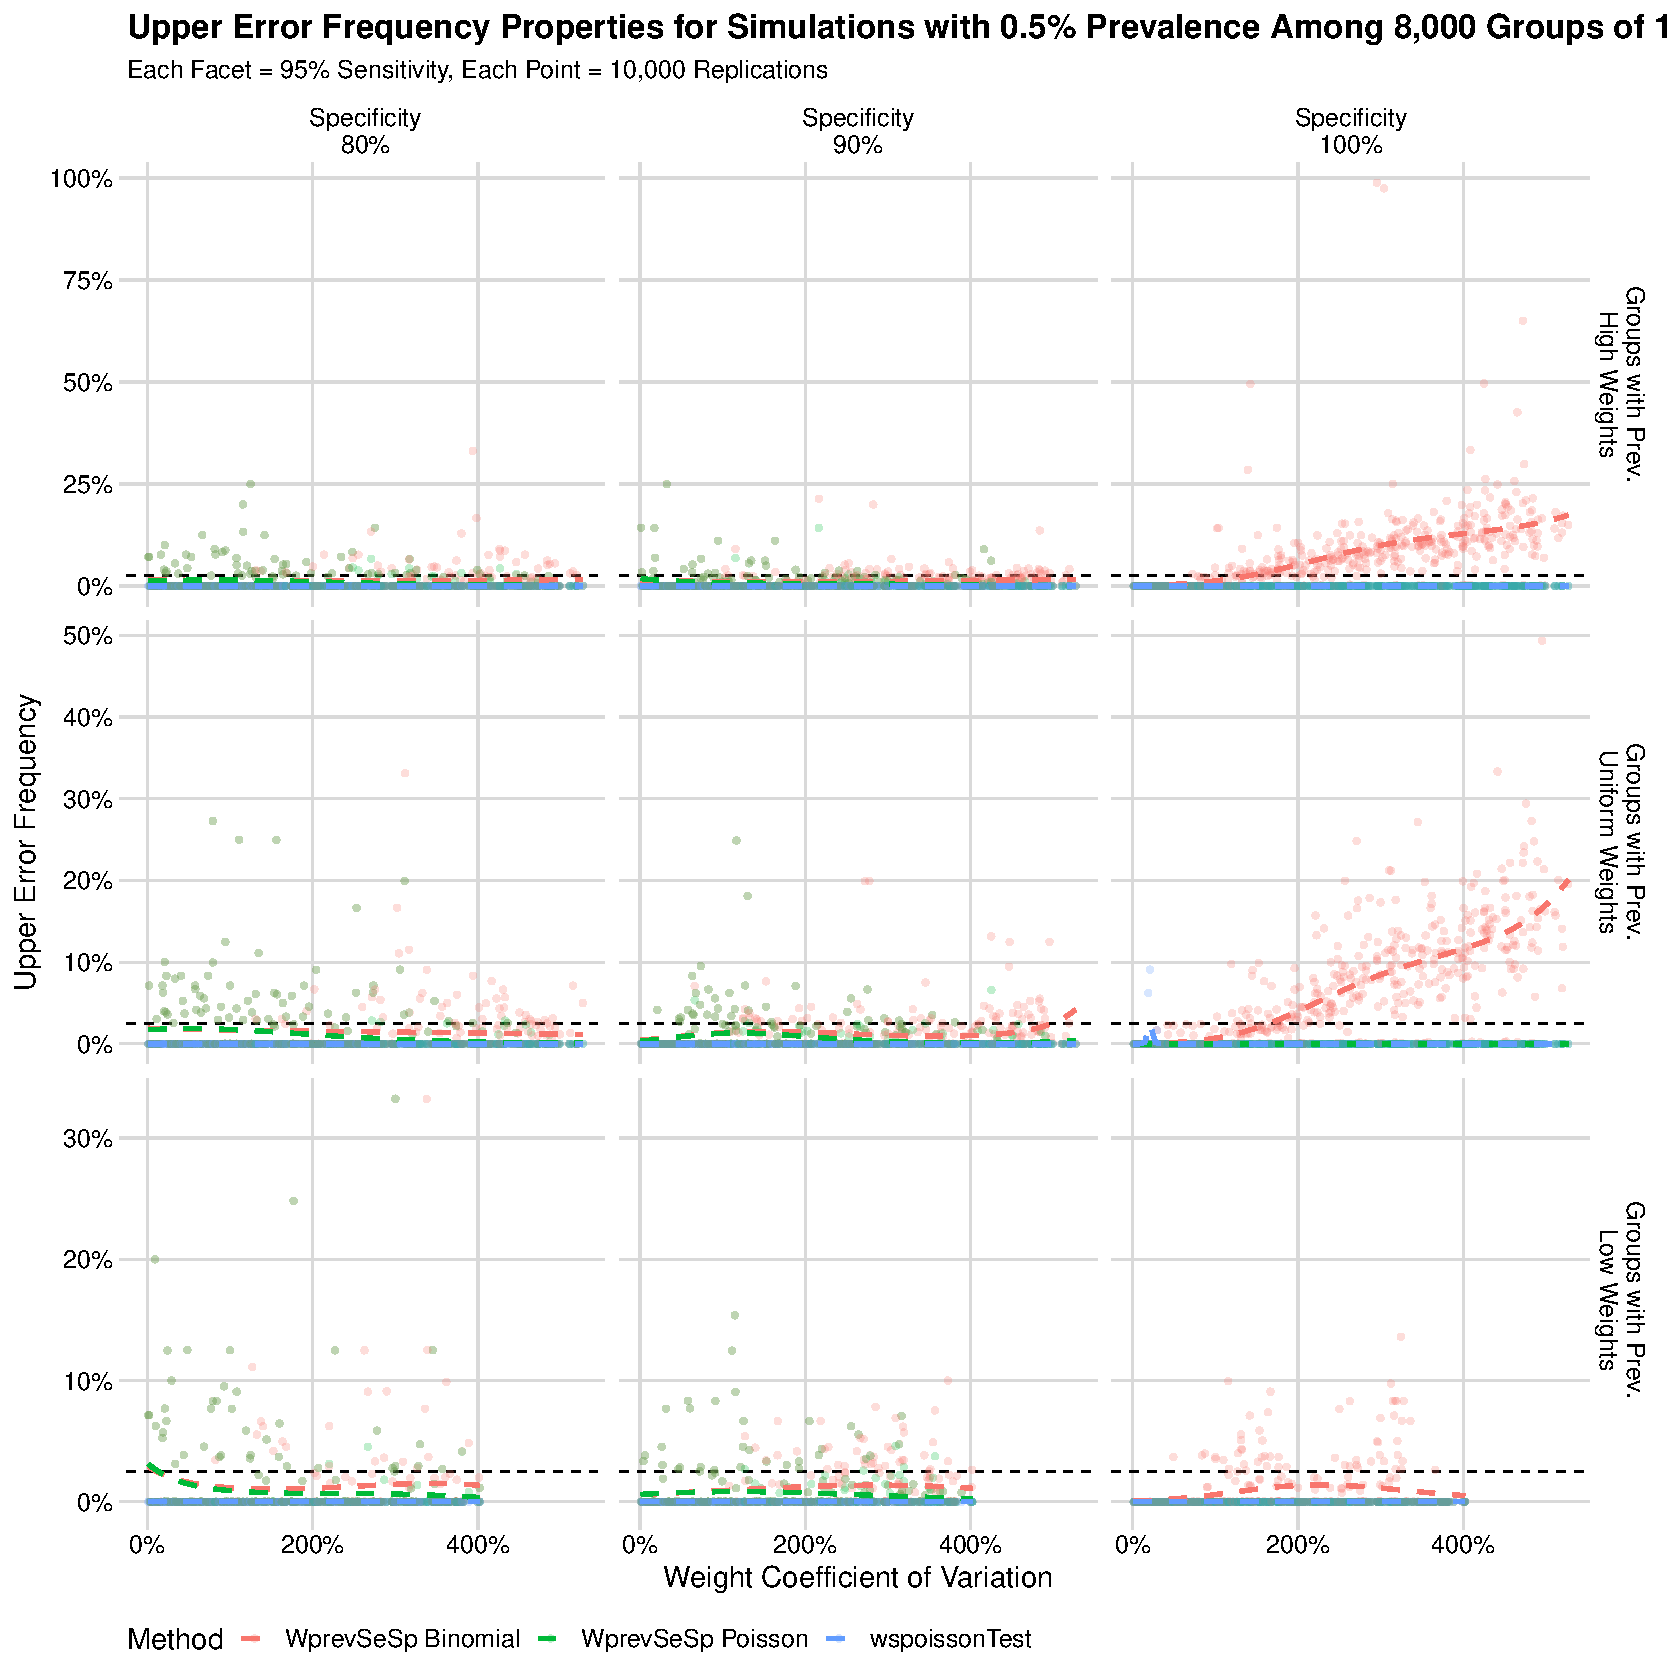
\includegraphics[width=0.8\textwidth]{figures/imperfect_upper_error_frequency_8000_groups_0_005_prev.pdf}
\caption{Upper error properties for the two melded confidence interval procedures, WprevSeSp Binomial and WprevSeSp Poisson, and one method, wspoissonTest, which does not account for the imperfect assay.
Each point represents 10,000 simulations of datasets from a population with 0.5\% Prevalence where 8000 individuals are sampled.
Each datasets also includes simulated results of tests to evaluate the sensitivity and specificity of the assay performed on 60 and 300 individuals, respectively.
The horizontal dashed line indicates the nominal upper error rate, 2.5\%.
Colored dashed lines are estimates from a logistic regression model using cubic splines.}
\label{fig:imperfect_upper_error_frequency_8000_groups_0_005_prev}
\end{figure}

\begin{figure}
\centering
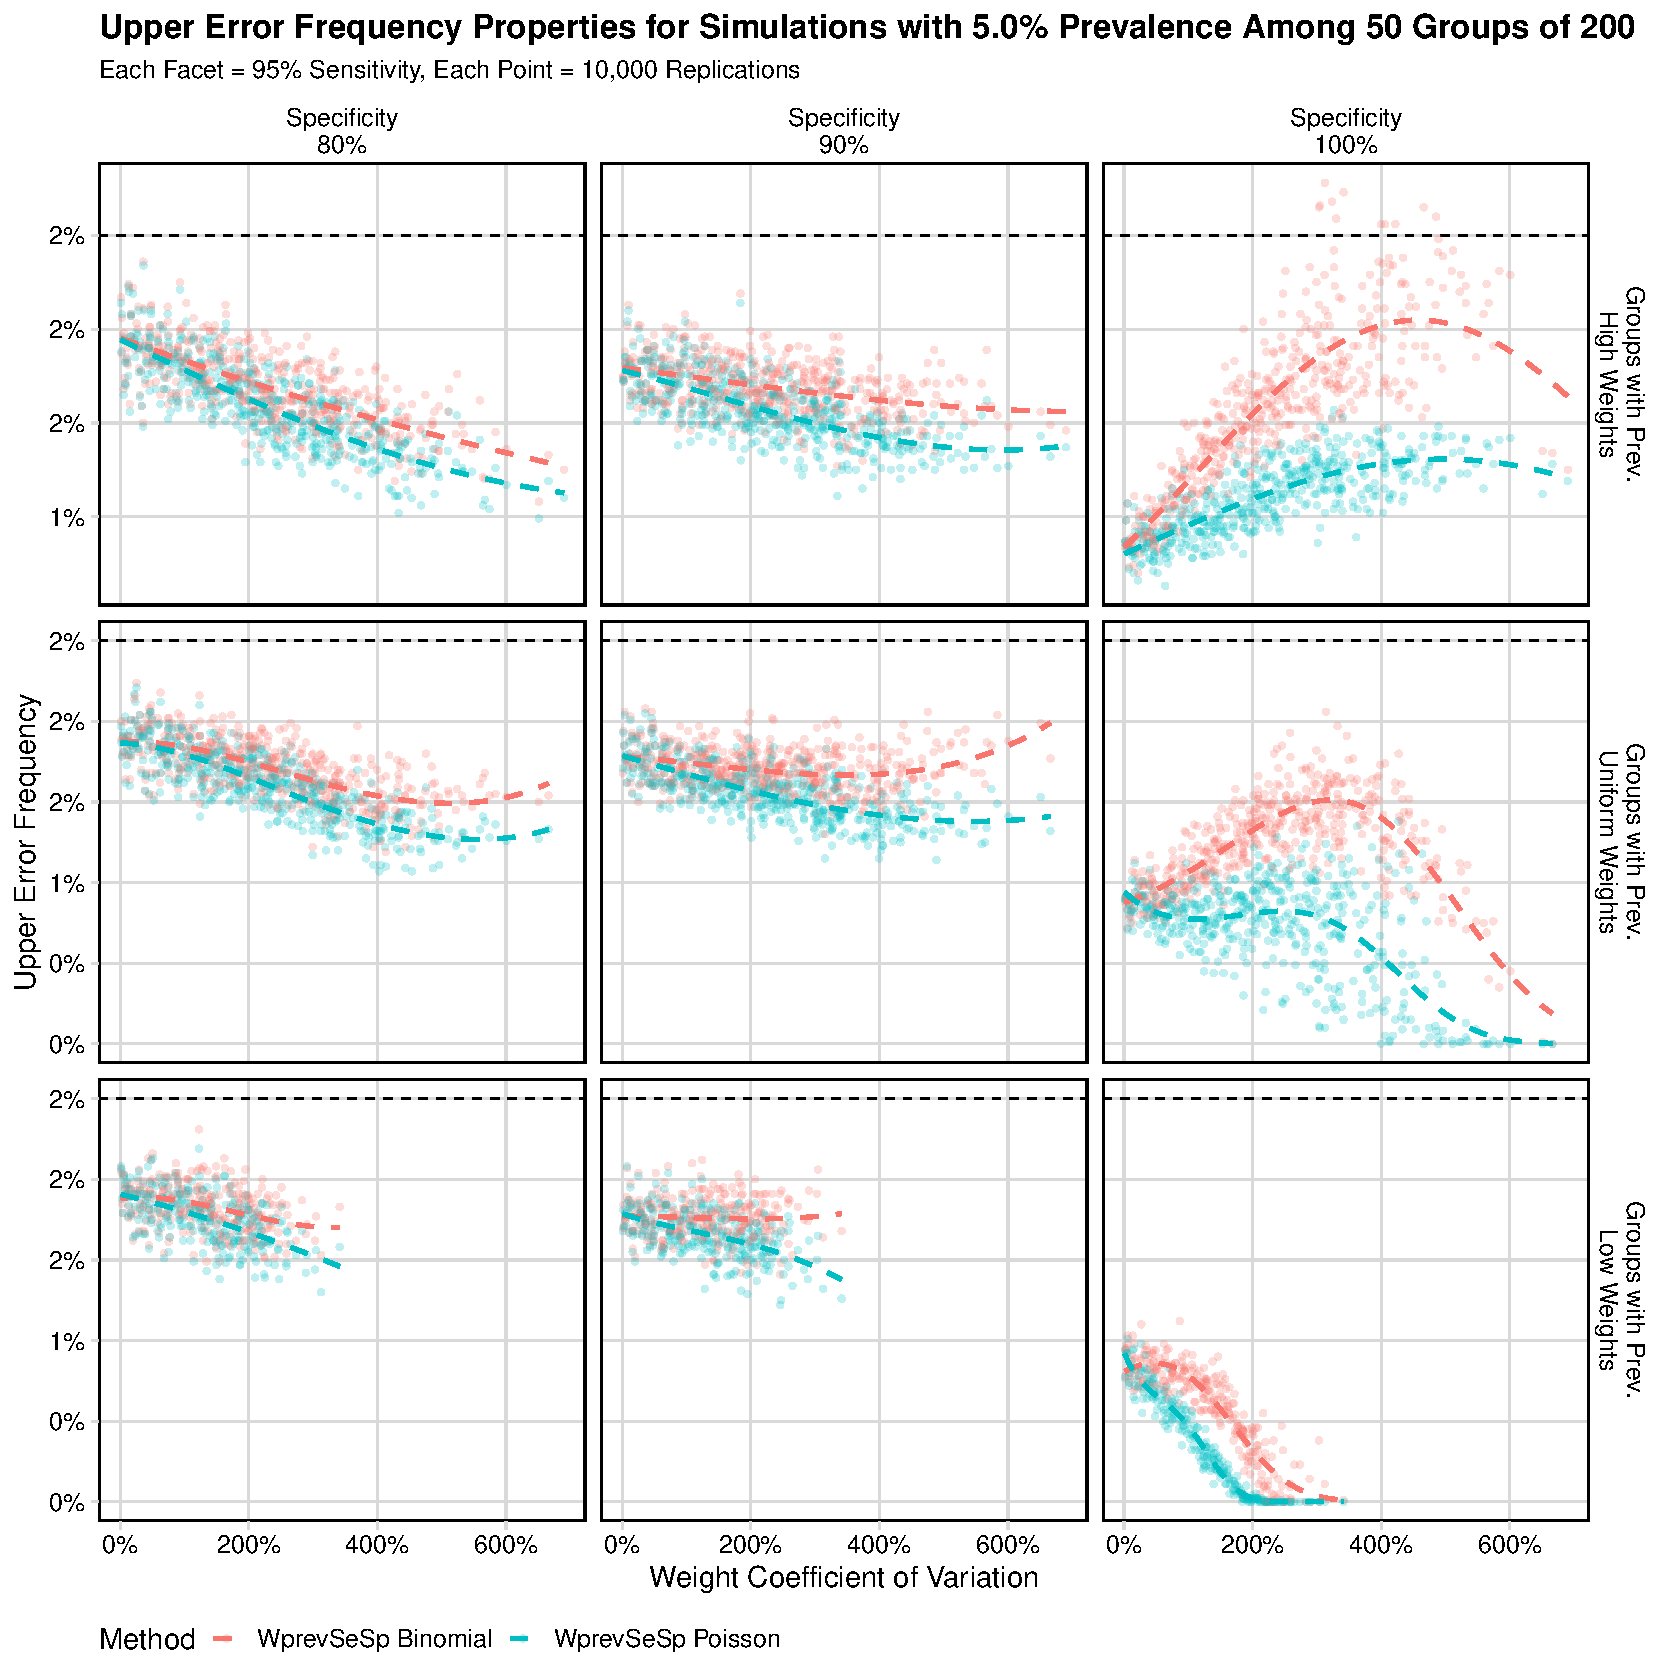
\includegraphics[width=0.8\textwidth]{figures/imperfect_upper_error_frequency_50_groups_0_05_prev.pdf}
\caption{Upper error properties for the two melded confidence interval procedures, WprevSeSp Binomial and WprevSeSp Poisson, and one method, wspoissonTest, which does not account for the imperfect assay.
Each point represents 10,000 simulations of datasets from a population with 5\% Prevalence where 50 groups of 200 people are sampled.
Each datasets also includes simulated results of tests to evaluate the sensitivity and specificity of the assay performed on 60 and 300 individuals, respectively.
The horizontal dashed line indicates the nominal upper error rate, 2.5\%.
Colored dashed lines are estimates from a logistic regression model using cubic splines.}
\label{fig:imperfect_upper_error_frequency_50_groups_0_05_prev}
\end{figure}

\begin{figure}
\centering
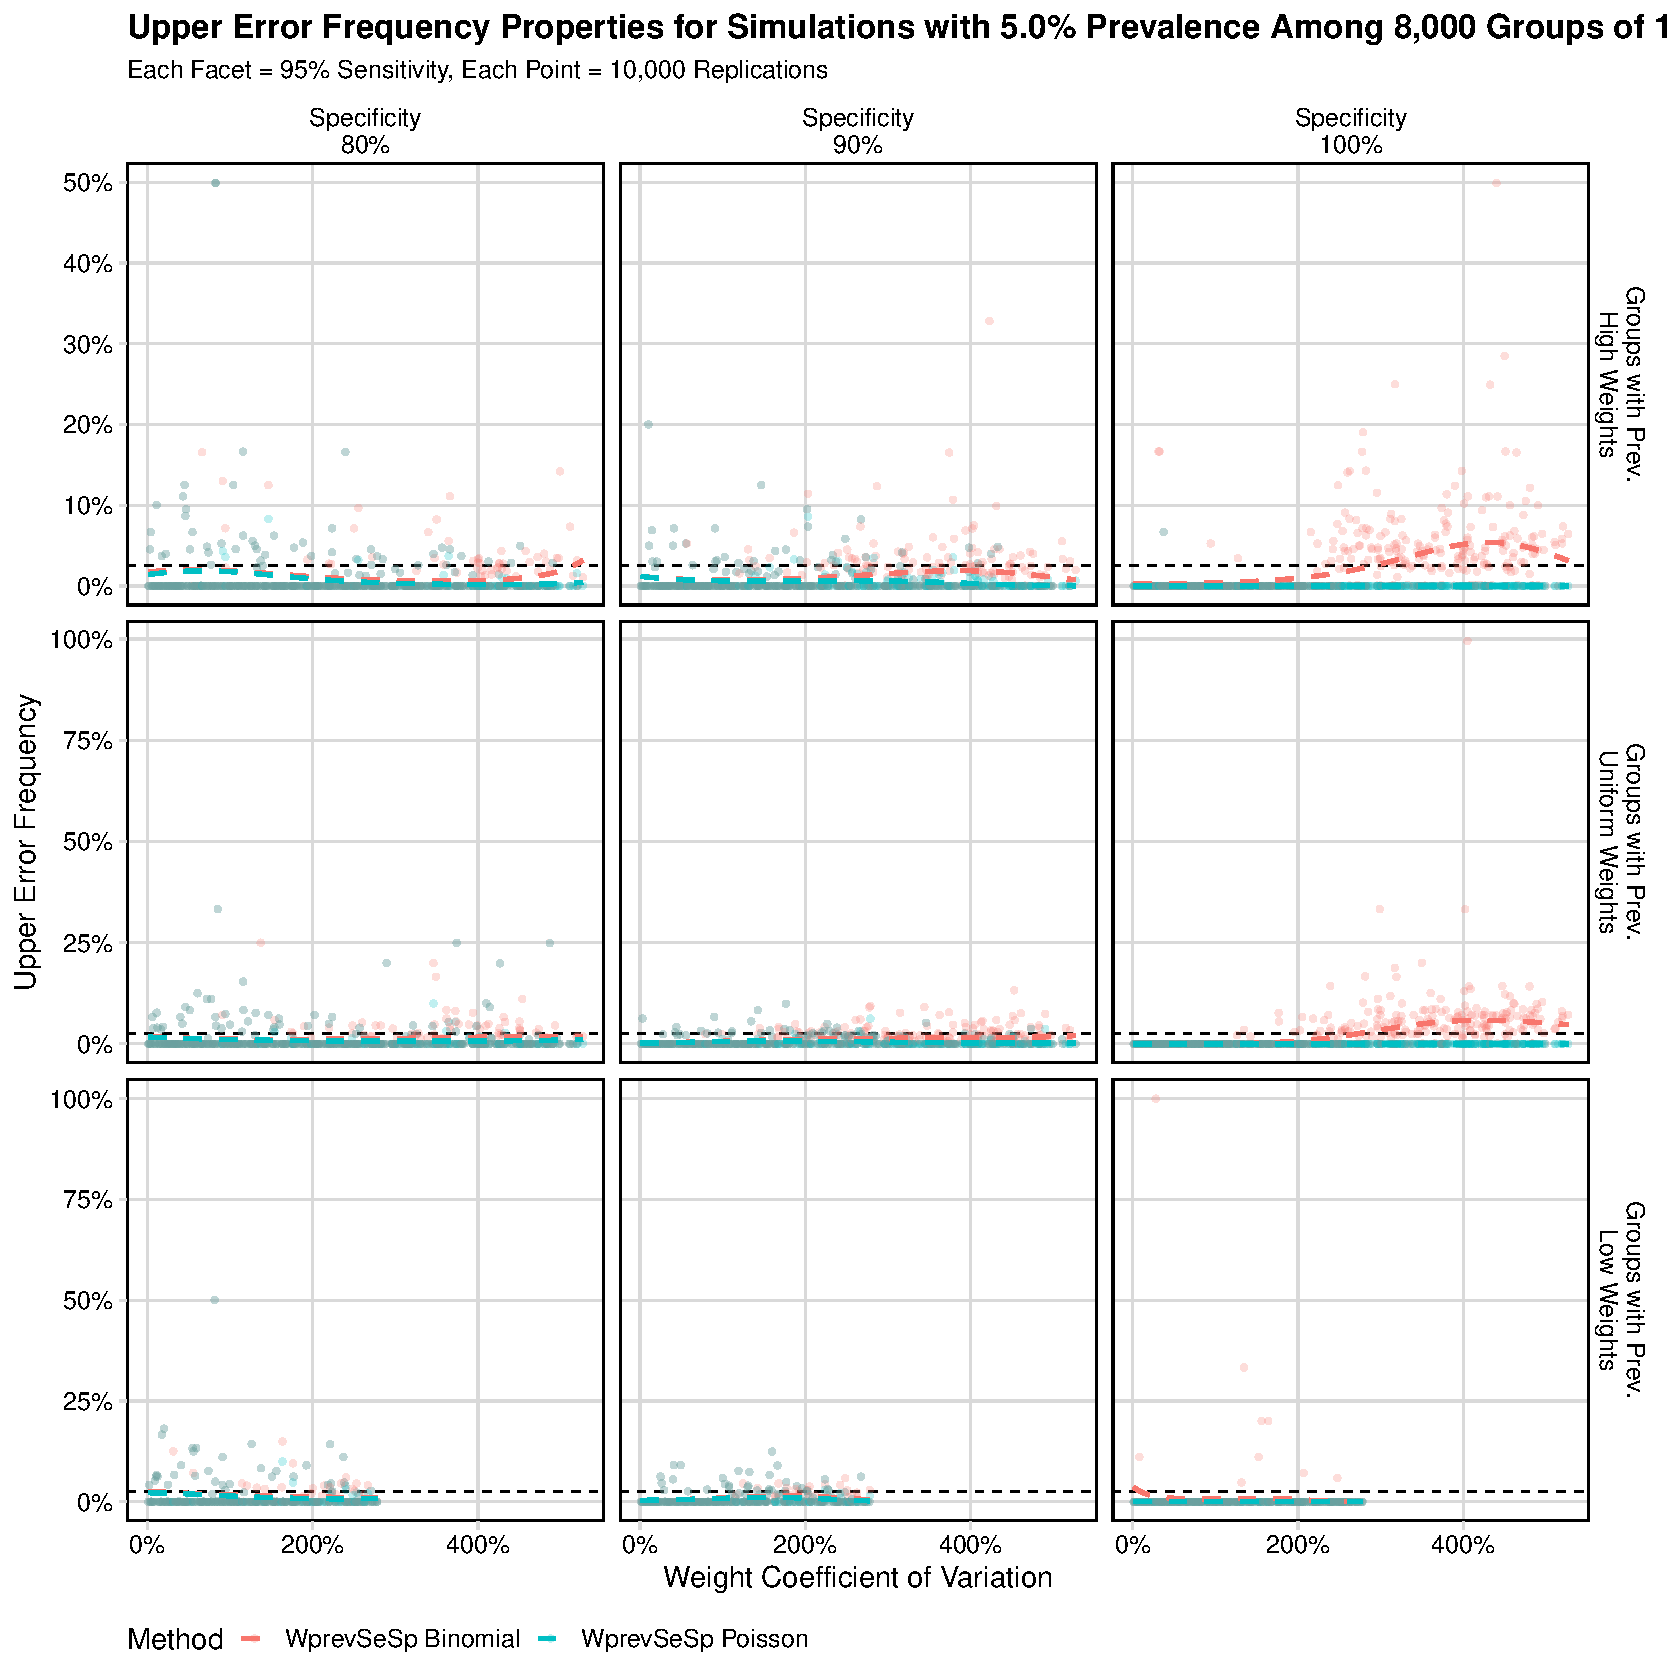
\includegraphics[width=0.8\textwidth]{figures/imperfect_upper_error_frequency_8000_groups_0_05_prev.pdf}
\caption{Upper error properties for the two melded confidence interval procedures, WprevSeSp Binomial and WprevSeSp Poisson, and one method, wspoissonTest, which does not account for the imperfect assay.
Each point represents 10,000 simulations of datasets from a population with 5\% Prevalence where 8000 individuals are sampled.
Each datasets also includes simulated results of tests to evaluate the sensitivity and specificity of the assay performed on 60 and 300 individuals, respectively.
The horizontal dashed line indicates the nominal upper error rate, 2.5\%.
Colored dashed lines are estimates from a logistic regression model using cubic splines.}
\label{fig:imperfect_upper_error_frequency_8000_groups_0_05_prev}
\end{figure}



\end{document}